% !TEX program = xelatex
% weekly review deck 2026-11-02 to 11-08, self-contained
\documentclass[aspectratio=169,10pt,fontset=none]{ctexbeamer}
% ===== 共享导言区：分片 wrapper 与最终成品共用 =====
% 最终 Attachments/daily-exercise-weekly-review-2026-11-02-to-08.tex 自包含本文件内容。
\usepackage{fontspec}
\setCJKmainfont{Microsoft YaHei}
\setCJKsansfont{Microsoft YaHei}

\usepackage{amsmath,amssymb}
\usepackage{mathtools}
\usepackage{booktabs}
\usepackage{array}
\usepackage{colortbl}
\usepackage{graphicx}
\graphicspath{{./}{Attachments/}{../Attachments/}{../../Attachments/}{../../../Attachments/}}
\usepackage{tikz}
\usetikzlibrary{arrows.meta,positioning,calc}

% ---------- 配色（沿用库内讲义配色） ----------
\definecolor{ink}{HTML}{1F3864}
\definecolor{accent}{HTML}{C00000}
\definecolor{gold}{HTML}{BF8F00}
\definecolor{greenink}{HTML}{2E6B2E}
\definecolor{paper}{HTML}{F5F7FA}

\usetheme{default}
\usecolortheme[named=ink]{structure}
\setbeamertemplate{navigation symbols}{}
\setbeamertemplate{itemize items}[circle]
\setbeamercolor{structure}{fg=ink}
\setbeamercolor{frametitle}{fg=ink}
\setbeamercolor{block title}{bg=ink!12,fg=ink}
\setbeamercolor{block body}{bg=ink!4,fg=black}
\setbeamercolor{block title alerted}{bg=accent!12,fg=accent}
\setbeamercolor{block body alerted}{bg=accent!4,fg=black}
\setbeamercolor{block title example}{bg=greenink!14,fg=greenink}
\setbeamercolor{block body example}{bg=greenink!5,fg=black}
\setbeamerfont{frametitle}{size=\large,series=\bfseries}
\setbeamerfont{footline}{size=\scriptsize}
\setbeamertemplate{frametitle}{\vskip3pt\insertframetitle\par\vskip1.5pt%
  \textcolor{accent}{\rule{\textwidth}{0.7pt}}\vskip-3pt}
\setbeamertemplate{footline}{%
  \hbox to \paperwidth{\hspace{8pt}%
    \textcolor{ink!55}{本周 Daily Exercise 回顾\ \ ·\ \ 11-02 -- 11-08\ \ ·\ \ 42 题详解版}\hfill
    \textcolor{ink!55}{\insertframenumber\,/\,\inserttotalframenumber}\hspace{9pt}}\vskip5pt}
\setbeamersize{text margin left=0.75cm,text margin right=0.75cm}
\setlength{\parindent}{0pt}
\setlength{\parskip}{2pt}
\AtBeginDocument{%
  \setlength{\abovedisplayskip}{3pt}\setlength{\belowdisplayskip}{3pt}%
  \setlength{\abovedisplayshortskip}{2pt}\setlength{\belowdisplayshortskip}{2pt}}

% 题号标记
\newcommand{\ex}[1]{\textcolor{accent}{\footnotesize\bfseries #1}}
\newcommand{\key}[1]{\textcolor{ink}{\bfseries #1}}
\newcommand{\starpt}{\textcolor{accent}{\bfseries$\ast$}}

\hypersetup{pdftitle={本周 Daily Exercise 回顾（2026-11-02 至 11-08，42 题详解版）},
  pdfsubject={Artin Algebra 2e, Ch. 6 Sections 3--12 and M.1, Ch. 7 Sections 10--11 and M.1--M.9, Ch. 8 Section 1: 42 exercises weekly review},
  pdfauthor={exercise\_abstract}}
\title{本周 Daily Exercise 回顾（2026-11-02 至 11-08，42 题详解版）}
\author{exercise\_abstract}

\begin{document}
% ============================================================ 1 标题页
\begin{frame}[plain]
\pdfbookmark[1]{封面}{bm:cover}
  \begin{tikzpicture}[remember picture,overlay]
    \fill[ink] (current page.north west) rectangle ([yshift=-4.75cm]current page.north east);
    \node[anchor=north west,text=white,font=\fontsize{25}{29}\selectfont\bfseries]
      at ([xshift=1.0cm,yshift=-0.92cm]current page.north west) {本周 Daily Exercise 回顾};
    \node[anchor=north west,text=white!90]
      at ([xshift=1.02cm,yshift=-2.08cm]current page.north west)
      {\large 覆盖 2026-11-02 -- 11-08（7 份清单，42 题）\quad·\quad 逐题详解版};
    \node[anchor=north west,text=white!75]
      at ([xshift=1.02cm,yshift=-2.86cm]current page.north west)
      {\small Artin \textit{Algebra} 2e：Ch.~6 \S3--\S12 + M.1，Ch.~7 \S10--\S11 + M.1--M.9，Ch.~8 \S1\quad·\quad 群论 39 + 线代 3\quad·\quad 难度 5/11/26};
    \node[anchor=north east,text=white!60,font=\small]
      at ([xshift=-1.0cm,yshift=-0.92cm]current page.north east) {exercise\_abstract};
    \node[anchor=west,text=white!55,font=\tiny]
      at ([xshift=1.02cm,yshift=-4.45cm]current page.north west)
      {数据来源：\texttt{10 - Daily Exercise Lists} 的 7 份清单；题面与来源取自 42 篇习题笔记并经原书 PDF 核对；数学结论经独立复核与程序验算；快照 2026-11-08 16:25};
  \end{tikzpicture}
  \vspace*{4.9cm}
  \begin{columns}[T,onlytextwidth]
    \begin{column}{0.50\textwidth}
      \begin{block}{两条主线（本周清单的两区）}
        \scriptsize
        \begin{itemize}\setlength{\itemsep}{1pt}
          \item \key{Random Review（21 题，Artin Ch.~6）}\\
                平面等距的复坐标与复合、离散群与饰带、稳定化子与群作用、多面体/立方体/二十面体、壁纸点群与晶体学、格与矩阵、$D_{10}$ 的陪集与商群
          \item \key{Systematic Progress（21 题，Ch.~7 \S10--\S11 + M.1--M.9 + Ch.~8 \S1）}\\
                换位子群与正规闭包、表现与 Todd--Coxeter、三角形群、双陪集、同构定理、左右陪集基数、奇阶共轭、对称/反对称分解
        \end{itemize}
      \end{block}
    \end{column}
    \begin{column}{0.47\textwidth}
      \begin{block}{这一版的用法与边界}
        \scriptsize
        \begin{itemize}\setlength{\itemsep}{1pt}
          \item 每题：完整题面 → 一句思路 → \textbf{显示中间式的推导} → 具体验算/反例
          \item 7 份清单全部存在（11-02 至 11-08 逐日生成），共 42 题，互不重复
          \item 这是\textbf{快照}：11-08 题单于 16:21 读取；题单若之后追加，以库内文件为准
          \item 第 \pageref{sec:answers} 页起是 42 题速查表、方法卡、易错点与自测
        \end{itemize}
      \end{block}
    \end{column}
  \end{columns}
\end{frame}

% ============================================================ 2 本周概览
\begin{frame}[t]{一、本周概览：7 份题单、42 题、两个独立队列}
  \label{sec:overview}
\pdfbookmark[1]{一、本周概览}{bm:sec-overview}
  \centering
  \scriptsize
  \setlength{\tabcolsep}{3pt}
  \renewcommand{\arraystretch}{1.14}
  \begin{tabular}{@{}l l l@{}}
    \toprule
    日期 & Random Review（3 题） & Systematic Progress（3 题）\\
    \midrule
    11-02（一） & G183，G111，G185 & G247，LA308，G248\\
    11-03（二） & G158，G114，G177 & G249，G250，G251\\
    11-04（三） & G107，G165，G160 & G252，G253，G254\\
    11-05（四） & LA193，G172，G187 & G255，G256，G257\\
    11-06（五） & G17，G148，G113 & G258，G259，G260\\
    \rowcolor{ink!7} 11-07（六） & G162，G178，G19 & G261，G262，G263\\
    \rowcolor{ink!7} 11-08（日） & G110，G169，G25 & G264，G265，LA201\\
    \midrule
    合计 & \textbf{21} 题（Ch.~6） & \textbf{21} 题（Ch.~7--8）\\
    \bottomrule
  \end{tabular}
  \vspace{0.35em}
  \raggedright
  \begin{columns}[T,onlytextwidth]
    \begin{column}{0.49\textwidth}
      \begin{exampleblock}{\footnotesize 数据观察}
        \scriptsize
        \begin{itemize}\setlength{\itemsep}{1pt}
          \item \textbf{7 天题单齐全}：11-02 至 11-08 每天都有 Random 与 Systematic 两区各 3 题；本周无缺日。
          \item \textbf{42 题互不重复}，随机区覆盖 Ch.~6 \S3--\S12 与 M.1，系统区从 \S10 接上周的 Ex.~10.7，经 \S11 到 M.1--M.9，再进入 Ch.~8 \S1。
          \item Random 与 Systematic 是两条独立队列；随机区抽题不推进系统进度，本讲义也不改动任何学习状态。
        \end{itemize}
      \end{exampleblock}
    \end{column}
    \begin{column}{0.49\textwidth}
      \begin{block}{\footnotesize 难度、来源与快照}
        \scriptsize
        入门 5 · 中等 11 · 高级 26。\\
        Artin 2e：Ch.~6 印刷 pp.~188--193 / PDF pp.~200--205（G148 引 Fig.~6.6.2，印刷 p.~174 / PDF p.~186）；Ch.~7 印刷 pp.~226--227 / PDF pp.~238--239；Ch.~8 印刷 p.~254 / PDF p.~266；另含 Lang I.10（印刷 p.~75 / PDF p.~90）。\\[1pt]
        \starpt 快照：2026-11-08 16:25（11-08 题单读取时间）；7 份清单的哈希前缀已记入 CHANGELOG，题单之后若追加，以库内文件为准。
      \end{block}
    \end{column}
  \end{columns}
\end{frame}

% ============================================================ 3 议程
\begin{frame}[t]{二、怎么用：150 分钟议程与三种用法}
  \label{sec:agenda}
\pdfbookmark[1]{二、怎么用}{bm:sec-agenda}
  \begin{columns}[T,onlytextwidth]
    \begin{column}{0.54\textwidth}
      \centering
      \scriptsize
      \setlength{\tabcolsep}{3pt}
      \renewcommand{\arraystretch}{1.2}
      \begin{tabular}{@{}l l r@{}}
        \toprule
        时间 & 内容 & 页\\
        \midrule
        15 分钟 & 两条工具线 & \pageref{sec:framework1}\\
        55 分钟 & 随机 21 题 & \pageref{sec:random}\\
        60 分钟 & 系统 21 题 & \pageref{sec:sys}\\
        20 分钟 & 速查与自测 & \pageref{sec:answers}\\
        \bottomrule
      \end{tabular}
    \end{column}
    \begin{column}{0.43\textwidth}
      \begin{block}{\footnotesize 三种用法}
        \scriptsize
        \begin{itemize}\setlength{\itemsep}{1pt}
          \item \textbf{通读}：每题“题面 → 思路 → 详解 → 验算”完整走一遍；
          \item \textbf{讲题}：先让学生说该算哪个量，再翻到详解页对照；
          \item \textbf{复习}：只看第 \pageref{sec:answers} 页起的速查表与方法卡，忘了再回跳。
        \end{itemize}
      \end{block}
      \begin{alertblock}{\footnotesize 时间不够时的取舍}
        \scriptsize
        42 题一次讲完偏紧，建议分两次：先 Random（第 \pageref{sec:random} 页起），再 Systematic（第 \pageref{sec:sys} 页起）。若只有 60 分钟，优先分配给出题面与推导最长的题目（G250、G251、G256、G148、G187），其余快速过结论后回到速查表。
      \end{alertblock}
    \end{column}
  \end{columns}
  \vspace{0.2em}
  {\scriptsize\color{ink!70} 页脚给出当前页/总页数；所有页码引用由 \LaTeX{} 标签自动生成，增删页面后重编译即可同步。}
\end{frame}

% ============================================================ 4 框架 1/2
\begin{frame}[t]{三、框架 1/2：Random Review 的工具箱（Artin Ch.~6 \S3--\S12 + M.1）}
  \label{sec:framework1}
\pdfbookmark[1]{三、框架 1/2：Random Review 工具箱}{bm:sec-framework1}
  \begin{columns}[T,onlytextwidth]
    \begin{column}{0.49\textwidth}
      \begin{block}{\footnotesize 平面等距、复坐标与复合}
        \scriptsize
        $M=\{\text{平移}\}\rtimes O(2)$；以 $z=x+iy$ 记点、$a=a_1+ia_2$ 记平移向量，则
        \[ t_a(z)=z+a,\quad \rho_\theta(z)=e^{i\theta}z,\quad r(z)=\overline z, \]
        保向等距为 $m(z)=a+e^{i\theta}z$，反向为 $a+e^{i\theta}\overline z$（G17、G19）。\\
        关于直线 $\ell$ 的稳定化子由方向约束 $A\ell_0=\ell_0$ 与平移约束 $u\in\ell$ 解出（G111、G113）；旋转的复合给出平移（G114）。
      \end{block}
      \begin{block}{\footnotesize 稳定化子、轨道与作用}
        \scriptsize
        轨道–稳定化子：$|Gs|=[G:G_s]$；传递作用 $\cong$ 陪集作用（G162）。\\
        忠实性看核 $\bigcap_s G_s$；五点作用分成 $3+2$ 两个轨道时 $G\hookrightarrow S_3\times S_2$（G177）。\\
        “平移集均匀覆盖”用双计数得到 $N=|U|\,|G_s|$（G172）；正方形顶点、立方体、二十面体的稳定化子逐点算（G162、G165、G183、G185）。
      \end{block}
    \end{column}
    \begin{column}{0.49\textwidth}
      \begin{block}{\footnotesize 多面体、立方体与二十面体}
        \scriptsize
        旋转群：$T\cong A_4$（12），$O\cong S_4$（24），$I\cong A_5$（60）；允许反射时阶翻倍（G158）。\\
        立方体旋转群 $O$ 在四个体对角线上传递，稳定化子阶 $24/4=6$，同构于 $D_3$（G183）；二十面体群含 5 阶旋转，故有 10 阶子群（G185）；$S_4$ 中 12 阶子群唯一为 $A_4$（G160）。
      \end{block}
      \begin{block}{\footnotesize 壁纸点群、晶体学与格}
        \scriptsize
        平面点群只能是 $C_n$ 或 $D_n$，$n\in\{1,2,3,4,6\}$；17 个壁纸型按旋转阶与镜/滑移分类（G148）。\\
        无不动点的二维晶体群由两个平移、或一平移一滑移生成（G187）；阶梯饰带的点群 $D_2$、平移指数 4（G110）；棒球接缝群 $D_2$（G169）。\\
        格基变换矩阵 $P\in GL_2(\mathbb Z)$ 即 $\det P=\pm1$（LA193）；$D_{10}\cong D_5\times C_2$ 的陪集分解（G25）。
      \end{block}
    \end{column}
  \end{columns}
\end{frame}

% ============================================================ 5 框架 2/2
\begin{frame}[t]{三、框架 2/2：Systematic Progress 的工具箱（Artin Ch.~7 \S10--\S11 + M + Ch.~8 \S1）}
  \label{sec:framework2}
\pdfbookmark[1]{三、框架 2/2：Systematic Progress 工具箱}{bm:sec-framework2}
  \begin{columns}[T,onlytextwidth]
    \begin{column}{0.49\textwidth}
      \begin{block}{\footnotesize 换位子群、正规闭包与自由群}
        \scriptsize
        $[G,G]=\langle g h g^{-1}h^{-1}\rangle$ 是最小的“商群交换”的正规子群；$G^{ab}=G/[G,G]$。\\
        $[SO_2,SO_2]=1$，$[O_2,O_2]=SO_2$，$[M,M]=M^+$，$[S_n,S_n]=A_n$，$[SO_3,SO_3]=SO_3$（G247）。\\
        单位上三角 Heisenberg 群：$Z(G)=[G,G]=\{\text{中心矩阵}\}$，元素阶 $1$ 或 $p$（LA308）。\\
        自由群 $F(x,y)$ 中一个换位子的正规闭包等于 $[F,F]$（G248）；两个对合生成的群由 $x^2=y^2=1$ 与 $xy$ 的阶刻画（G257）。
      \end{block}
      \begin{block}{\footnotesize 表现、Todd--Coxeter 与三角形群}
        \scriptsize
        表现 $\langle X\mid R\rangle$ 的群论后果直接用关系代入：$x^4=y^3=1,\ x^2=yxy\Rightarrow G=1$（G253）。\\
        Todd--Coxeter 陪集表给出指数与阶：$(7.8.2)$ 阶 12、$(7.7.8)$ 阶 21（G250），Ex.~11.3 十个表现逐个定阶（G251）；正规性等价于陪集表的“核”结构（G252）。\\
        三角形群 $G^{pqr}=\langle x,y,z:x^p=y^q=z^r=xyz=1\rangle$：$(2,2,n)\cong D_n$，$(2,3,4)\cong O$，$(2,3,5)\cong I$（G254--G256）。
      \end{block}
    \end{column}
    \begin{column}{0.49\textwidth}
      \begin{block}{\footnotesize 双陪集、同构定理与标准技巧}
        \scriptsize
        双陪集 $HgH$ 与 $G$ 在 $H\backslash G/H$、以及传递 $G$-集 $S$ 上 $S\times S$ 的轨道一一对应（G258、G259）。\\
        第二同构定理：$H/(H\cap N)\cong HN/N$；第三同构定理：$G/H\cong (G/N)/(H/N)$（G261、G262）。\\
        正规性不传递（G260 用 $V_4\triangleleft A_4$ 的反例）；奇阶群中 $x$ 与 $x^{-1}$ 不共轭（G265）；左右陪集基数对无限指数也用双射比较（G264）。
      \end{block}
      \begin{block}{\footnotesize 双线性形式}
        \scriptsize
        实向量空间上双线性形式唯一分解为对称部分与反对称部分：
        \[ B_\pm(u,v)=\tfrac12\bigl(B(u,v)\pm B(v,u)\bigr), \]
        两项分别对称/反对称，且在 $\mathbb R$ 上可除以 $2$（LA201）；特征 $\ne2$ 时同样成立。
      \end{block}
      \begin{exampleblock}{\footnotesize 两个队列的关系}
        \scriptsize
        Random 区的等距、稳定化子与群作用是 Systematic 区换位子、双陪集与同构定理的底层语言；本周 42 题建议先框架后分讲。
      \end{exampleblock}
    \end{column}
  \end{columns}
\end{frame}

% ============================================================ 6 Random 分隔页
\begin{frame}[t]{四、随机复习（Random Review）：21 题，Artin Ch.~6}
  \label{sec:random}
\pdfbookmark[1]{四、随机复习（21 题）}{bm:sec-random}
  \begin{block}{\footnotesize 本部分覆盖}
    \scriptsize
    11-02：G183, G111, G185\quad·\quad 11-03：G158, G114, G177\quad·\quad 11-04：G107, G165, G160\\
    11-05：LA193, G172, G187\quad·\quad 11-06：G17, G148, G113\quad·\quad 11-07：G162, G178, G19\\
    11-08：G110, G169, G25\\[2pt]
    从“平面等距的复坐标与复合、离散群与饰带”到“稳定化子与群作用、多面体/二十面体、壁纸点群与晶体学、格与矩阵、$D_{10}$ 的陪集”。
  \end{block}
  \begin{columns}[T,onlytextwidth]
    \begin{column}{0.49\textwidth}
      \begin{exampleblock}{\footnotesize 读法}
        \scriptsize
        几何题先问“哪些特征点/特征方向被保持”（旋转中心、镜轴、顶点/棱/面、格向量），再算阶与指数；作用题先写轨道–稳定化子，再定稳定化子同构型；矩阵题先写不变量（秩、特征多项式、合同/相似）。
      \end{exampleblock}
    \end{column}
    \begin{column}{0.49\textwidth}
      \begin{block}{\footnotesize 两张题图}
        \scriptsize
        G148 直接依赖 Artin Fig.~6.6.2 的十七个壁纸图案原图；G110 依赖 Ex.~5.6 的阶梯饰带原图。讲义从库内已核对的资产嵌入（\texttt{artin-algebra-2e-ch06-fig-6.6.2.png}、\texttt{artin-algebra-2e-ch06-ex-5.6-frieze.png}），并在题面后给出印刷/PDF 页。
      \end{block}
    \end{column}
  \end{columns}
  \vspace{0.2em}
  {\scriptsize\color{ink!70} 本部分从第 \pageref{ex:G183} 页开始；顺序与题单日期一致。}
\end{frame}

% ============================================================ 7 Systematic 分隔页
\begin{frame}[t]{五、系统推进（Systematic Progress）：21 题，Artin Ch.~7 \S10--\S11 + M.1--M.9 + Ch.~8 \S1}
  \label{sec:sys}
  \begin{block}{\footnotesize 本部分覆盖}
    \scriptsize
    11-02：G247, LA308, G248\quad·\quad 11-03：G249, G250, G251\quad·\quad 11-04：G252, G253, G254\\
    11-05：G255, G256, G257\quad·\quad 11-06：G258, G259, G260\quad·\quad 11-07：G261, G262, G263\\
    11-08：G264, G265, LA201\\[2pt]
    四条线：换位子/正规闭包与自由群（G247--G248、LA308、G257）→ 表现与 Todd--Coxeter（G249--G253）→ 三角形群（G254--G256）→ 双陪集、同构定理与标准技巧（G258--G265、LA201）。
  \end{block}
  \begin{columns}[T,onlytextwidth]
    \begin{column}{0.49\textwidth}
      \begin{exampleblock}{\footnotesize 读法}
        \scriptsize
        每题先定位“用哪个量”：换位子用生成元对、表现题先写关系代入或跑陪集表、三角形群用 $xyz=1$ 化归、双陪集用 $S\times S$ 的轨道、同构定理先写核与满射；再写具体子群表、陪集表或类方程。
      \end{exampleblock}
    \end{column}
    \begin{column}{0.49\textwidth}
      \begin{block}{\footnotesize 与上周的衔接}
        \scriptsize
        上周 Systematic 停在 Ch.~7 \S10 的 Ex.~10.7（G246）；本周从 Ex.~10.8 继续：先在 \S10 收尾换位子群（G247、LA308、G248），再进 \S11 的表现与 Todd--Coxeter，最后用 M.1--M.9 与 Ch.~8 \S1.1 收束。上周的类方程、Sylow 与自由群泛性质仍是底层工具。
      \end{block}
    \end{column}
  \end{columns}
  \vspace{0.2em}
  {\scriptsize\color{ink!70} 本部分从第 \pageref{ex:G247} 页开始；三角形群从第 \pageref{ex:G254} 页起。}
\end{frame}

% ============================================================
% 分片 R1：四、随机复习 1/21 -- 7/21
% G183, G111, G185, G158, G114, G177, G107
% 只含 frame 环境；由 wrapper-R1.tex 包裹编译。
% ============================================================

% ---------------------------------------------------------- R1 1/21 G183
\begin{frame}[t]{四、随机复习 1/21：G183 立方体体对角线的稳定化子（上）}
\label{ex:G183}
\pdfbookmark[2]{G183 立方体体对角线的稳定化子}{bm:ex-G183}
\scriptsize
\begin{block}{\footnotesize 题面（\ex{G183}；Artin 2e, Ch.~6, §12, Ex.~12.3，印刷 p.~193 / PDF p.~205）}
Let $O$ be the group of rotations of a cube, and let $S$ be the set of four diagonal lines connecting opposite vertices. Determine the stabilizer of one of the diagonals.
\end{block}
\key{思路}：$O\cong S_4$ 正是由 $O$ 作用在 $4$ 条体对角线上给出的，故传递，$|\operatorname{Stab}|=24/4=6$；再用坐标写出这 $6$ 个元素并验证 $D_3$ 的关系。

\key{详解（轨道—稳定化子）}：取立方体中心在原点、顶点为 $(\pm1,\pm1,\pm1)$，旋转群 $O$ 阶为 $24$。四条体对角线是直线
\[ \ell_{\varepsilon_1\varepsilon_2}:\ \mathbb R\,(1,\varepsilon_1,\varepsilon_2),\qquad \varepsilon_1,\varepsilon_2=\pm1, \]
共 $4$ 条。$O$ 把对顶点对送到对顶点对，故作用在 $S$ 上；该作用给出的 $O\to S_4$ 是单射（非恒等旋转必移动某个顶点），两边皆 $24$ 阶，故 $O\cong S_4$ 且作用传递。于是对任一 $\ell\in S$，
\[ |O|=|S|\cdot|\operatorname{Stab}_O(\ell)|=4\,|\operatorname{Stab}_O(\ell)|,\qquad |\operatorname{Stab}_O(\ell)|=\frac{24}{4}=6. \]

\key{详解（坐标下的 $6$ 个元素）}：在标准基下 $O$ 恰是行列式为 $+1$ 的有符号置换矩阵。设 $g$ 的置换部分为 $\pi$、符号为 $s_1,s_2,s_3$（即 $ge_j=s_j e_{\pi(j)}$），则
\[ g\,(1,1,1)=\sum_{j=1}^{3}s_j\,e_{\pi(j)}=\sum_{i=1}^{3}s_{\pi^{-1}(i)}\,e_i, \]
故 $g\,d=\pm d$（$d=(1,1,1)$）当且仅当三个符号相等：$s_1=s_2=s_3=\varepsilon$，即 $g=\varepsilon P_\pi$。由 $\det g=\varepsilon^3\det P_\pi=\varepsilon\det P_\pi=1$ 得 $\varepsilon=\det P_\pi$，故
\[ \operatorname{Stab}_O(\ell)=\{P_\pi:\pi\ \text{偶}\}\ \cup\ \{-P_\pi:\pi\ \text{奇}\}, \]
即 $3+3=6$ 个元素：$A_3=\{I,R,R^2\}$ 与三个 $-P_{(\text{对换})}$。
\end{frame}

% ---------------------------------------------------------- R1 1/21 G183 (下)
\begin{frame}[t]{四、随机复习 1/21：G183 立方体体对角线的稳定化子（下）}
\scriptsize
\key{详解（几何意义与群结构）}：取 $\ell=\mathbb R d$。$A_3$ 中 $R$ 是绕 $\ell$ 转 $120^\circ$（$R^3=1$）；三个 $-P_\pi$（$\pi$ 为对换）分别绕轴
\[ (1,-1,0),\qquad (1,0,-1),\qquad (0,1,-1) \]
转 $180^\circ$，都是过对棱中点的 $2$ 重轴，且均垂直于 $d$。取
\[ R=\begin{pmatrix}0&1&0\\0&0&1\\1&0&0\end{pmatrix},\qquad S=\begin{pmatrix}-1&0&0\\0&0&-1\\0&-1&0\end{pmatrix}, \]
直接验算 $Rd=d$、$Sd=-d$，且
\[ S^2=I,\qquad SRS=R^{-1}=R^2. \]
由这两条关系，$\langle R,S\rangle$ 是 $D_3$ 的商群；$S\notin\langle R\rangle$ 排除 $C_3$ 与更小的商，故 $\langle R,S\rangle\cong D_3$。又 $\langle R,S\rangle\le\operatorname{Stab}_O(\ell)$ 且 $|\operatorname{Stab}_O(\ell)|=6=|D_3|$，于是
\[ \operatorname{Stab}_O(\ell)=\langle R,S\rangle\cong D_3\cong S_3. \]

\key{验算（三种独立计数）}：
\begin{itemize}
\item 轨道—稳定化子：$|O|/|S|=24/4=6$，且轨道恰为 $4$ 条线（程序枚举 $24$ 个有符号置换矩阵，得轨道大小 $4$）。
\item 元素阶型：稳定化子中元素阶为 $1,2,2,2,3,3$，与 $D_3$ 一致（程序按（阶，迹）统计，得 $(1,3)\times1$ 即 $I$、$(3,0)\times2$ 即 $\pm120^\circ$、$(2,-1)\times3$ 即三个半转）。
\item 轴计数：立方体旋转群有 $9$ 条 $2$ 重轴（$3$ 条面对轴加 $6$ 条边轴），其中恰 $3$ 条与 $d=(1,1,1)$ 正交，正是上面三条。
\end{itemize}
\starpt 易错：所求是“直线”的稳定化子，允许把对角线的两个端点对调，故为 $6$ 阶的 $D_3$；若改求某顶点 $v$ 的点稳定化子，则只有绕轴的 $3$ 阶 $C_3$。
\end{frame}

% ---------------------------------------------------------- R1 2/21 G111
\begin{frame}[t]{四、随机复习 2/21：G111 直线的离散等距群（上）}
\label{ex:G111}
\pdfbookmark[2]{G111 直线的离散等距群}{bm:ex-G111}
\scriptsize
\begin{block}{\footnotesize 题面（\ex{G111}；Artin 2e, Ch.~6, §5, Ex.~5.7，印刷 p.~189 / PDF p.~201）}
Let $N$ denote the group of isometries of a line $\mathbb R^1$. Classify discrete subgroups of $N$, identifying those that differ in the choice of origin and unit length on the line.
\end{block}
\key{思路}：直线上等距变换只有平移 $t_a(x)=x+a$ 与反射 $u_a(x)=-x+a$，即 $N=\mathbb R\rtimes C_2$。离散性把平移参数集压成 $\{0\}$ 或 $c\mathbb Z$；再按“有无反射”分两种情形，用改变原点（共轭）与改变单位长（$N$ 的自同构）归一。

\key{详解（平移子群离散）}：设 $H\le N$ 离散，$T=H\cap\{t_a:a\in\mathbb R\}$，并令
\[ A=\{a\in\mathbb R:t_a\in H\}\subseteq\mathbb R. \]
$T=\{t_a:a\in A\}$ 是加法子群（$t_at_b=t_{a+b}$，$t_a^{-1}=t_{-a}$）。$H$ 离散使 $0$ 在 $A$ 中孤立，故 $A$ 是 $\mathbb R$ 的离散加法子群。令 $c=\inf\{a\in A:a>0\}$，离散性保证 $c>0$ 且 $c\in A$；对任一 $a\in A$ 作带余除法 $a=qc+r$（$0\le r<c$），由 $r=a-qc\in A$ 与 $c$ 的最小性得 $r=0$。于是
\[ A=\{0\}\quad\text{或}\quad A=c\mathbb Z\quad(c>0\ \text{唯一}). \]

\key{详解（无平移的情形）}：设 $A=\{0\}$，即 $T=\{1\}$。对两条反射 $u_a(x)=-x+a$、$u_b(x)=-x+b$，
\[ u_a u_b(x)=-\bigl(-x+b\bigr)+a=x+(a-b)=t_{a-b}. \]
故若 $a\ne b$，则 $u_au_b$ 是 $H$ 中的非平凡平移，与 $T=\{1\}$ 矛盾。所以 $H$ 至多含一个反射：
\[ H=\{1\}\qquad\text{或}\qquad H=\{1,u_a\}\cong C_2. \]
把原点搬到 $u_a$ 的不动点 $a/2$，则 $u_a$ 变为 $s(x)=-x$。
\end{frame}

% ---------------------------------------------------------- R1 2/21 G111 (下)
\begin{frame}[t]{四、随机复习 2/21：G111 直线的离散等距群（下）}
\scriptsize
\key{详解（含平移的情形）}：设 $A=c\mathbb Z\ne\{0\}$。作坐标缩放 $y=x/c$（把单位长改成 $c$），可设 $c=1$，即 $T=\langle t_1\rangle\cong C_\infty$。若 $H=T$，得 $C_\infty$。若 $H$ 还含反射 $u_a$，则
\[ u_a^2=1,\qquad u_a\,t_k\,u_a^{-1}=t_{-k}\qquad(k\in\mathbb Z), \]
故 $H=T\cup T u_a=\langle t_1,u_a\rangle$。再改变原点（关于 $t_{a/2}$ 作共轭）把 $u_a$ 化为 $s$：
\[ t_{a/2}\,s\,t_{-a/2}(x)=t_{a/2}\Bigl(-x+\frac a2\Bigr)=-x+a=u_a(x), \]
且平移子群被逐元固定。于是
\[ H\cong\langle t_1,s\mid s^2=1,\ s\,t_1\,s=t_1^{-1}\rangle=D_\infty. \]

\key{结论}：在“改变原点与单位长”视为同一的意义下，$N$ 的离散子群恰为以下四类：
\[ \{1\},\qquad \langle s\rangle\cong C_2,\qquad \langle t_1\rangle\cong C_\infty,\qquad \langle t_1,s\rangle\cong D_\infty. \]

\key{验算（逐条核对）}：
\begin{itemize}
\item $\langle s\rangle=\{1,s\}$ 阶 $2$；$\langle t_1\rangle=\{t_n:n\in\mathbb Z\}$ 无限循环；$\langle t_1,s\rangle=\{t_n,t_ns:n\in\mathbb Z\}$，对每个 $n$ 恰有两个元素，故无限且非循环。
\item 关系核对：$s\,t_1\,s(x)=s(s(x)+1)=-(-x+1)=x-1=t_{-1}(x)$；又 $u_1u_3=t_{1-3}=t_{-2}$（两反射复合出的平移量是参数之差，不是和）。
\item 被归并掉的情形确实只差坐标：$\langle t_2,s\rangle$ 经 $y=x/2$ 变为 $\langle t_1,s\rangle$；$\langle t_1,u_3\rangle$ 经平移 $x\mapsto x+3/2$ 共轭为 $\langle t_1,s\rangle$。
\end{itemize}
\starpt 易错：改变原点给出的是 $N$ 内的共轭；改变单位长不是共轭，而是 $N$ 的自同构（$x\mapsto x/c$ 把 $t_a$ 送到 $t_{a/c}$）。题面要求把两者都视为同一子群，故答案是 $4$ 类而不是无穷多类。
\end{frame}

% ---------------------------------------------------------- R1 3/21 G185
\begin{frame}[t]{四、随机复习 3/21：G185 二十面体群的十阶子群（上）}
\label{ex:G185}
\pdfbookmark[2]{G185 二十面体群的十阶子群}{bm:ex-G185}
\scriptsize
\begin{block}{\footnotesize 题面（\ex{G185}；Artin 2e, Ch.~6, §12, Ex.~12.5，印刷 p.~193 / PDF p.~205）}
Prove that the icosahedral group has a subgroup of order $10$.
\end{block}
\key{思路}：二十面体旋转群 $I\cong A_5$ 阶 $60$，传递地作用在 $6$ 条“对顶点轴”上；一条轴 $\{v,-v\}$ 的集合稳定化子阶为 $60/6=10$，它含绕轴的 $C_5$ 与交换 $v,-v$ 的 $5$ 个半转，正是 $D_5$。

\key{详解（数出一条轴的稳定化子）}：正二十面体有 $12$ 个顶点，中心为原点。每一对对顶点确定一条 $5$ 重旋转轴，故共有
\[ \frac{12}{2}=6\ \text{条对顶点轴}. \]
$I\cong A_5$ 在这 $6$ 条轴上是传递的（它是 $A_5$ 作用在 $6$ 个 Sylow $5$-子群上的置换表示）。于是对任一轴 $\{v,-v\}$，
\[ |\operatorname{Stab}_I(\{v,-v\})|=\frac{|I|}{6}=\frac{60}{6}=10. \]
其中固定 $v$ 的元素（即满足 $\sigma(v)=v$ 的旋转）恰是绕该轴的旋转群 $\langle r\rangle\cong C_5$，共 $5$ 个（含恒等），即 $v$ 的点稳定化子。
\end{frame}

% ---------------------------------------------------------- R1 3/21 G185 (下)
\begin{frame}[t]{四、随机复习 3/21：G185 二十面体群的十阶子群（下）}
\scriptsize
\key{详解（另外 $5$ 个必为半转）}：设 $g\in I$ 把 $v$ 送到 $-v$。则 $g^2$ 固定 $v$，故 $g^2\in C_5$，即 $g^2=r^k$。若 $g^2\ne1$，则 $g$ 的阶为 $10$；但 $I\cong A_5$ 中元素的阶只能是 $1,2,3,5$（$A_5$ 的轮换型），矛盾。故
\[ g^2=1, \]
即每个“换端点”的元素都是 $180^\circ$ 半转。半转（轴为 $L$）把 $v$ 送到 $-v$ 当且仅当 $v\perp L$：因为半转把 $w$ 送到 $2\operatorname{proj}_L(w)-w$，它等于 $-w$ 当且仅当 $\operatorname{proj}_L(w)=0$。

\key{详解（群结构与 $D_5$ 关系）}：取一个换端点的半转 $s$。半转把这条 $5$ 重轴反向，故它在 $C_5$ 上的共轭是求逆：
\[ s^2=1,\qquad s\,r\,s=r^{-1}. \]
于是稳定化子由 $r,s$ 生成，并满足 $D_5$ 的全部关系：
\[ \operatorname{Stab}_I(\{v,-v\})=\langle r,s\mid r^5=s^2=1,\ srs=r^{-1}\rangle\cong D_5,\qquad |D_5|=10. \]
这就是题面要求的 $10$ 阶子群。

\key{验算（群论侧）}：$|A_5|=60$，Sylow $5$-子群阶 $5$，个数 $n_5\equiv1\pmod 5$ 且 $n_5\mid 12$，故 $n_5=6$。于是 $C_5$ 的正规化子
\[ |N_{A_5}(C_5)|=\frac{60}{6}=10,\qquad N_{A_5}(C_5)/C_5\cong C_2, \]
即 $N_{A_5}(C_5)\cong D_5$。这与几何上的集合稳定化子一致：两者都是 $C_5$ 在 $I$ 中的正规化子。

\key{验算（几何侧，程序）}：取二十面体顶点为 $(0,\pm1,\pm\varphi)$ 及其循环排列（$\varphi=(1+\sqrt5)/2$），以绕 $v=(0,1,\varphi)$ 转 $72^\circ$ 与绕一个 $2$ 重轴转 $180^\circ$ 为生成元，得 $|I|=60$，且全部元素保持顶点集。对轴 $\{v,-v\}$ 数得：
\[ |\operatorname{Stab}_I(\{v,-v\})|=10,\qquad \text{阶型 } 1,2,2,2,2,2,5,5,5,5\ \ (=D_5), \]
其中点稳定化子为 $5$ 阶、换端点的 $5$ 个元素都是半转（迹为 $-1$），且它们的转轴都垂直于 $v$。

\starpt 易错：固定顶点 $v$ 的点稳定化子只是 $C_5$；要拿到 $10$ 阶子群必须取“对顶点对 $\{v,-v\}$ 的集合稳定化子”，即允许 $g$ 把 $v$ 送到 $-v$。
\end{frame}

% ---------------------------------------------------------- R1 4/21 G158
\begin{frame}[t]{四、随机复习 4/21：G158 立方体全对称群的几何元素（上）}
\label{ex:G158}
\pdfbookmark[2]{G158 立方体全对称群的几何元素}{bm:ex-G158}
\scriptsize
\begin{block}{\footnotesize 题面（\ex{G158}；Artin 2e, Ch.~6, §7, Ex.~7.5，印刷 p.~190 / PDF p.~202）}
Let $G$ be the group of symmetries of a cube, including the orientation-reversing symmetries. Describe the elements of $G$ geometrically.
\end{block}
\key{思路}：把立方体取成 $[-1,1]^3$，则 $G=O_3(\mathbb Z)$ 是有符号置换矩阵群。先按“轴加转角”数完 $24$ 个旋转，再用中心反演 $\iota(x)=-x$ 乘出全部 $24$ 个反向对称，逐行指出几何类型。

\key{详解（$24$ 个旋转）}：旋转轴只有三类（面对轴、体对角线、边轴），按轴与转角分类：
\begin{center}
{\scriptsize
\begin{tabular}{@{}lll@{}}
\toprule
旋转轴 & 转角 & 个数\\ \midrule
——（恒等） & $0$ & $1$\\
面对轴（过一对面中心，$3$ 条） & $\pm90^\circ$ & $6$\\
 & $180^\circ$ & $3$\\
体对角线（对顶点连线，$4$ 条） & $\pm120^\circ$ & $8$\\
边轴（过对棱中点，$6$ 条） & $180^\circ$ & $6$\\ \bottomrule
\end{tabular}}
\end{center}
合计 $1+6+3+8+6=24$，与 $|O|=24$ 一致。

\key{详解（中心反演）}：$\iota(x)=-x$ 把立方体映到自身，$\det\iota=-1$，且 $\iota$ 与每个旋转交换，故
\[ G=O\ \cup\ \iota O,\qquad |G|=|O|+|\iota O|=24+24=48,\qquad G\cong O_3(\mathbb Z)\cong S_4\times C_2. \]
（$O_3(\mathbb Z)$ 是全体整元素正交矩阵，即 $48$ 个有符号置换矩阵；$O\cong S_4$ 由作用在 $4$ 条体对角线上给出，且 $G=O\times\langle\iota\rangle\cong S_4\times C_2$，因为 $\iota$ 居中、$\iota\notin O$。）
\end{frame}

% ---------------------------------------------------------- R1 4/21 G158 (下)
\begin{frame}[t]{四、随机复习 4/21：G158 立方体全对称群的几何元素（下）}
\scriptsize
\key{详解（$24$ 个反向对称的几何类型）}：反向部分为 $\iota O$。对 $R\in O$，
\[ \iota R=(\text{绕 }R\text{ 的轴转 } \theta+\pi)\circ(\text{关于垂直于该轴的过中心平面的镜射}), \]
即“反轴旋转”（rotoreflection）；逐行对应上表：
\begin{center}
{\scriptsize
\begin{tabular}{@{}lll@{}}
\toprule
由 $O$ 中的哪个 $R$ 得到 & 几何类型 & 个数\\ \midrule
$I$ & 中心反演 $\iota$（阶 $2$） & $1$\\
$\pm90^\circ$ 面对轴 & 反轴旋转，阶 $4$ & $6$\\
$180^\circ$ 面对轴 & 关于过中心、平行于一对面的平面的镜射 & $3$\\
$\pm120^\circ$ 体对角线 & 反轴旋转，阶 $6$ & $8$\\
$180^\circ$ 边轴 & 关于含一对对棱的“对角平面”的镜射 & $6$\\ \bottomrule
\end{tabular}}
\end{center}
合计 $1+6+3+8+6=24$。特别地，阶 $2$ 的反向元共 $1+3+6=10$ 个：$1$ 个中心反演加 $9$ 个镜射；阶 $4$ 的 $6$ 个、阶 $6$ 的 $8$ 个都是反轴旋转。

\key{验算（程序枚举 $48$ 个有符号置换矩阵）}：按（行列式，阶，迹）分类，得
\[ \det=+1:\ (1,3)\!\times\!1,\ (2,-1)\!\times\!9,\ (3,0)\!\times\!8,\ (4,1)\!\times\!6; \]
\[ \det=-1:\ (2,-3)\!\times\!1,\ (2,1)\!\times\!9,\ (4,-1)\!\times\!6,\ (6,0)\!\times\!8. \]
即旋转 $1+9+8+6=24$、反向 $1+9+6+8=24$；反向元中迹 $-3$ 的只有 $\iota$ 型中心反演 $1$ 个、迹 $1$ 的阶 $2$ 元是 $9$ 个镜射、迹 $-1$ 的阶 $4$ 元与迹 $0$ 的阶 $6$ 元分别是 $6$ 个和 $8$ 个反轴旋转，与上表逐行相符。程序同时验证每个反向元都等于 $\iota R$（某 $R\in O$），$\iota$ 居中心。
\end{frame}

% ---------------------------------------------------------- R1 5/21 G114
\begin{frame}[t]{四、随机复习 5/21：G114 旋转生成平移（上）}
\label{ex:G114}
\pdfbookmark[2]{G114 旋转生成平移}{bm:ex-G114}
\scriptsize
\begin{block}{\footnotesize 题面（\ex{G114}；Artin 2e, Ch.~6, §5, Ex.~5.10，印刷 p.~189 / PDF p.~201）}
Let $f$ and $g$ be rotations of the plane about distinct points, with arbitrary nonzero angles of rotation $\theta$ and $\phi$. Prove that the group generated by $f$ and $g$ contains a translation.
\end{block}
\key{思路}：平面旋转的线性部分（绕原点旋转）两两交换，故换位子 $c=fgf^{-1}g^{-1}$ 的线性部分是 $I$，$c$ 必为平移；再证 $c\ne1$：若 $c=1$ 则 $f,g$ 交换，而中心不同的两个非平凡旋转不可能交换。

\key{详解（换位子是平移）}：任一平面等距变换写成 $m(x)=Ax+u$，$A\in O(2)$；线性部分为 $I$ 的等距变换就是平移。记 $\rho_\theta,\rho_\phi$ 为绕原点的旋转，$p,q$ 为 $f,g$ 的中心，则
\[ f=t_a\rho_\theta,\quad a=p-\rho_\theta p;\qquad g=t_b\rho_\phi,\quad b=q-\rho_\phi q. \]
$c=fgf^{-1}g^{-1}$ 的线性部分是
\[ \rho_\theta\,\rho_\phi\,\rho_\theta^{-1}\rho_\phi^{-1}=\rho_{\theta+\phi-\theta-\phi}=\rho_0=I, \]
因为绕原点的旋转互相交换。故 $c$ 是平移。用 $\rho_\theta t_v=t_{\rho_\theta v}\rho_\theta$ 把平移逐个归并到左侧，可得其平移向量
\[ c=t_\tau,\qquad \tau=a+\rho_\theta b-\rho_\phi a-b. \]
（推导：$fg=t_{a+\rho_\theta b}\rho_{\theta+\phi}$，$f^{-1}g^{-1}=t_{-\rho_{-\theta}a-\rho_{-\theta-\phi}b}\rho_{-\theta-\phi}$，两者相乘时中间两个旋转相消。）
\end{frame}

% ---------------------------------------------------------- R1 5/21 G114 (下)
\begin{frame}[t]{四、随机复习 5/21：G114 旋转生成平移（下）}
\scriptsize
\key{详解（$\tau\ne0$）}：反设 $c=1$，即 $fg=gf$。设 $p$ 是 $f$ 的中心，则 $f(p)=p$，于是
\[ f\bigl(g(p)\bigr)=g\bigl(f(p)\bigr)=g(p), \]
即 $g(p)$ 是 $f$ 的不动点。$\theta\ne0$ 的非平凡旋转只有唯一不动点 $p$，故 $g(p)=p$，即 $p$ 也是 $g$ 的不动点。而 $g$ 的中心 $q$ 是它唯一的不动点，故 $p=q$，与“中心不同”矛盾。所以 $\tau\ne0$，$c=t_\tau$ 是非平凡平移，$\langle f,g\rangle$ 含平移。

\key{验算（具体数值，逐点复合）}：取 $p=(0,0)$、$q=(1,0)$、$\theta=\phi=\pi/2$，则
\[ f(x,y)=(-y,\,x),\qquad g(x,y)=(1-y,\,x-1), \]
\[ f^{-1}(x,y)=(y,-x),\qquad g^{-1}(x,y)=(y+1,\,1-x). \]
于是
\[ (x,y)\xrightarrow{\ g^{-1}\ }(y+1,\,1-x)\xrightarrow{\ f^{-1}\ }(1-x,\,-1-y)\xrightarrow{\ g\ }(y+2,\,-x)\xrightarrow{\ f\ }(x,\,y+2), \]
即
\[ c=f\,g\,f^{-1}g^{-1}=t_{(0,2)}\ne1. \]
与公式核对：$a=p-\rho_\theta p=(0,0)$，$b=q-\rho_\phi q=(1,0)-(0,1)=(1,-1)$，$\rho_\theta b=(1,1)$，故
\[ \tau=a+\rho_\theta b-\rho_\phi a-b=(1,1)-(1,-1)=(0,2), \]
一致。程序对多组 $(p,q,\theta,\phi)$ 直接复合验证：换位子均为平移，且中心不同、角非零时平移向量非零。
\end{frame}

% ---------------------------------------------------------- R1 6/21 G177
\begin{frame}[t]{四、随机复习 6/21：G177 轨道 3+2 的五点忠实作用（上）}
\label{ex:G177}
\pdfbookmark[2]{G177 轨道 3+2 的五点忠实作用}{bm:ex-G177}
\scriptsize
\begin{block}{\footnotesize 题面（\ex{G177}；Artin 2e, Ch.~6, §11, Ex.~11.5，印刷 p.~192 / PDF p.~204）}
A group $G$ operates faithfully on a set $S$ of five elements, and there are two orbits, one of order $3$ and one of order $2$. What are the possible groups?\\
\textit{Hint:} Map $G$ to a product of symmetric groups.
\end{block}
\key{思路}：两轨道把作用拆成 $G\to S_3\times S_2$；忠实即单射，两投影都传递，于是问题化为“分类 $S_3\times C_2$ 的子直积”（Goursat 引理）。

\key{详解（化归为子直积）}：记 $3$ 元轨道为 $U$、$2$ 元轨道为 $V$，则 $S=U\sqcup V$。限制作用给出
\[ \varphi:G\longrightarrow S_U\times S_V\cong S_3\times C_2,\qquad \varphi(h)=(\sigma|_U,\sigma|_V). \]
忠实 $\iff$ $\varphi$ 单射。两投影都传递：$\pi_2(G)\le S_2$ 传递于 $2$ 点，故 $\pi_2(G)=C_2$；$\pi_1(G)\le S_3$ 传递于 $3$ 点，故
\[ \pi_1(G)\in\{C_3,\,S_3\}. \]

\key{情形 1（$\pi_1(G)=C_3$）}：此时 $|G|$ 同时被 $3$ 与 $2$ 整除，且 $G\le C_3\times C_2$ 给出 $|G|\le 6$，故 $|G|=6$。$C_3$ 与 $C_2$ 没有非平凡公共商，唯一的子直积就是完整乘积：
\[ G=C_3\times C_2\cong C_6. \]

\key{情形 2（$\pi_1(G)=S_3$）}：用 Goursat 引理：$S_3$ 与 $C_2$ 的子直积对应一对正规子群 $N_1\trianglelefteq S_3$、$N_2\trianglelefteq C_2$ 连同同构 $S_3/N_1\cong C_2/N_2$。$S_3$ 的正规子群为 $\{1\},A_3,S_3$，$C_2$ 的为 $\{1\},C_2$，能匹配的只有
\[ (N_1,N_2)=(A_3,\{1\}):\ S_3/A_3\cong C_2\cong C_2/\{1\};\qquad (N_1,N_2)=(S_3,C_2):\ S_3/S_3\cong 1\cong C_2/C_2. \]
\end{frame}

% ---------------------------------------------------------- R1 6/21 G177 (下)
\begin{frame}[t]{四、随机复习 6/21：G177 轨道 3+2 的五点忠实作用（下）}
\scriptsize
\key{详解（情形 2 的两个群）}：两种匹配分别给出
\[ G=\{(\sigma,\operatorname{sgn}\sigma):\sigma\in S_3\}\cong S_3\qquad\text{与}\qquad G=S_3\times C_2\ (\text{阶 }12). \]
第一种是符号同态的图像，$S_3$ 的元素由其在 $U$ 上的作用唯一确定，故忠实。第二种是完整乘积，显然忠实。

\key{结论}：可能的群恰为三类
\[ G\cong C_6\cong C_3\times C_2,\qquad G\cong S_3,\qquad G\cong S_3\times C_2\ (\cong D_6\ \text{按 Artin 约定，阶 }12). \]
三者都能实现：$C_3\times C_2$ 在 $3$ 元轨道上循环、在 $2$ 元轨道上对换；$S_3$ 经 $(\sigma,\operatorname{sgn}\sigma)$ 作用；$S_3\times C_2$ 为乘积作用。三者都已忠实（$\varphi$ 单射），故列表完整。

\key{验算（程序枚举子直积）}：在 $S_3\times C_2$ 的全部 $16$ 个子群中，两个投影都传递的恰有 $3$ 个，分别为
\[ |G|=6\ \text{交换}\ (C_6),\qquad |G|=6\ \text{非交换}\ (S_3),\qquad |G|=12\ (S_3\times C_2), \]
阶型依次为 $1,2,3,3,6,6$、$1,2,2,2,3,3$、$1,2^7,3^2,6^2$，与上面的分类一一对应（$C_6\cong A_3\times C_2$ 与 $S_3$ 阶型不同，恰好由交换性区分）。

\starpt 源注：笔记 G177 的结论行写作 \texttt{C\_6,qquad S\_3}，漏掉了 \texttt{qquad} 前的反斜杠（应为 \texttt{\textbackslash qquad}），属排版笔误；数学结论 $C_6$、$S_3$、$S_3\times C_2$ 正确。
\end{frame}

% ---------------------------------------------------------- R1 7/21 G107
\begin{frame}[t]{四、随机复习 7/21：G107 反射生成二面体群（上）}
\label{ex:G107}
\pdfbookmark[2]{G107 反射生成二面体群}{bm:ex-G107}
\scriptsize
\begin{block}{\footnotesize 题面（\ex{G107}；Artin 2e, Ch.~6, §5, Ex.~5.1，印刷 p.~188 / PDF p.~200）}
Let $\ell_1$ and $\ell_2$ be lines through the origin in $\mathbb R^2$ that intersect in an angle $\pi/n$, and let $r_i$ be the reflection about $\ell_i$. Prove that $r_1$ and $r_2$ generate a dihedral group $D_n$.
\end{block}
\key{思路}：取 $x=r_1r_2$（旋转 $2\pi/n$，阶恰为 $n$）与 $y=r_1$（对合），验证 $y^2=1$、$yxy=x^{-1}$；这两条关系把任意词化到 $2n$ 个正规形，且它们两两互异。

\key{详解（两条关系）}：把 $\ell_1$ 取成 $x$ 轴，则 $\ell_2$ 与它成角 $\pi/n$。关于过原点、与 $x$ 轴成角 $\alpha$ 的直线的反射为
\[ \operatorname{ref}_\alpha=\begin{pmatrix}\cos2\alpha&\sin2\alpha\\ \sin2\alpha&-\cos2\alpha\end{pmatrix},\qquad \operatorname{ref}_\alpha\,\operatorname{ref}_\beta=\rho_{2(\beta-\alpha)}, \]
即两镜射复合是绕原点的旋转，转角为两镜面夹角的两倍。取 $\alpha=0$、$\beta=\pi/n$：
\[ x:=r_1r_2=\rho_{-2\pi/n},\qquad \operatorname{ord}(x)=n \]
（因为 $\rho_{-2\pi k/n}=I\iff n\mid k$）。取 $y=r_1$，则 $y^2=1$，且
\[ y\,x\,y=r_1(r_1r_2)r_1=r_2r_1=(r_1r_2)^{-1}=x^{-1}. \]
又 $r_2=r_1x=yx$，故 $\langle r_1,r_2\rangle=\langle x,y\rangle$，且满足
\[ x^n=1,\qquad y^2=1,\qquad y\,x\,y=x^{-1}. \]
\end{frame}

% ---------------------------------------------------------- R1 7/21 G107 (下)
\begin{frame}[t]{四、随机复习 7/21：G107 反射生成二面体群（下）}
\scriptsize
\key{详解（正规形与互异性）}：由 $yx=x^{-1}y$ 可把每个 $y$ 从词的左端移到右端，故 $\langle x,y\rangle$ 的每个词都等于
\[ x^i\quad\text{或}\quad yx^j,\qquad 0\le i,j\le n-1, \]
共 $2n$ 个候选。它们互不相同：$x^i$ 保向、$yx^j$ 反向，两类不交；同类中 $x^i=x^{i'}$ 给出 $x^{i-i'}=1$，$yx^j=yx^{j'}$ 给出 $x^{j-j'}=1$，由 $\operatorname{ord}(x)=n$ 都得指数同余。因此
\[ \langle r_1,r_2\rangle=\langle x,y\mid x^n=1,\ y^2=1,\ yxy=x^{-1}\rangle,\qquad |\langle r_1,r_2\rangle|=2n, \]
正是二面体群 $D_n$（Artin 约定 $|D_n|=2n$）。

\key{验算（$n=3$ 的矩阵，逐项核对）}：取 $\ell_1$ 为 $x$ 轴、$\ell_2$ 与它成 $\pi/3$：
\[ r_1=\begin{pmatrix}1&0\\0&-1\end{pmatrix},\qquad r_2=\begin{pmatrix}-1/2&\sqrt3/2\\ \sqrt3/2&1/2\end{pmatrix}, \]
\[ x=r_1r_2=\begin{pmatrix}-1/2&\sqrt3/2\\ -\sqrt3/2&-1/2\end{pmatrix}=\rho_{-2\pi/3},\qquad x^3=I,\qquad y\,x\,y=r_2r_1=x^{-1}. \]
程序对 $n=2,\dots,7$ 逐一计算矩阵闭包：$|\langle r_1,r_2\rangle|=2n$、$\operatorname{ord}(r_1r_2)=n$、$yxy=x^{-1}$ 全部成立，且 $2n$ 个正规形两两互异；例如 $n=3$ 得 $|\langle r_1,r_2\rangle|=6$，$n=4$ 得 $8$。

\starpt 易错：$r_1r_2$ 与 $r_2r_1$ 互为逆元（转角符号相反），两者阶都等于 $n$，不影响结论；题面“交角 $\pi/n$”按两条不同直线的夹角理解，故 $n\ge2$。
\end{frame}

% ============================================================
% frag-R2.tex  —  四、随机复习 8/21 -- 14/21
% G165, G160, LA193, G172, G187, G17, G148
% 只含 frame 环境；由 wrapper-R2.tex 包裹编译。
% ============================================================

% ---------------------------------------------------------- R2 8/21 G165
\begin{frame}[t]{四、随机复习 8/21：G165 立方体稳定化子的轨道分解（上）}
\label{ex:G165}
\pdfbookmark[2]{G165 立方体稳定化子的轨道分解}{bm:ex-G165}
\scriptsize
\begin{block}{\footnotesize 题面（\ex{G165}；Artin 2e, Ch.~6, §9, Ex.~9.2，印刷 p.~191 / PDF p.~203）}
Let $G$ be the group of rotational symmetries of a cube, let $G_v$, $G_e$, $G_f$ be the stabilizers of a vertex $v$, an edge $e$, and a face $f$ of the cube, and let $V$, $E$, $F$ be the sets of vertices, edges, and faces, respectively. Determine the formulas that represent the decomposition of each of the three sets into orbits for each of the subgroups.
\end{block}
\key{思路}：$|G|=24$，由轨道—稳定化子定理（计数公式）得 $|G_v|=24/8=3$、$|G_e|=24/12=2$、$|G_f|=24/6=4$。再按“与固定顶点、棱、面的相对位置”（相邻／相对／邻边／对棱／邻面／对面）分块，每块恰为一个轨道。

\key{详解（顶点稳定化子 $G_v\cong C_3$）}：$G_v$ 是绕体对角线 $vv'$ 的旋转群，$v'$ 为 $v$ 的对顶点。$\{v\}$、$\{v'\}$ 各成单点轨道，其余 $6$ 个顶点分为 $v$ 的 $3$ 个邻点与 $v'$ 的 $3$ 个邻点；含 $v$ 的 $3$ 个面与含 $v'$ 的 $3$ 个面各成轨道；以 $v$（或 $v'$）为端点的 $3$ 条棱各成轨道，剩下 $6$ 条棱构成赤道六边形，$120^\circ$ 旋转把它分成两个交错的 $3$ 元轨道：
\[ V:1+1+3+3;\qquad F:3+3;\qquad E:3+3+3+3. \]

\key{详解（棱稳定化子 $G_e\cong C_2$）}：$G_e$ 是绕“过 $e$ 与对棱 $e'$ 中点的轴”的半转，逐点验证如下。
$V$：端点对 $\{e$ 的两端$\}$、$\{e'$ 的两端$\}$，余下 $4$ 点再配成两对：
\[ V:2+2+2+2. \]
$E$：$e,e'$ 各自被保集成单点轨道，其余 $10$ 条棱成 $5$ 对：
\[ E:1+1+2+2+2+2+2. \]
$F$：$6$ 个面两两配对：
\[ F:2+2+2. \]
\end{frame}

% ---------------------------------------------------------- R2 8/21 G165 (下)
\begin{frame}[t]{四、随机复习 8/21：G165 立方体稳定化子的轨道分解（下）}
\scriptsize
\key{详解（面稳定化子 $G_f\cong C_4$）}：$G_f$ 是绕“过面 $f$ 与对面 $f'$ 中心之轴”的 $90^\circ$ 旋转。
$V$：$f$ 的 $4$ 个顶点与 $f'$ 的 $4$ 个顶点；$E$：$f$ 的棱、$f'$ 的棱、$4$ 条侧棱；$F$：$f,f'$ 单独成轨道，$4$ 个侧面成轨道：
\[ V:4+4;\qquad E:4+4+4;\qquad F:1+1+4. \]

\key{验算（程序逐项核对）}：用 $3\times3$ 符号置换矩阵（$\det=1$）生成 $24$ 元旋转群，作用在 $8$ 个顶点、$12$ 条棱、$6$ 个面上。Python 结果与上面完全一致：
\[ |G_v|,|G_e|,|G_f|=3,2,4; \]
轨道大小（$V;E;F$）分别为
\[ (3,3,1,1;\,3,3,3,3;\,3,3),\quad (2,2,2,2;\,2,2,2,2,2,1,1;\,2,2,2),\quad (4,4;\,4,4,4;\,4,1,1). \]
各和分别为 $8,12,6$，与 $|V|,|E|,|F|$ 相符。

\key{验算（独立求和）}：轨道大小之和必须等于集合大小；例如 $G_v$ 在 $E$ 上 $3+3+3+3=12=|E|$，$G_e$ 在 $V$ 上 $2+2+2+2=8=|V|$，$G_f$ 在 $F$ 上 $1+1+4=6=|F|$，全部自洽。

\starpt 易错：$G_e$、$G_f$ 是\textbf{保集合}稳定化子，其非单位元不必逐点固定该棱／该面；例如 $G_f$ 的 $90^\circ$ 旋转把 $f$ 的顶点循环移动，而非固定它们。
\end{frame}

% ---------------------------------------------------------- R2 9/21 G160
\begin{frame}[t]{四、随机复习 9/21：G160 $S_4$ 中唯一的 12 阶子群（上）}
\label{ex:G160}
\pdfbookmark[2]{G160 S4 中唯一的 12 阶子群}{bm:ex-G160}
\scriptsize
\begin{block}{\footnotesize 题面（\ex{G160}；Artin 2e, Ch.~6, §7, Ex.~7.11，印刷 p.~191 / PDF p.~203）}
Prove that the only subgroup of order $12$ of the symmetric group $S_4$ is the alternating group $A_4$.
\end{block}
\key{思路}：指数 $2$ 的子群必正规，故 $H$ 是 $S_4$ 若干共轭类的并；按轮换型列出类大小 $1,6,3,8,6$，能凑成 $12$ 且含恒等类的只有 $1+3+8$，即 $H=A_4$。

\key{详解（正规性）}：$[S_4:H]=24/12=2$。指数 $2$ 的子群正规：左陪集只有 $H$ 与补集 $S_4\setminus H$，而补集也等于右陪集，故 $gH=Hg$ 对一切 $g$ 成立。

\key{详解（类大小）}：$S_4$ 的共轭类由轮换型确定，类大小依次为
\[ \underbrace{1}_{1^4},\quad \underbrace{6}_{2\cdot1^2},\quad \underbrace{3}_{2^2},\quad \underbrace{8}_{3\cdot1},\quad \underbrace{6}_{4}. \]
核对总数：$1+6+3+8+6=24=|S_4|$。

\key{详解（唯一组合）}：$H$ 正规且 $1\in H$，故 $H$ 是共轭类之并、并含恒等类。要 $|H|=12$，须从 $\{6,3,8,6\}$ 中选和为 $11$ 的若干类；逐一检查
\[ 8+3=11,\qquad 6+3=9,\qquad 8+6=14>11,\qquad 6+6=12>11, \]
只有 $\{3,8\}$ 可行。于是
\[ H=\{1\}\cup\{\text{3 个二重换位}\}\cup\{\text{8 个三轮换}\}=A_4 . \]
尾注：$A_4$ 恰由全体偶置换组成，阶为 $12$，故唯一性成立。
\end{frame}

% ---------------------------------------------------------- R2 9/21 G160 (下)
\begin{frame}[t]{四、随机复习 9/21：G160 $S_4$ 中唯一的 12 阶子群（下）}
\scriptsize
\key{验算 1（更短的平方论证）}：指数 $2$ 的 $H$ 满足 $G/H\cong C_2$，故对一切 $x\in S_4$ 有 $x^2\in H$。而每个三轮换都是平方：$(abc)=((acb))^2$。于是 $H$ 含全部 $8$ 个三轮换，而三轮换生成 $A_4$，所以 $A_4\subseteq H$；又 $|A_4|=12=|H|$，故 $H=A_4$。

\key{验算 2（程序枚举）}：对 $S_4$ 的 $24\times24$ 对元素取生成的闭包，恰有 \textbf{1} 个 $12$ 阶子群，且它等于 $A_4$；同时类大小计算给出 $1,3,6,6,8$，和为 $12$ 的类组合只有 $\{3,8\}$，与详解一致。

\key{验算 3（换位子群）}：$S_4/A_4\cong C_2$ 交换，故 $[S_4,S_4]\subseteq A_4$；另一方面 $(132)=[(12),(13)]$ 确为换位子，而三轮换生成 $A_4$，故 $A_4\subseteq[S_4,S_4]$，于是 $[S_4,S_4]=A_4$。任何指数 $2$ 子群都含换位子群，于是 $A_4\subseteq H$，同样得 $H=A_4$。

\key{等价说法}：$\operatorname{Hom}(S_4,C_2)$ 恰有两个元素（平凡与符号同态），因为 $S_4^{\mathrm{ab}}=S_4/[S_4,S_4]\cong C_2$；指数 $2$ 子群与满同态 $S_4\to C_2$ 一一对应，故只有 $A_4$ 一个。

\starpt 易错：不要只用“$H$ 含 $1$ 且阶为 $12$”就断言 $H=A_4$；必须用正规性把 $H$ 限制为共轭类之并（或等价地用换位子／平方论证）。若换成 $A_4$ 本身，$6$ 阶子群不存在恰说明 $A_4$ 无指数 $2$ 子群。
\end{frame}

% ---------------------------------------------------------- R2 10/21 LA193
\begin{frame}[t]{四、随机复习 10/21：LA193 格的基变换（上）}
\label{ex:LA193}
\pdfbookmark[2]{LA193 格的基变换}{bm:ex-LA193}
\scriptsize
\begin{block}{\footnotesize 题面（\ex{LA193}；Artin 2e, Ch.~6, §5, Ex.~5.4，印刷 p.~188 / PDF p.~200）}
Let $(a,b)$ be a lattice basis of a lattice $L$ in $\mathbb R^2$. Prove that every other lattice basis has the form $(a',b')=(a,b)P$, where $P$ is a $2\times2$ integer matrix with determinant $\pm1$.
\end{block}
\key{思路}：双向夹逼。新基在旧基下的坐标矩阵 $P$ 是整矩阵；旧基在新基下的坐标矩阵 $Q$ 也是整矩阵；代入得 $(a,b)PQ=(a,b)$，由 $a,b$ 线性无关得 $PQ=I$，取行列式即得 $\det P=\pm1$。反向用伴随矩阵说明 $\det P=\pm1$ 的整矩阵逆仍为整矩阵。

\key{详解（必要性）}：因 $L=\mathbb Za+\mathbb Zb$ 且 $a',b'\in L$，存在 $P\in M_2(\mathbb Z)$ 使
\[ (a',b')=(a,b)P . \]
又因 $(a',b')$ 也是 $L$ 的基，$a,b\in\mathbb Z a'+\mathbb Z b'$，故存在 $Q\in M_2(\mathbb Z)$ 使
\[ (a,b)=(a',b')Q=(a,b)PQ . \]
由 $a,b$ 线性无关（基），$PQ=I$，于是
\[ \det P\cdot\det Q=1 . \]
$\det P,\det Q\in\mathbb Z$，乘积为 $1$，只能 $\det P=\det Q=\pm1$。

\key{详解（充分性）}：设 $P\in M_2(\mathbb Z)$、$\det P=\pm1$，令 $(a',b')=(a,b)P$。伴随矩阵公式
\[ P^{-1}=\frac{1}{\det P}\operatorname{adj}(P) \]
中 $\operatorname{adj}(P)$ 为整矩阵、$\det P=\pm1$，故 $P^{-1}\in M_2(\mathbb Z)$，从而 $(a,b)=(a',b')P^{-1}$。于是二者互相整线性表示，生成同一个 $L$；又 $P$ 可逆，$a',b'$ 仍线性无关。故 $(a',b')$ 是格基。
\end{frame}

% ---------------------------------------------------------- R2 10/21 LA193 (下)
\begin{frame}[t]{四、随机复习 10/21：LA193 格的基变换（下）}
\scriptsize
\key{验算（具体矩阵，$\det=1$）}：取 $P=\begin{pmatrix}1&1\\1&2\end{pmatrix}$，$\det P=1$，则 $a'=a+b$、$b'=a+2b$；逆矩阵
\[ P^{-1}=\begin{pmatrix}2&-1\\-1&1\end{pmatrix}\in M_2(\mathbb Z), \]
故 $a=2a'-b'$、$b=-a'+b'$，二者生成同一个格。对 $L=\mathbb Z^2$、$a=e_1,b=e_2$ 即 $a'=(1,1)$、$b'=(1,2)$，行列式 $1$，确为 $\mathbb Z^2$ 的基。

\key{验算（$\det\ne\pm1$ 必失败）}：取 $P=\begin{pmatrix}2&0\\0&1\end{pmatrix}$，$a'=2a$、$b'=b$。生成的格 $\mathbb Z(2a)\oplus\mathbb Z b$ 是 $L$ 的指数 $2$ 子格；$a\notin\mathbb Z a'+\mathbb Z b'$，故它不是 $L$ 的基。一般地
\[ [\,L:\mathbb Za'+\mathbb Zb'\,]=|\det P|, \]
故“换基”恰等价于 $|\det P|=1$。

\key{验算（程序）}：随机取 $4000$ 个 $2\times2$ 整矩阵：$196$ 个 $\det=\pm1$ 的逆矩阵全为整矩阵；$1541$ 个非零非幺模的逆矩阵全含非整元素。$\det=\pm1$ 的整矩阵恰构成 $GL_2(\mathbb Z)$。

\key{几何意义}：$\det P=\pm1$ 只保持“面积／指标”，不保持长度与角度。例如剪切 $P=\begin{pmatrix}1&1\\0&1\end{pmatrix}$ 把正方形格基变成斜格基，格不变而形状改变。这与“等距变换保持 $L$”是两回事。

\starpt 易错：题面的 $(a,b)P$ 是“行向量乘矩阵”，即 $(a',b')=(a,b)P$ 的第 $j$ 列为 $a'_j$ 的坐标；不要把 $P$ 与 $L$ 的自同构群作用方向弄反（$P$ 从右边作用于基，等价于从左边作用于坐标）。
\end{frame}

% ---------------------------------------------------------- R2 11/21 G172
\begin{frame}[t]{四、随机复习 11/21：G172 平移铺砌子集是子群}
\label{ex:G172}
\pdfbookmark[2]{G172 平移铺砌子集是子群}{bm:ex-G172}
\scriptsize
\begin{block}{\footnotesize 题面（\ex{G172}；Artin 2e, Ch.~6, §10, Ex.~10.3，印刷 p.~192 / PDF p.~204）}
Consider the operation of left multiplication by $G$ on the set of its subsets. Let $U$ be a subset such that the sets $gU$ partition $G$. Let $H$ be the unique subset in this orbit that contains $1$. Prove that $H$ is a subgroup of $G$.
\end{block}
\key{思路}：对 $h\in H$，$h=h\cdot1$ 同时属于 $hH$ 与 $H$；而 $hH$ 也在轨道 $\{gU\}$ 中，由分划互不相交得 $hH=H$。再由此推出闭包与逆元。

\key{详解（$hH=H$）}：$H$ 在轨道中，故 $H=g_0U$ 对某 $g_0\in G$；且 $1\in H$ 由定义。对 $h\in H$：
\[ h=h\cdot1\in hH,\qquad hH=(hg_0)U\ \text{也在轨道中}. \]
$H$ 与 $hH$ 是同一分划的两个成员（$h\in H\cap hH\ne\varnothing$），互不相交性迫使
\[ hH=H . \]

\key{详解（子群三条）}：$1\in H$ 已成立。若 $h,k\in H$，则 $hk\in hH=H$，乘法封闭。若 $h\in H$，由 $1\in H=hH$ 存在 $k\in H$ 使 $hk=1$，故 $k=h^{-1}\in H$。于是 $H$ 对乘法封闭、含 $1$、对取逆封闭，是子群。

\key{验算（$S_3$，$U$ 本身是子群）}：取 $G=S_3$、$U=\{1,(12)\}$，三个平移 $gU$ 即 $H$ 的三个左陪集，构成 $S_3$ 的分划；含 $1$ 的块就是 $H$，确为 $2$ 阶子群。

\key{验算（$U$ 不是子群也可以）}：取 $U=(13)H=\{(13),(123)\}$。$gU$ 仍构成分划（仍是 $H$ 的陪集系），含 $1$ 的块仍是 $H=\{1,(12)\}$，仍是子群——题设只假设 $U$ 使 $\{gU\}$ 成为分划，并不要求 $U$ 本身是子群。

\key{反例（分划不可弱化为覆盖）}：$G=S_3$、$U=\{1,(12),(13)\}$。$6$ 个平移 $gU$ 覆盖 $S_3$，但 $(123)U=\{(123),(13),(23)\}$，故 $U\cap(123)U\ni(13)\ne\varnothing$，不构成分划；含 $1$ 的块是 $U$ 本身，不是子群。可见“互不相交”是论证的关键。

\key{注记}：证明同时说明分划恰是 $H$ 的左陪集分划：$hH=H$ 对一切 $h\in H$，再结合 $1\in H$ 即得 $\{gU\}=\{gH\}$。
\end{frame}

% ---------------------------------------------------------- R2 12/21 G187
\begin{frame}[t]{四、随机复习 12/21：G187 无不动点的平面晶体学群（上）}
\label{ex:G187}
\pdfbookmark[2]{G187 无不动点的平面晶体学群}{bm:ex-G187}
\scriptsize
\begin{block}{\footnotesize 题面（\ex{G187}；Artin 2e, Ch.~6, Misc.\ Ex.~M.1，印刷 p.~193 / PDF p.~205）}
Let $G$ be a two-dimensional crystallographic group such that no element $g\ne1$ fixes any point of the plane. Prove that $G$ is generated by two translations, or else by one translation and one glide.
\end{block}
\key{思路}：无不动点意味着“非平凡旋转、镜射都被排除”：保向的非平移元素是绕某点的旋转（有不动的点），反向的镜射也有一条不动线；于是反向元素只能是滑移。点群只能是 $\{1\}$ 或 $\{1,\bar r\}$，分别得到两平移生成（$p1$）或一平移加一滑移生成（$pg$）。

\key{详解（保向元素全是平移）}：设 $g\in G$ 保向。由平面等距变换的分类（Artin Thm.~6.3.4）：保向元素是平移或绕某点的非平凡旋转。若 $g$ 是非平凡旋转，则它有唯一不动点，与假设矛盾。故
\[ G\cap\{\text{保向等距}\}=\{\text{平移}\}=:L . \]
二维晶体学假设给出 $L$ 是秩 $2$ 的格。若点群 $\overline G=\{1\}$，则 $G=L\cong\mathbb Z^2$，取格基 $a,b$ 得 $G=\langle t_a,t_b\rangle$，即两平移生成。

\key{详解（点群只有两种）}：点群 $\overline G\le O(2)$ 有限，且由上面论证不含非平凡旋转；$O(2)$ 中非旋转元素是反射，故
\[ \overline G=\{1\}\quad\text{或}\quad \overline G=C_2=\{1,\bar r\} . \]

\key{详解（反向元素是滑移）}：设 $g\in G$ 提升 $\bar r$，写 $g(x)=rx+u$。$g$ 反向且无不动点。反向等距变换是镜射或滑移（Artin Thm.~6.3.4 (b)），镜射有不动线，被假设排除，故 $g$ 是滑移，且
\[ g^2(x)=x+u+r(u)=t_{u+r(u)} . \]
$u+r(u)$ 沿滑移轴，故 $g^2$ 是沿轴平移。取 $c$ 为沿轴的原始格向量，则 $L\cap\mathbb R c=\mathbb Z c$，而 $g^2\in L$，故 $g^2=t_{kc}$，$k\in\mathbb Z$。若 $|k|\ge2$，用 $g'=t_{-c}g$ 替换得 $g'^2=t_{(k-2)c}$，仍是滑移；反复降低到 $k\in\{1,2\}$。$k=2$ 时 $g'^2=1$ 使 $g'$ 成为镜射，与假设矛盾；故 $g^2=t_c$。
\end{frame}

% ---------------------------------------------------------- R2 12/21 G187 (下)
\begin{frame}[t]{四、随机复习 12/21：G187 无不动点的平面晶体学群（下）}
\scriptsize
\key{详解（一平移加一滑移生成）}：因 $L\cap\mathbb R c=\mathbb Z c$，取 $b\in L$ 使
\[ L=\mathbb Z c\oplus\mathbb Z b \]
（商 $L/\mathbb Z c\cong\mathbb Z$，取代表元 $b$）。$G$ 中任一元素线性部分是 $1$ 或 $r$：
\[ g_0=t_w\quad\text{或}\quad g_0=t_wg,\qquad w\in L . \]
写 $w=mc+nb$，并用 $g^2=t_c$：
\[ t_w= t_{mc+nb}=g^{2m}t_b^{\,n},\qquad t_wg=g^{2m}\,t_b^{\,n}\,g . \]
故
\[ G=\langle\, t_b,\ g\,\rangle,\qquad g^2=t_c, \]
即由一条平移与一条滑移生成。

\key{验算（$pg$ 的具体模型）}：取 $L=\mathbb Z^2$、$t_b(x,y)=(x,y+1)$、$g(x,y)=(x+\tfrac12,-y)$，则
\[ G=\{\,t_b^{\,n}g^{k}:n\in\mathbb Z,\ k\in\{0,1\}\,\}=\{(x,y)\mapsto(x+\tfrac{k}{2},\,(-1)^ky+n)\} . \]
$(k,n)\ne(0,0)$ 时无不动点（$k=0$ 是非零平移；$k=1$ 时 $x$ 平移 $\tfrac12$，无解）；点群为 $\{1,\operatorname{diag}(1,-1)\}\cong C_2$；$g^2=t_{(1,0)}$ 是沿轴平移。Python 对 $18$ 个样本元素逐点检验：$0$ 个有不动点；平移部分为 $(0,n)$ 与 $(\tfrac12,n)$ 两类；$[t_b,g]=t_{(0,2)}=t_b^2$。

\key{反例（假设不可省）}：若允许旋转，结论不成立：$p2$ 含绕某点的半转（有不动点），其生成元不是“两平移”或“一平移一滑移”；例如 $\mathbb Z^2$ 加原点半转 $x\mapsto -x$，原点被固定。

\key{结论}：无不动点的二维晶体学群恰是两种无挠（torsion-free）壁纸型：$p1=\mathbb Z^2$ 与 $pg$。对 $pg$，$1\to L\to G\to C_2\to1$ 不分裂（不存在真正的镜射提升），这正是它“非对称型”（nonsymmorphic）的含义——与 G148 的判据相呼应。

\starpt 易错：$pg$ 的点群仍是 $C_2$，滑移提升的点群反射合法；不要误以为“无反射”就推出点群平凡。
\end{frame}

% ---------------------------------------------------------- R2 13/21 G17
\begin{frame}[t]{四、随机复习 13/21：G17 平面等距的复合规则（上）}
\label{ex:G17}
\pdfbookmark[2]{G17 平面等距的复合规则}{bm:ex-G17}
\scriptsize
\begin{block}{\footnotesize 题面（\ex{G17}；Artin 2e, Ch.~6, §3, Ex.~3.1，印刷 p.~188 / PDF p.~200；规则 (6.3.3) 在印刷 p.~160 / PDF p.~172）}
Verify the rules (6.3.3).
\end{block}
题面引用的规则 (6.3.3)（印刷 p.~160 / PDF p.~172；$r$ 为关于 $e_1$-轴即水平轴的镜射）：
\[
\begin{aligned}
&\rho_\theta t_v=t_{\rho_\theta(v)}\rho_\theta;\qquad
 r t_v=t_{r(v)}r;\\
&r\rho_\theta=\rho_{-\theta}r;\qquad
t_vt_w=t_{v+w},\quad \rho_\theta\rho_\eta=\rho_{\theta+\eta},\quad rr=1.
\end{aligned}
\]
\key{思路}：把平移记作 $t_v(x)=x+v$，旋转、镜射都是线性映射。逐条对任意 $x\in\mathbb R^2$ 比较两边，线性性给出全部等式。

\key{详解（$\rho_\theta t_v=t_{\rho_\theta(v)}\rho_\theta$）}：对任意 $x$，
\[ \rho_\theta t_v(x)=\rho_\theta(x+v)=\rho_\theta(x)+\rho_\theta(v)=t_{\rho_\theta(v)}\rho_\theta(x) . \]
这里用到 $\rho_\theta$ 的线性性；两边作为映射恒等。

\key{详解（$rt_v=t_{r(v)}r$）}：同法，
\[ rt_v(x)=r(x+v)=r(x)+r(v)=t_{r(v)}r(x) . \]

\key{详解（$r\rho_\theta=\rho_{-\theta}r$）}：用复坐标 $z=x+iy$，则 $r(z)=\bar z$、$\rho_\theta(z)=e^{i\theta}z$：
\[ r\rho_\theta(z)=\overline{e^{i\theta}z}=e^{-i\theta}\bar z=\rho_{-\theta}r(z) . \]
也可矩阵验证：$\operatorname{diag}(1,-1)\begin{pmatrix}c&-s\\ s&c\end{pmatrix}=\begin{pmatrix}c&-s\\ -s&-c\end{pmatrix}=\begin{pmatrix}c&s\\ -s&c\end{pmatrix}\operatorname{diag}(1,-1)$。

\key{详解（同型复合）}：直接计算 $t_vt_w(x)=x+w+v=t_{v+w}(x)$，$\rho_\theta\rho_\eta=\rho_{\theta+\eta}$（角度相加），$r^2=1$（反射两次回到原点）。
\end{frame}

% ---------------------------------------------------------- R2 13/21 G17 (下)
\begin{frame}[t]{四、随机复习 13/21：G17 平面等距的复合规则（下）}
\scriptsize
\key{验算 1（逐点数值）}：取 $v=(1,2)$、$\theta=\pi/2$、$x=(3,1)$。左边
\[ \rho_{\pi/2}t_v(x)=\rho_{\pi/2}(4,3)=(-3,4); \]
右边 $\rho_\theta(v)=(-2,1)$，
\[ t_{(-2,1)}\rho_{\pi/2}(x)=t_{(-2,1)}(-1,3)=(-3,4), \]
两边相同。

\key{验算 2（镜射）}：$r(x,y)=(x,-y)$，$r(v)=(1,-2)$。左边 $rt_v(3,1)=r(4,3)=(4,-3)$；右边 $t_{(1,-2)}r(3,1)=t_{(1,-2)}(3,-1)=(4,-3)$，相同。

\key{验算 3（程序，全部恒等式）}：用有理数坐标与随机 $v,w\in\mathbb Q^2$、$\theta,\eta$ 直接复合映射，检验
\[ \rho_\theta t_v=t_{\rho_\theta(v)}\rho_\theta,\quad rt_v=t_{r(v)}r,\quad r\rho_\theta=\rho_{-\theta}r,\quad t_vt_w=t_{v+w},\quad \rho_\theta\rho_\eta=\rho_{\theta+\eta},\quad r^2=1, \]
Python 断言全部通过。

\key{结构解读}：由 (6.3.1)，任一平面等距变换唯一写成 $m=t_v\rho_\theta$ 或 $m=t_v\rho_\theta r$；(6.3.3) 正是把“平移”从右侧搬到左侧时产生的交换关系（含一个上闭链），说明
\[ M=\{\text{平移}\}\rtimes O(2)\cong (\mathbb R^2,+)\rtimes O(2) . \]
复合顺序从右到左，$t_v\rho_\theta$ 表示“先旋转再平移”；若写成 $\rho_\theta t_v$ 则是“先平移再旋转”，两者由第一条规则相差 $t_{\rho_\theta(v)}$。

\starpt 易错：$r\rho_\theta=\rho_{-\theta}r$ 中的角度取负号；写成 $\rho_\theta r$ 或漏负号是最常见错误。另外 $t_v$ 与 $\rho_\theta$ 一般不交换，交换子为 $t_{v-\rho_\theta(v)}$。
\end{frame}

% ---------------------------------------------------------- R2 14/21 G148
\begin{frame}[t]{四、随机复习 14/21：G148 十七个壁纸图案的点群（上）}
\label{ex:G148}
\pdfbookmark[2]{G148 十七个壁纸图案的点群}{bm:ex-G148}
\scriptsize
\begin{block}{\footnotesize 题面（\ex{G148}；Artin 2e, Ch.~6, §6, Ex.~6.1，印刷 p.~189 / PDF p.~201；图 6.6.2 印刷 p.~174 / PDF p.~186）}
\textbf{(a)} Determine the point group $\overline G$ for each of the patterns depicted in Figure (6.6.2).\\
\textbf{(b)} For which of the patterns can coordinates be chosen so that the group $G$ operates on the lattice $L$?
\end{block}
\key{思路}：两步法（印刷 p.~173）：先定图案的最大旋转阶 $n\in\{1,2,3,4,6\}$，点群含 $C_n$；再查有无镜射或滑移，有则升为 $D_n$。

\begin{center}
{\scriptsize
$\begin{array}{c|l}
\text{行} & \text{点群（自左向右）}\\ \hline
1 & C_1,\ C_2\\
2 & C_3,\ C_4,\ C_6\\
3 & D_1,D_1,D_1,\ D_2,D_2\\
4 & D_2,D_2,\ D_4,D_4\\
5 & D_3,D_3,\ D_6
\end{array}$}
\end{center}
\end{frame}

% ---------------------------------------------------------- R2 14/21 G148 图
\begin{frame}[t]{四、随机复习 14/21：G148 图 6.6.2：十七个壁纸图案}
\centering
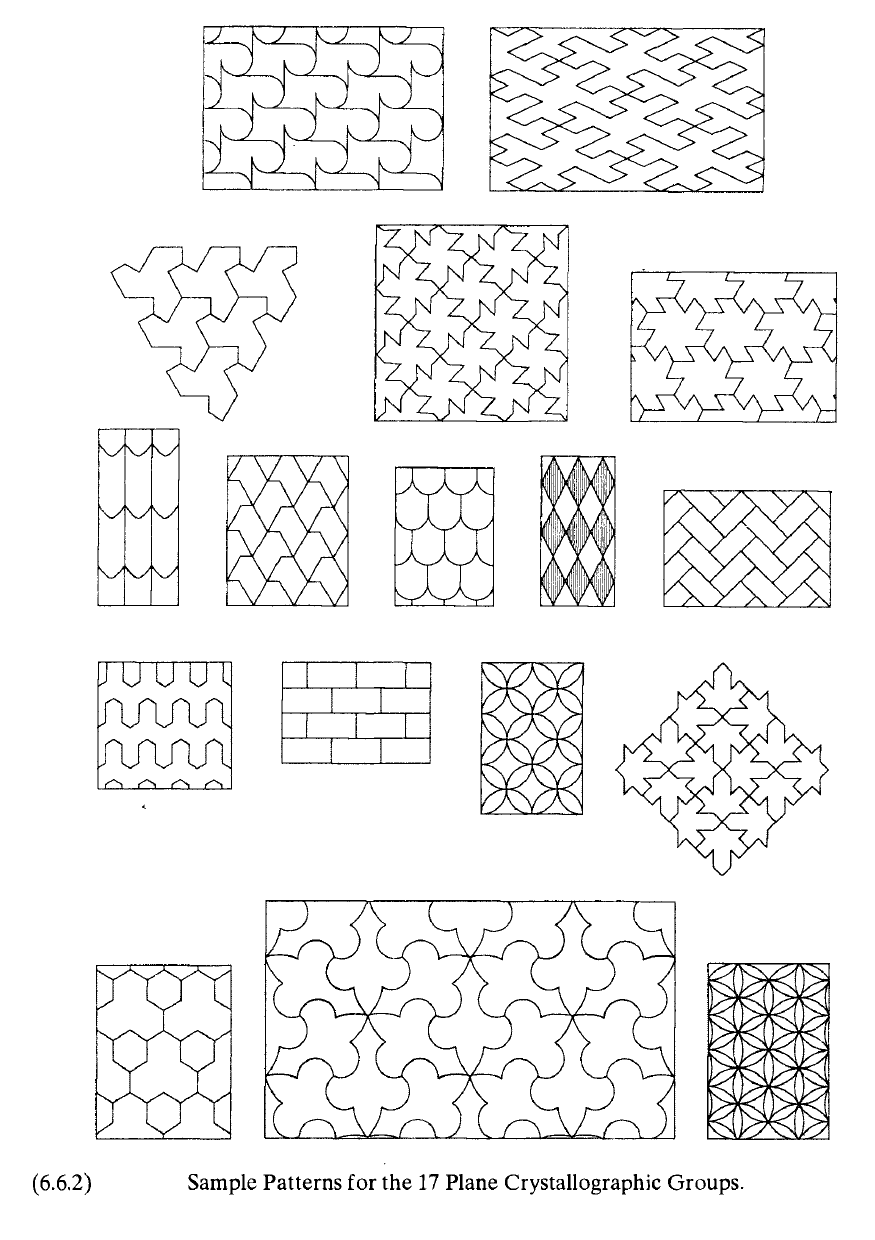
\includegraphics[height=0.77\textheight]{artin-algebra-2e-ch06-fig-6.6.2.png}\\[1pt]
{\tiny 图 6.6.2（原书印刷 p.~174 / PDF p.~186）；五行图案数 $2,3,5,4,3$，点群表见上一页。}
\end{frame}

% ---------------------------------------------------------- R2 14/21 G148 (下)
\begin{frame}[t]{四、随机复习 14/21：G148 十七个壁纸图案的点群（下）}
\scriptsize
\key{详解 (b)}：$L$ 是平移子群；“选坐标”即把原点平移到 $c$，也就是把每个 $g$ 换成 $t_c^{-1}gt_c$。写 $g(x)=Ax+b$，则
\[ t_c^{-1}gt_c:\quad b\longmapsto b+(A-I)c . \]
因 $AL=L$，条件“$G$ 在此坐标下作用于 $L$”即 $g(L)=L$ 对一切 $g$，等价于 $b\in L$。对旋转（$\theta\ne0$）：$A-I$ 可逆，总可解 $(A-I)c=-b$，把旋转中心放到格点。对镜射：$\operatorname{im}(A-I)$ 是垂直于镜轴的一维空间，只有该分量可被原点平移消去；沿轴分量 $b_\parallel$ 不可消去：
\[ b_\parallel=0\iff\text{真镜射};\qquad b_\parallel\ne0\iff\text{被迫滑移}. \]
故“能选到坐标使 $G$ 作用于 $L$”$\iff$ 每个点群反射都有真镜射提升 $\iff$ $G$ 是对称型 (symmorphic)。

\key{结论}：可选的 $13$ 型为
\[ p1,\ p2,\ pm,\ cm,\ pmm,\ cmm,\ p3,\ p3m1,\ p31m,\ p4,\ p4m,\ p6,\ p6m; \]
不可选的 $4$ 型为 $pg$（第 3 行第 2 个）、$pmg$（第 4 行第 1 个）、$pgg$（第 3 行末的人字纹）、$p4g$（第 4 行第 4 个）。

\key{验算（逐行读图，对应 (a)）}：第 1 行纯平移（$C_1$）与中心对称“Z”块（$C_2$）；第 2 行 $120^\circ/90^\circ/60^\circ$ 风车（$C_3,C_4,C_6$）；第 3 行前三个无 $2$ 重中心（$D_1$），菱形格与人字纹有（$D_2$）；第 4 行四瓣圆与斜向星有四重中心（$D_4$）；第 5 行末的六瓣花为 $D_6$。合计 $5$ 个 $C$ 型、$12$ 个 $D$ 型，共 $17$ 个图案。

\key{数值验算}：$pm$ 的 $r(x,y)=(-x,y)$ 有 $b=0$，取 $c=0$ 即可。$pg$ 的 $g(x,y)=(x+\tfrac12,-y)$：$A-I=\operatorname{diag}(0,-2)$，$(A-I)c=(0,-2c_2)$，故 $b+(A-I)c=(\tfrac12,-2c_2)$ 的沿轴分量恒为 $\tfrac12$，永不落入 $L=\mathbb Z^2$。程序核对：标准 $17$ 型的点群分配（$C_1,C_2,C_3,C_4,C_6$ 各 $1$ 个，$D_1^{\times3},D_2^{\times4},D_3^{\times2},D_4^{\times2},D_6$ 各若干）与上图的逐行计数一致；对称型 $13$ 个加非对称型 $4$ 个恰为 $17$。

\starpt 源注：(1) 原书图 6.6.2 无逐图标号，“行内点群”按图读出，$\{pm,pg,cm,\dots\}$ 的逐图符号是标准识别。(2) 笔记把第 3 行末的人字纹记作 $pmg$、第 4 行首记作 $pgg$；但人字纹即 Artin p.~173 明言“不含反射”的 brick pattern，应为 $pgg$；两者点群同为 $D_2$，不影响结论，仅符号对调。(3) 笔记的 \texttt{pg,qquad\ pmg} 漏反斜杠，应为 \texttt{pg,\textbackslash qquad\ pmg}。
\end{frame}

% ============================================================
% 分片 R3：四、随机复习 15/21 -- 21/21
% G113, G162, G178, G19, G110, G169, G25
% 只含 frame 环境；由 wrapper-R3.tex 包裹编译。
% ============================================================

% ---------------------------------------------------------- R3 15/21 G113
\begin{frame}[t]{四、随机复习 15/21：G113 具有平凡稳定化子的点（上）}
\label{ex:G113}
\pdfbookmark[2]{G113 具有平凡稳定化子的点}{bm:ex-G113}
\scriptsize
\begin{block}{\footnotesize 题面（\ex{G113}；Artin 2e, Ch.~6, §5, Ex.~5.9，印刷 p.~189 / PDF p.~201）}
Let $G$ be a discrete subgroup of $M$ whose translation group is not trivial. Prove that there is a point $p_0$ in the plane that is not fixed by any element of $G$ except the identity.
\end{block}
\key{思路}：非单位等距变换的不动集只能是空集、单点或直线；离散群的元素可数，而可数多个点与直线盖不住平面（取一条不平行于任何固定直线的直线）。

\key{详解（不动集的形状）}：由平面等距变换的分类（Artin 公式 (6.3.1)），非单位等距变换 $g$ 只有四类：旋转（绕中心，不动集为一点）、镜射（不动集为镜轴，一条直线）、平移与滑移反射（无不动点）。若 $g\ne1$ 有两个不动点，则它逐点固定过这两点的直线，从而是镜射。故
\[ \operatorname{Fix}(g)\in\{\varnothing,\ \text{一点},\ \text{一直线}\},\qquad g\ne 1. \]

\key{详解（$G$ 可数）}：注意 Artin 的“离散”定义 (6.5.1) 是“不含任意小的平移与旋转”，并非“$G$ 是 $M$ 的离散子集”，需要补一步论证。设 $\overline G\subseteq O_2$ 是点群（所有线性部分），$R=\overline G\cap SO_2$ 是旋转部分。由 (6.5.1)(ii)，$R$ 中非恒等元的旋转角绝对值 $\ge\varepsilon$，故 $R$ 是圆周群中的离散子群，从而是有限群；又 $|\overline G:R|\le2$，故 $\overline G$ 有限。平移子群 $L=\ker(G\to O_2)$ 由 (6.5.1)(i) 满足：非零 $v\in L$ 有 $|v|\ge\varepsilon$，故 $L$ 是 $\mathbb R^2$ 的离散子群，从而可数。于是
\[ G=\bigcup_{A\in\overline G} g_A L\quad(\text{有限并}),\qquad G\ \text{可数}. \]
\end{frame}

% ---------------------------------------------------------- R3 15/21 G113 (下)
\begin{frame}[t]{四、随机复习 15/21：G113 具有平凡稳定化子的点（下）}
\scriptsize
\key{详解（选点）}：令 $\mathcal B=\bigcup_{g\ne1}\operatorname{Fix}(g)$。固定直线至多可数条，其方向也至多可数，故可取一条直线 $\ell$，其方向不同于所有固定直线的方向。于是对每条固定直线 $L$，$\ell\cap L$ 至多一个点；点型不动集也各至多贡献一个点。因此 $\ell\cap\mathcal B$ 可数，而 $\ell$ 不可数，故存在
\[ p_0\in\ell\setminus\mathcal B. \]
按 $\mathcal B$ 的定义，对每个 $g\ne1$ 都有 $p_0\notin\operatorname{Fix}(g)$，即 $g(p_0)\ne p_0$，于是
\[ G_{p_0}=\{g\in G:g(p_0)=p_0\}=\{1\}. \qquad\square \]

\key{验算（$\mathbb Z^2\rtimes D_4$ 上的显式点）}：取 $G=\mathbb Z^2\rtimes D_4$（$p4m$ 型壁纸群：平移子群 $\mathbb Z^2\ne0$、点群 $D_4$ 八阶，故离散），取 $p_0=(0.1234,0.5678)$。对 $A\in D_4$、$b\in\mathbb Z^2$，
\[ A p_0+b=p_0\iff (A-I)p_0=-b\in\mathbb Z^2. \]
Python 逐一检查 $D_4$ 的 $8$ 个正交部分：只有 $A=I$ 且 $b=0$ 满足，故 $G_{p_0}=\{1\}$。

\key{结构注记}：离散群的三个基本量是平移群 $L$、点群 $\overline G$ 与 $\overline G$ 在 $L$ 上的作用；本题只用前两个。$L\ne0$ 的假设使图案是一维或二维的离散图案，但对可数性论证并不必要。

\starpt 易错：库内 G113 笔记的可数性论证直接使用了“$G$ 是 $M$ 的离散子集”；在 Artin 定义 6.5.1 下这一步需要“点群有限 $+$ 平移群离散”的补充（本帧已补出）。结论不受影响。
\end{frame}

% ---------------------------------------------------------- R3 16/21 G162
\begin{frame}[t]{四、随机复习 16/21：G162 正方形顶点的轨道\textendash{}陪集双射（上）}
\label{ex:G162}
\pdfbookmark[2]{G162 正方形顶点的轨道–陪集双射}{bm:ex-G162}
\scriptsize
\begin{block}{\footnotesize 题面（\ex{G162}；Artin 2e, Ch.~6, §8, Ex.~8.3，印刷 p.~191 / PDF p.~203；公式 (6.8.4) 在印刷 p.~179 / PDF p.~191）}
Exhibit the bijective map (6.8.4) explicitly, when $G$ is the dihedral group $D_4$ and $S$ is the set of vertices of a square.
\end{block}
\key{思路}：取一个顶点 $v_0$，其稳定化子 $H$ 是二阶反射群；把四个左陪集 $r^kH$ 分别送到顶点 $r^k(v_0)$。

\key{详解（(6.8.4) 的陈述）}：命题 6.8.4：设群 $G$ 作用在集合 $S$ 上，$s\in S$，$H$ 与 $O_s$ 分别为 $s$ 的稳定化子与轨道，则
\[ \epsilon:G/H\longrightarrow O_s,\qquad [aH]\longmapsto as \]
是双射，且与作用相容：$\epsilon(g[C])=g\,\epsilon([C])$。

\key{详解（本题设置）}：设 $D_4=\langle r,s\mid r^4=s^2=1,\ srs=r^{-1}\rangle$，其中 $r$ 是绕中心转 $90^\circ$，$s$ 是沿过 $v_0$ 的对角线的反射。记 $v_k=r^k(v_0)$（$k=0,1,2,3$）。$s$ 固定 $v_0$ 与 $v_2$，而顶点轨道大小为 $4$、$|D_4|=8$，故稳定化子二阶：
\[ H=\operatorname{Stab}(v_0)=\{1,s\}. \]
四个左陪集是
\[ H=\{1,s\},\quad rH=\{r,rs\},\quad r^2H=\{r^2,r^2s\},\quad r^3H=\{r^3,r^3s\}. \]
\end{frame}

% ---------------------------------------------------------- R3 16/21 G162 (下)
\begin{frame}[t]{四、随机复习 16/21：G162 正方形顶点的轨道\textendash{}陪集双射（下）}
\scriptsize
\key{详解（显式双射）}：于是 (6.8.4) 具体化为
\[ \Phi:D_4/H\longrightarrow S,\qquad \Phi(r^kH)=r^k(v_0)=v_k\qquad(k=0,1,2,3). \]
\textbf{良定义}：若 $aH=bH$，则 $b=ah$，$h\in H$，故 $b(v_0)=a(h(v_0))=a(v_0)$（$H$ 固定 $v_0$）。\textbf{单射}：若 $a(v_0)=b(v_0)$，则 $b^{-1}a\in H$，即 $aH=bH$。\textbf{满射}：每个 $v_k=r^k(v_0)$ 都在像中。故 $\Phi$ 是双射。

\key{验算（逐陪集列出并核对相容性）}：
\[ \Phi(H)=v_0,\quad \Phi(rH)=v_1,\quad \Phi(r^2H)=v_2,\quad \Phi(r^3H)=v_3. \]
相容性：对任意 $g\in D_4$ 与陪集 $C=aH$，
\[ \epsilon(g[C])=\epsilon([gaH])=ga(v_0)=g\bigl(a(v_0)\bigr)=g\,\epsilon([C]). \]
Python 以 $4$ 个顶点的置换实现 $D_4$：$|D_4|=8$，$|H|=2$，四个左陪集各 $2$ 元且并为 $D_4$；$\Phi$ 的值恰为四个顶点（双射），并对全部 $g$、$C$ 验证了 $\Phi(gC)=g\Phi(C)$。

\key{一般模式}：这正是“稳定化子同阶”的具体模型：$G/H\cong G s$，且每个顶点稳定化子都是二阶反射群；对另一个顶点 $v_1$ 重复即得该顶点的双射，二者由 $r$ 的平移相互转换。

\starpt 源注：库内 G162 笔记的两处显示公式有排版笔误（间距命令被写成了字面 qquad），数学内容不变；本帧按 (6.8.4) 重新写出该映射。
\end{frame}

% ---------------------------------------------------------- R3 17/21 G178
\begin{frame}[t]{四、随机复习 17/21：G178 最小忠实置换度（上）}
\label{ex:G178}
\pdfbookmark[2]{G178 最小忠实置换度}{bm:ex-G178}
\scriptsize
\begin{block}{\footnotesize 题面（\ex{G178}；Artin 2e, Ch.~6, §11, Ex.~11.7，印刷 p.~192 / PDF p.~204）}
For each of the following groups, find the smallest integer $n$ such that the group has a faithful operation on a set of order $n$: (a) $D_4$, (b) $D_6$, (c) the quaternion group $H$.
\end{block}
\key{思路}：在 $n$ 元集合上的忠实作用就是嵌入 $S_n$（不要求传递）；下界看阶与元素阶，上界给出具体作用。Artin 约定 $|D_m|=2m$，$H=Q_8$。

\key{详解 (a)}：$D_4$ 在正方形的 $4$ 个顶点上有忠实作用，故 $n\le4$。若 $n\le3$，则 $D_4\hookrightarrow S_n$，与 $|D_4|=8>|S_3|=6$ 矛盾。故
\[ n_{\min}(D_4)=4. \]

\key{详解 (b)}：$D_6=\langle x,y\mid x^6=y^2=1,\ yxy=x^{-1}\rangle$ 是 $12$ 阶六边形对称群。$x^3$ 是中心对合，$\langle x^2,y\rangle\cong D_3$，且
\[ D_6\cong D_3\times C_2\cong S_3\times C_2\qquad (x^3\ \text{与}\ \langle x^2,y\rangle\ \text{直积}). \]
让 $D_3$ 忠实作用于 $3$ 点、$C_2$ 作用于 $2$ 点，乘积作用在 $3+2=5$ 点上忠实，故 $n\le5$。若 $n\le4$，则 $D_6$ 嵌入 $S_4$；但 $S_4$ 只有一个 $12$ 阶子群 $A_4$，其元素阶只有 $1,2,3$，而 $x\in D_6$ 阶为 $6$，矛盾。故
\[ n_{\min}(D_6)=5. \]
\end{frame}

% ---------------------------------------------------------- R3 17/21 G178 (下)
\begin{frame}[t]{四、随机复习 17/21：G178 最小忠实置换度（下）}
\scriptsize
\key{详解 (c)}：$Q_8=\{\pm1,\pm i,\pm j,\pm k\}$。$Q_8$ 是哈密顿群：每个子群都正规；且每个非平凡子群都含唯一对合 $-1$。若 $Q_8$ 在 $n$ 点集合上作用，则各轨道大小整除 $8$。若某个轨道大小小于 $8$，其稳定化子 $H\ne1$，而 $H$ 正规，故该轨道的核为 $H\ni-1$。于是任何 $n<8$ 的作用都把 $-1$ 放进核，不忠实。另一方面，正则作用在 $8$ 点上忠实。故
\[ n_{\min}(Q_8)=8. \]

\key{验算（子群与核的穷举）}：用“忠实作用 = 若干轨道 $G/H_i$，$\bigcap_i \operatorname{core}(H_i)=1$”搜索最小总指数。程序结果：
\[ D_4:\ 10\ \text{个子群},\ n_{\min}=4;\quad D_6:\ 16\ \text{个子群},\ n_{\min}=5;\quad Q_8:\ 6\ \text{个子群},\ n_{\min}=8. \]
另核对：$S_4$ 的 $12$ 阶子群唯一（元素阶集 $\{1,2,3\}$，无 $6$ 阶元）；$Q_8$ 的 $5$ 个非平凡子群全部含 $-1$；$D_6$ 的中心为二阶 $\{1,x^3\}$，且在 $3+2=5$ 点上的作用给出 $12$ 个互异的置换。

\key{补充（(b) 的直接构造）}：$D_6$ 在“对顶点对”（$3$ 个点）上的作用核为 $\{1,x^3\}$；再附加 $k\bmod2$ 给出的 $C_2$ 作用（$2$ 个点），两核之交为 $\{1\}$，故 $5$ 点作用忠实。

\starpt 易错：$D_6$ 不是 $6$ 阶群！按 Artin 约定 $|D_6|=12$；其最小忠实度 $5$ 来自“$3+2$”的分解，而不是自然的 $6$ 顶点作用。另注意“在 $n$ 点上的作用”允许不传递。
\end{frame}

% ---------------------------------------------------------- R3 18/21 G19
\begin{frame}[t]{四、随机复习 18/21：G19 平面的线性反射（上）}
\label{ex:G19}
\pdfbookmark[2]{G19 平面的线性反射}{bm:ex-G19}
\scriptsize
\begin{block}{\footnotesize 题面（\ex{G19}；Artin 2e, Ch.~6, §3, Ex.~3.3，印刷 p.~188 / PDF p.~200）}
Prove that a linear operator on $\mathbb R^2$ is a reflection if and only if its eigenvalues are $1$ and $-1$, and the eigenvectors with these eigenvalues are orthogonal.
\end{block}
\key{思路}：镜射沿镜轴保留分量、沿垂直方向反转分量；反过来，正交特征向量在 $\mathbb R^2$ 中构成一组基，逐坐标读出这两个动作。

\key{详解（$\Rightarrow$）}：设 $T$ 是关于过原点直线 $L$ 的镜射。取 $0\ne u\in L$、$0\ne v\in L^\perp$，则 $T$ 固定 $L$ 上每个向量、反转 $L^\perp$ 上每个向量：
\[ T(u)=u,\qquad T(v)=-v. \]
故 $1,-1$ 是 $T$ 的特征值，对应的特征向量 $u,v$ 分别落在 $L$ 与 $L^\perp$，因此正交。$\square$

\key{详解（$\Leftarrow$）}：设 $T(u)=u$、$T(v)=-v$，其中 $u,v\ne0$ 且 $u\perp v$。$\mathbb R^2$ 中两个非零正交向量线性无关，故 $\{u,v\}$ 是一组基；任一 $x\in\mathbb R^2$ 有唯一表示 $x=au+bv$，由线性性
\[ T(x)=aT(u)+bT(v)=au-bv. \]
令 $L=\operatorname{span}(u)$，$L^\perp=\operatorname{span}(v)$；上式说明 $T$ 保留 $L$ 分量、反转 $L^\perp$ 分量，故 $T$ 是关于 $L$ 的镜射。$\square$

\key{所需标准结果}：特征值互异 $\Rightarrow$ 可对角化（此处两个特征值 $1\ne-1$），故两个特征空间之直和为 $\mathbb R^2$；这是第二方向把“特征值条件”转成“存在特征基”的依据。
\end{frame}

% ---------------------------------------------------------- R3 18/21 G19 (下)
\begin{frame}[t]{四、随机复习 18/21：G19 平面的线性反射（下）}
\scriptsize
\key{验算（正交特征基的具体例子）}：对随机角度 $\theta$，令 $M=R_\theta\operatorname{diag}(1,-1)R_\theta^{\,t}$。则
\[ \operatorname{eig}(M)=\{1,-1\},\qquad \text{特征向量正交},\qquad M^2=I, \]
且特征向量为 $u=(\cos\theta,\sin\theta)^t$（特征值 $1$，即镜轴方向）与 $v=(-\sin\theta,\cos\theta)^t$（特征值 $-1$）。反过来，任取单位正交 $u,v$，$T=uu^t-vv^t$ 满足 $T(u)=u$、$T(v)=-v$。

\key{反例（正交性不能去掉）}：取
\[ T=\begin{pmatrix}1&1\\0&-1\end{pmatrix},\qquad T\begin{pmatrix}1\\0\end{pmatrix}=\begin{pmatrix}1\\0\end{pmatrix},\quad T\begin{pmatrix}1\\-2\end{pmatrix}=\begin{pmatrix}-1\\2\end{pmatrix}. \]
于是 $T$ 的特征值为 $1,-1$，$T^2=I$，但特征向量 $(1,0)$ 与 $(1,-2)$ 不正交（内积为 $1$）。并且
\[ T^tT=\begin{pmatrix}1&1\\1&2\end{pmatrix}\ne I, \]
故 $T$ 不是正交变换，不是镜射，而是一个“斜对合”（沿 $L=\operatorname{span}(1,0)$ 方向保留、沿斜方向反演的仿射线性映射）。

\key{结论}：$T$ 是镜射 $\iff$ 存在正交特征基使矩阵为 $\operatorname{diag}(1,-1)$；换句话说，$T$ 是满足 $T^2=I$ 的对称正交变换。

\starpt 易错：题面中的“特征向量正交”是本质条件。缺了它，对合（$T^2=I$）与镜射不相等：$\mathbb R^2$ 中还有无穷多个斜对合。Python 核对：随机 $5$ 个轴向镜射均满足 $\{1,-1\}$ 与正交特征向量；反例矩阵满足 $T^2=I$ 但 $T^tT\ne I$。
\end{frame}

% ---------------------------------------------------------- R3 19/21 G110
\begin{frame}[t]{四、随机复习 19/21：G110 阶梯饰带的点群（上）}
\label{ex:G110}
\pdfbookmark[2]{G110 阶梯饰带的点群}{bm:ex-G110}
\scriptsize
\begin{block}{\footnotesize 题面（\ex{G110}；Artin 2e, Ch.~6, §5, Ex.~5.6，印刷 p.~188 / PDF p.~200）}
Let $G$ be the group of symmetries of the frieze pattern
\begin{center}
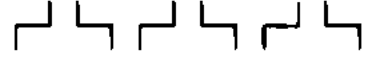
\includegraphics[width=0.44\textwidth]{artin-algebra-2e-ch06-ex-5.6-frieze.png}
\end{center}
Determine the point group $\overline G$ of $G$, and the index in $G$ of its subgroup of translations.
\end{block}
\key{思路}：图案由两种“阶梯”母题交替组成；最小平移 $t$ 跨两个母题，竖直镜面交换两种母题，水平方向只有“水平镜射 $+$ 半个周期平移”的滑移反射。点群取各对称的正交部分。

\key{详解（母题与平移）}：记相邻母题间距为 $u$。母题 $A$（左竖笔向下、右竖笔向上）与母题 $B$（左竖笔向上、右竖笔向下）交替排列，故平移 $u$ 把 $A$ 送到 $B$（形状不同），只有平移 $2u$ 使图案回到自身：
\[ t=t_{2u},\qquad L=\langle t\rangle\cong\mathbb Z,\qquad [G:L]=|\overline G|. \]

\key{详解（三个基本对称）}：设 $r$ 为关于水平中线的镜射。则
\[ g=t_u\circ r \]
把 $A(x)$ 送到 $B(x+u)$，故 $g\in G$ 是滑移反射，且 $g^2=t_{2u}=t$（$r$ 固定水平向量 $u$）。设 $s$ 为相邻母题间隙中点处的竖直镜射，则 $s$ 交换 $A$ 与 $B$。于是 $s\circ g$ 的正交部分为
\[ \operatorname{diag}(-1,1)\circ\operatorname{diag}(1,-1)=-I, \]
故 $s\circ g$ 是半转。综上，点群包含 $I,\ s,\ r,\ -I$。
\end{frame}

% ---------------------------------------------------------- R3 19/21 G110 (下)
\begin{frame}[t]{四、随机复习 19/21：G110 阶梯饰带的点群（下）}
\scriptsize
\key{详解（点群恰为四阶）}：对 $g\in G$ 与平移 $t_v\in L$，共轭给出 $g t_v g^{-1}=t_{Av}$（$A$ 为 $g$ 的正交部分），故 $A(L)=L$。而 $L=2u\mathbb Z$ 沿水平方向，故 $A e_1=\pm e_1$；这样的正交矩阵只有
\[ \overline G\subseteq\{\,I,\ \operatorname{diag}(-1,1),\ \operatorname{diag}(1,-1),\ -I\,\}. \]
四个都已实现（$I$ 由平移、$\operatorname{diag}(-1,1)$ 由 $s$、$\operatorname{diag}(1,-1)$ 由 $g$、$-I$ 由 $s\circ g$），故
\[ \overline G=\{I,s,r,-I\}\cong C_2\times C_2=D_2,\qquad |\overline G|=4. \]

\key{详解（指数）}：$G\to O_2$ 的核恰为平移子群 $L$（正交部分为 $I$ 的等距变换就是平移），故 $G/L\cong\overline G$，
\[ [G:L]=|\overline G|=4. \]
即每个对称唯一形如 $t^k,\ t^ks,\ t^kg,\ t^k(sg)$ 之一：$k\bmod2$ 定位置，是否含 $r$ 分量定方向。

\key{验算（逐段核对 $+$ 程序）}：取 $u=1.6$、横段长 $1$、竖笔长 $0.8$ 的整数模型（以 $0.1$ 为单位），周期 $P=2u=3.2$。程序对四个候选正交部分与相应平移量逐一检验图案不变性：四类都实现（点群 $4$ 阶）；纯水平镜射（平移量 $0$）不是对称，而滑移 $t_u\circ r$ 是；$g^2=t_{2u}$；水平平移只有 $P$ 的整数倍，故平移子群指数为 $4$。竖直镜轴位于母题间隙中点（如 $x=1.3=(1+1.6)/2$），相邻镜轴相距 $u$。

\starpt 易错：点群元素 $\operatorname{diag}(1,-1)$ 在 $G$ 中由滑移反射提升，而不是由水平镜射提升；“点群里有水平镜射”不等于“图案有水平镜面”。
\end{frame}

% ---------------------------------------------------------- R3 20/21 G169
\begin{frame}[t]{四、随机复习 20/21：G169 棒球接缝的对称群（上）}
\label{ex:G169}
\pdfbookmark[2]{G169 棒球接缝的对称群}{bm:ex-G169}
\scriptsize
\begin{block}{\footnotesize 题面（\ex{G169}；Artin 2e, Ch.~6, §9, Ex.~9.6，印刷 p.~192 / PDF p.~204）}
Identify the group of symmetries of a baseball, taking the seam (but not the stitching) into account and allowing orientation-reversing symmetries.
\end{block}
\key{思路}：球心置于原点，缝线是球面上的简单闭曲线（两块全等皮片的公共边界）。找出绕两“腰”轴的不当四分之一转 $a$ 与一条水平半转 $b$，验证 $bab=a^{-1}$；再用缝线的 $4$ 个曲率最大点给出 $|G|\le8$。

\key{详解（缝线的结构）}：缝线由两条全等弧组成，绕两“腰”的轴 $\ell$ 有半转 $h$；四个“发夹”点是缝线最靠近两极处。定义两个对称：
\begin{itemize}\setlength{\itemsep}{0pt}
\item $a$：绕 $\ell$ 转 $90^\circ$，再关于垂直于 $\ell$ 的赤道面反射。$\det a=-1$，$a^2=h$，故 $a^4=1$；
\item $b$：绕一条与 $\ell$ 垂直的水平轴作半转。$\det b=+1$，$b^2=1$，且 $b$ 反转 $a$ 的旋转方向：$bab=a^{-1}$。
\end{itemize}
于是 $\langle a,b\rangle$ 满足 $D_4$ 的表现，是 $8$ 阶二面体群：
\[ \langle a,b\rangle=\{1,a,a^2,a^3,b,ab,a^2b,a^3b\}\cong D_4\subseteq G. \]

\key{提示（为何允许反向）}：$a$ 与 $a^3$ 是反向对称；若只允许保向对称，$8$ 阶中只剩 $4$ 个（$1,h,b,a^2b$：三个半转加恒等），故题面明确“allowing orientation-reversing symmetries”是必要的。
\end{frame}

% ---------------------------------------------------------- R3 20/21 G169 (下)
\begin{frame}[t]{四、随机复习 20/21：G169 棒球接缝的对称群（下）}
\scriptsize
\key{详解（上界 $|G|\le8$）}：缝线的标准球面参数化（$0\le t\le4\pi$，取 $a_0=0.4$）为
\[ x=\sin w\cos\psi,\quad y=\sin w\sin\psi,\quad z=\cos w,\quad w=\tfrac\pi2-\bigl(\tfrac\pi2-a_0\bigr)\cos t,\quad \psi=\tfrac t2+a_0\sin2t. \]
对该模型，$a$ 与 $b$ 恰对应参数变换 $t\mapsto t+\pi$ 与 $t\mapsto\pi-t$，故确实保缝线。数值计算其曲率 $\kappa(t)$：全局最大恰在 $4$ 个点 $t=0,\pi,2\pi,3\pi$（值相同 $\approx2.4195$，次局部极大仅 $1.4614$）。曲率是等距不变量，故任何对称置换这 $4$ 个“发夹”点构成的集合 $E$。$E$ 的距离构型为“两对近点”：
\[ d=0.7788\ (\text{两对}),\qquad d=1.9227\ (\text{其余四组}), \]
其等距群 $\cong (C_2\times C_2)\rtimes C_2=D_4$ 为 $8$ 阶；且 $E$ 中三点与一点之差的行列式非零，故 $G$ 在 $E$ 上的作用忠实：
\[ |G|\le|\operatorname{Sym}(E)|=8. \]
结合已构造的 $8$ 阶子群，得 $G\cong D_4$。

\key{验算（参数化模型的数值核对）}：$\max|a\,r(t)-r(t+\pi)|\approx1.4\times10^{-15}$，$\max|b\,r(t)-r(\pi-t)|\approx7.8\times10^{-16}$；$8$ 个元素的像到缝线的距离 $\le3.3\times10^{-15}$；四点的等距群恰 $8$ 个置换；$a^4=b^2=1$、$bab=a^{-1}$、$|\langle a,b\rangle|=8$。保向子群 $\{1,h,b,a^2b\}\cong V_4$，指数 $2$。

\starpt 源注：库内 G169 笔记的结论（$G\cong D_4$，$|G|=8$）正确，但两处显示公式有排版笔误（间距命令被写成了字面 qquad）；本帧按独立推导重写，并补上“只取保向对称得 $V_4$”的对照。
\end{frame}

% ---------------------------------------------------------- R3 21/21 G25
\begin{frame}[t]{四、随机复习 21/21：G25 D10 的陪集与商群（上）}
\label{ex:G25}
\pdfbookmark[2]{G25 D10 的陪集与商群}{bm:ex-G25}
\scriptsize
\begin{block}{\footnotesize 题面（\ex{G25}；Artin 2e, Ch.~6, §4, Ex.~4.3，印刷 p.~188 / PDF p.~200）}
\textbf{(a)} Compute the left cosets of the subgroup $H=\{1,x^5\}$ in the dihedral group $D_{10}$.\\
\textbf{(b)} Prove that $H$ is normal and that $D_{10}/H$ is isomorphic to $D_5$.\\
\textbf{(c)} Is $D_{10}$ isomorphic to $D_5\times H$?
\end{block}
其中 $D_{10}=\langle x,y\mid x^{10}=1,\ y^2=1,\ yxy=x^{-1}\rangle$（Artin 的约定 $|D_{10}|=20$）。

\key{思路}：$H$ 由半转 $x^5$ 生成、是中心元，故左陪集即右陪集，每个陪集为 $\{a,ax^5\}$；(b) 从群表现读出商群；(c) 因 $5$ 为奇数，可取“奇偶分解”$K=\langle x^2,y\rangle$ 作直积因子。

\key{详解 (a)}：先由 (b) 知 $x^5\in Z(D_{10})$，故 $H\subseteq Z$，左、右陪集一致，每个陪集恰两个元素。把 $D_{10}$ 的 $20$ 个元素按 $x$ 的指数配对：
\[ x^kH=\{x^k,x^{k+5}\}\ (0\le k\le4),\qquad x^kyH=\{x^ky,x^{k+5}y\}\ (0\le k\le4). \]
这 $10$ 个二元子集互不相交，且 $10\cdot2=20=|D_{10}|$，故它们恰是全部左陪集。完整列表（各列 $k=0,1,2,3,4$）：
\begin{center}
\begin{tabular}{@{}lccccc@{}}
\toprule
$x^kH$ & $\{1,x^5\}$ & $\{x,x^6\}$ & $\{x^2,x^7\}$ & $\{x^3,x^8\}$ & $\{x^4,x^9\}$\\
$x^kyH$ & $\{y,x^5y\}$ & $\{xy,x^6y\}$ & $\{x^2y,x^7y\}$ & $\{x^3y,x^8y\}$ & $\{x^4y,x^9y\}$\\
\bottomrule
\end{tabular}
\end{center}

\key{详解 (b)}：$x^5$ 与 $x$ 交换，且
\[ yx^5y^{-1}=x^{-5}\cdot y y^{-1}=x^{-5}=x^5\quad(\text{用 }x^{10}=1), \]
故 $x^5\in Z(D_{10})$，$H\trianglelefteq D_{10}$。在商群中，$\bar x=xH$ 满足 $\bar x^5=x^5H=H$，$\bar y=yH$ 满足 $\bar y^2=H$，且
\[ \bar y\,\bar x\,\bar y^{-1}=x^{-1}H=\bar x^{-1}, \]
即商群满足 $D_5$ 的表现；又 $|D_{10}/H|=20/2=10$，故 $D_{10}/H\cong D_5$。
\end{frame}

% ---------------------------------------------------------- R3 21/21 G25 (下)
\begin{frame}[t]{四、随机复习 21/21：G25 D10 的陪集与商群（下）}
\scriptsize
\key{详解 (c)}：答案是“是”。令 $K=\langle x^2,y\rangle$。$x^2$ 的阶为 $5$，且 $yx^2y^{-1}=x^{-2}=(x^2)^{-1}$，故 $K$ 有 $D_5$ 的表现，$|K|=10$；$K$ 是 $2$ 次指数子群，故正规。$K$ 的旋转元为偶次幂 $x^{2j}$，而 $x^5$ 是奇次幂，故
\[ K\cap H=\{1\}. \]
又 $x=(x^2)^3x^5\in KH$（因 $(x^2)^3=x^6$，$x^6x^5=x^{11}=x$），而 $y\in K$，$x,y$ 生成 $D_{10}$，故 $KH=D_{10}$。$H\subseteq Z(D_{10})$ 与 $K$ 的元素交换，于是 $D_{10}$ 是 $K$ 与 $H$ 的内直积：
\[ D_{10}\cong K\times H\cong D_5\times H\cong D_5\times C_2. \]
等价地，$D_5=\langle a,b\rangle$、$C_2=\langle c\rangle$ 时，
\[ \varphi(x^ky^e)=\bigl(a^k b^e,\ c^{k}\bigr)\qquad(e\in\{0,1\}) \]
是双射同态：$k\bmod10\mapsto(k\bmod5,k\bmod2)$ 由中国剩余定理是双射（$\gcd(5,2)=1$），逐项验证可知 $\varphi$ 保持乘法。

\key{验算（Python 枚举）}：以 $20$ 个元素的置换表示枚举：左陪集恰 $10$ 个、每个 $2$ 元；$Z(D_{10})=\{1,x^5\}$；商群中 $xH$ 阶 $5$、$yH$ 阶 $2$、$yH\,xH\,yH=(xH)^{-1}$ 且商群非交换，故 $\cong D_5$；$K=\langle x^2,y\rangle$ 阶 $10$、$K\cap H=\{1\}$、$|KH|=20$；显式 $\varphi$ 是双射同态，故 $D_{10}\cong D_5\times C_2$。反射型陪集用 $x^ky\cdot x^5=x^{k-5}y=x^{k+5}y$ 核对。

\key{注记（左陪集即右陪集）}：因 $H\subseteq Z(D_{10})$，左右陪集集合相同；一般地 $H\trianglelefteq G$ 当且仅当左右陪集集合一致。每个陪集 $\{a,ax^5\}$ 的两元素恰好相差半转 $x^5$，故商群元素可写成 $\bar x^i$ 与 $\bar x^i\bar y$（$0\le i\le4$）。计数核对：
\[ |D_{10}|=|H|\cdot|D_{10}/H|=2\cdot10=20=|D_5\times H|. \]

\starpt 易错：一般地 $D_{2m}\cong D_m\times C_2\iff m$ 为奇数（取半转 $x^m$ 生成的中央 $C_2$，再用奇偶分解）；$m$ 偶时分裂失败（如 $D_4\not\cong D_2\times C_2$）。本题 $m=5$ 为奇数，故 (c) 的答案是“是”。
\end{frame}

% ============================================================
% frag-S1.tex : Systematic Progress k = 1..7
% G247, LA308, G248, G249, G250, G251, G252 (Artin 2e, Ch. 7, §10--§11)
% Wrapped by wrapper-S1.tex; contains frames only.
% ============================================================

% ---------------------------------------------------------- S1/21 G247
\begin{frame}[t]{五、系统推进 1/21：G247 经典等距群的换位子群（上）}
\label{ex:G247}
\pdfbookmark[1]{五、系统推进（21 题）}{bm:sys}
\pdfbookmark[2]{G247 经典等距群的换位子群}{bm:ex-G247}
\scriptsize
\begin{block}{\footnotesize 题面（\ex{G247}；Artin 2e, Ch.~7, §10, Ex.~10.8，印刷 p.~226 / PDF p.~238）}
Determine the commutator subgroups (Exercise 10.7) of the following groups: \textbf{(a)} $SO_2$, \textbf{(b)} $O_2$, \textbf{(c)} the group $M$ of isometries of the plane, \textbf{(d)} $S_n$, \textbf{(d)} $SO_3$.
\end{block}
\starpt 源注：原书把 $S_n$ 与 $SO_3$ 两项都印作 \textbf{(d)}（印刷 p.~226 / PDF p.~238）。此处照录；按顺序末项逻辑上应为 (e)。

\key{思路}：$[G,G]$ 是使 $G/[G,G]$ 交换的最小正规子群。先用 $\det$ 或定向同态给出上界 $[G,G]\subseteq\ker$，再用与反射的交换子构造反向包含；$SO_3$ 用两个半周转的交换子给出全部旋转。约定 $[a,b]=aba^{-1}b^{-1}$。

\key{(a) $[SO_2,SO_2]=1$}：平面旋转 $r_\theta r_\varphi=r_{\theta+\varphi}=r_\varphi r_\theta$，$SO_2$ 交换，故换位子群平凡。

\key{(b) $[O_2,O_2]=SO_2$}：$\det:O_2\to\{\pm1\}$ 是满的交换商，故 $[O_2,O_2]\subseteq SO_2$。另一方面取反射 $s=\operatorname{diag}(1,-1)$，由 $sr_\theta s^{-1}=r_{-\theta}$ 得
\[ [s,r_\theta]=s r_\theta s^{-1}r_\theta^{-1}=r_{-2\theta}. \]
$\theta\mapsto-2\theta$ 是圆周到自身的满射，故每个旋转都是换位子，$SO_2\subseteq[O_2,O_2]$，等号成立。
\end{frame}

% ---------------------------------------------------------- S1/21 G247
\begin{frame}[t]{五、系统推进 1/21：G247 经典等距群的换位子群（下）}
\scriptsize
\key{(c) $[M,M]=M^+=\mathbb R^2\rtimes SO_2$}：把等距写成 $f(x)=Ax+b$，$A\in O_2$，乘法为 $(A,b)(C,d)=(AC,Ad+b)$。定向同态 $\varepsilon(f)=\det A$ 给出交换商 $M/M^+\cong C_2$，故 $[M,M]\subseteq M^+$。取以过原点直线为轴的反射 $s=(S,0)$（$S^2=I$，$S\in O_2$）与平移 $t_v=(I,v)$，则 $s^{-1}=s$ 且
\[ s\,t_v\,s^{-1}=(I,Sv),\qquad [s,t_v]=s t_v s^{-1}t_v^{-1}=(I,\,Sv-v). \]
$S=\operatorname{diag}(1,-1)$ 时 $Sv-v=-2v_2e_2$，$S=\operatorname{diag}(-1,1)$ 时 $Sv-v=-2v_1e_1$，故全部平移属于 $[M,M]$。又 $[s,r_\theta]=s r_\theta s^{-1}r_\theta^{-1}=(R_{-2\theta},0)$ 给出全部旋转。于是 $M^+\subseteq[M,M]$，故 $[M,M]=M^+$；特别地 $[M,M]\neq M$。

\key{(d) $[S_n,S_n]=A_n$}：$\operatorname{sgn}:S_n\to\{\pm1\}$ 给出 $[S_n,S_n]\subseteq A_n$。$n\ge3$ 时 $A_n$ 由三循环生成，而
\[ [(12),(23)]=(12)(23)(12)(23)=(132), \]
共轭后得到全部三循环，故 $A_n\subseteq[S_n,S_n]$。$n=2$ 时 $S_2$ 交换，两边都是 $1$。

\key{(d) $[SO_3,SO_3]=SO_3$}：设 $A,B$ 分别是绕单位向量 $u,v$ 的半周转（转角 $\pi$），$u,v$ 夹角为 $\varphi$。两个半周转的复合是绕 $u\times v$、转角 $2\varphi$ 的旋转，且 $A,B$ 都是对合，故
\[ [A,B]=ABA^{-1}B^{-1}=ABAB=(AB)^2=\text{绕 }u\times v\text{ 转角 }4\varphi\text{ 的旋转}. \]
给定任意旋转 $r_\theta$，取其轴 $w$，任取 $u\perp w$，令 $v$ 为 $u$ 绕 $w$ 转 $\theta/4$ 所得向量，则 $[A,B]=r_\theta$。故每个旋转都是换位子，$[SO_3,SO_3]=SO_3$（$SO_3$ 完美）。

\key{验算}：$[s,r_{\pi/2}]=r_{-\pi}$（$O_2$ 中的半周旋转）；$[s,t_{(0,1)}]=(I,-2e_2)$（$M$ 中，取 $S=\operatorname{diag}(1,-1)$）；$[(12),(23)]=(132)\in A_4$（$S_4$ 中）。由 $M/M^+\cong C_2$ 知 $[M,M]$ 真小于 $M$，与 $SO_3$ 完美的结论形成对照。
\end{frame}

% ---------------------------------------------------------- S2/21 LA308
\begin{frame}[t]{五、系统推进 2/21：LA308 有限 Heisenberg 群的中心、换位子与元素阶（上）}
\label{ex:LA308}
\pdfbookmark[2]{LA308 有限 Heisenberg 群的中心、换位子与元素阶}{bm:ex-LA308}
\scriptsize
\begin{block}{\footnotesize 题面（\ex{LA308}；Artin 2e, Ch.~7, §10, Ex.~10.9，印刷 p.~226 / PDF p.~238）}
Let $G$ denote the group of $3\times3$ upper triangular matrices with diagonal entries equal to 1 and with entries in the field $\mathbb F_p$. For each prime $p$, determine the center, the commutator subgroup (Exercise 10.6), and the orders of the elements of $G$.
\end{block}
\starpt 源注：题面的“对角元为 1 的上三角矩阵”即对角为 1、其上方三个位置任意的单位上三角群，也就是 $p^3$ 阶 Heisenberg 群 $UT_3(\mathbb F_p)$；笔记中改写为“upper unitriangular”是等价澄清。
\key{思路}：把矩阵编码成三元组 $g(a,b,c)$，直接算乘法与换位子；中心与换位子都由 $ab'-a'b$ 读出；元素阶用乘法公式的归纳式（二项式律）。

\key{记号与乘法}：令
\[ g(a,b,c)=\begin{pmatrix}1&a&c\\0&1&b\\0&0&1\end{pmatrix},\qquad a,b,c\in\mathbb F_p, \]
则 $|G|=p^3$。直接相乘得
\[ g(a,b,c)\,g(a',b',c')=g\bigl(a+a',\ b+b',\ c+c'+ab'\bigr), \]
从而 $g(a,b,c)^{-1}=g(-a,-b,-c+ab)$。

\key{中心}：由上式算得交换子只依赖 $a,b,a',b'$：
\[ [g(a,b,c),\,g(a',b',c')]=g(0,0,\,ab'-a'b). \]
于是 $g(a,b,c)\in Z(G)\iff ab'-a'b=0$ 对一切 $a',b'$ 成立；分别取 $(a',b')=(0,1)$、$(1,0)$ 得 $a=0$、$b=0$，故
\[ Z(G)=\{g(0,0,c):c\in\mathbb F_p\}\cong C_p. \]
\end{frame}

% ---------------------------------------------------------- S2/21 LA308
\begin{frame}[t]{五、系统推进 2/21：LA308 有限 Heisenberg 群的中心、换位子与元素阶（下）}
\scriptsize
\key{换位子群}：换位子 $g(0,0,ab'-a'b)$ 中 $ab'-a'b$ 取遍 $\mathbb F_p$（取 $a=1,b'=t,a'=b=0$ 得 $t$），所以换位子集合就是 $\{g(0,0,t)\}$；它是子群，于是
\[ [G,G]=\{g(0,0,t):t\in\mathbb F_p\}=Z(G)\cong C_p. \]
又 $G$ 非交换且 $G/Z(G)\cong C_p^2$，故 $G$ 是 extraspecial $p$-群：$1\to C_p\to G\to C_p^2\to1$，换位子配对 $(a,b)\wedge(a',b')=ab'-a'b$ 非退化。

\key{元素阶}：由乘法公式归纳得（左边 $n$ 个 $g$ 相乘）
\[ g(a,b,c)^n=g\Bigl(na,\ nb,\ nc+\binom n2 ab\Bigr). \]
$p$ 为奇素数时 $\binom p2=\frac{p(p-1)}2$ 被 $p$ 整除，故 $g(a,b,c)^p=g(0,0,0)=1$：每个元素的阶整除 $p$，非单位元阶恰为 $p$。$p=2$ 时
\[ g(a,b,c)^2=g(0,0,ab), \]
故 $a=b=1$ 的两个元素阶为 $4$，其余非单位元阶为 $2$。

\key{验算}：$p=3$：$|G|=27$，$|Z|=|[G,G]|=3$，阶谱 $1\!:\!1,\ 3\!:\!26$。$p=5$：$|G|=125$，阶谱 $1\!:\!1,\ 5\!:\!124$。$p=2$：$|G|=8$，阶谱 $1\!:\!1,\ 2\!:\!5,\ 4\!:\!2$。以上由 Python 穷举 $p=2,3,5$ 的全部 $|G|\le125$ 个元素独立核对，并逐对验证换位子公式 $ab'-a'b$。
\end{frame}

% ---------------------------------------------------------- S3/21 G248
\begin{frame}[t]{五、系统推进 3/21：G248 秩二自由群中一个换位子的正规闭包}
\label{ex:G248}
\pdfbookmark[2]{G248 秩二自由群中一个换位子的正规闭包}{bm:ex-G248}
\scriptsize
\begin{block}{\footnotesize 题面（\ex{G248}；Artin 2e, Ch.~7, §10, Ex.~10.10，印刷 p.~226 / PDF p.~238）}
Let $\mathcal F$ be the free group on $x$, $y$ and let $\mathcal R$ be the smallest normal subgroup containing the commutator $xyx^{-1}y^{-1}$.
\textbf{(a)} Show that $x^2y^2x^{-2}y^{-2}$ is in $\mathcal R$.
\textbf{(b)} Prove that $\mathcal R$ is the commutator subgroup (Exercise 10.7) of $\mathcal F$.
\end{block}
\key{思路}：$\mathcal R$ 是正规闭包，故 $\mathcal F/\mathcal R=\langle x,y\mid [x,y]\rangle$ 交换。交换性一方面让指数和为 $0$ 的字落到 $\mathcal R$ 里；另一方面给出 $[\mathcal F,\mathcal F]\subseteq\mathcal R$，而反方向由“$\mathcal R$ 最小”直接得到。

\key{(a)}：在商群 $\mathcal F/\mathcal R$ 中 $\bar x\bar y=\bar y\bar x$，于是
\[ \bar x^2\bar y^2\bar x^{-2}\bar y^{-2}=\bar x^2\bar x^{-2}\,\bar y^2\bar y^{-2}=1, \]
即 $x^2y^2x^{-2}y^{-2}\in\ker(\mathcal F\twoheadrightarrow\mathcal F/\mathcal R)=\mathcal R$。

\key{(b)}：设 $\pi:\mathcal F\to\mathcal F/\mathcal R$。
\begin{itemize}
\item $\mathcal R\subseteq[\mathcal F,\mathcal F]$：$[\mathcal F,\mathcal F]$ 是正规子群，且含换位子 $xyx^{-1}y^{-1}$（即生成元之间的 $[x,y]$）；$\mathcal R$ 是含该元的最小正规子群，故 $\mathcal R\subseteq[\mathcal F,\mathcal F]$。
\item $[\mathcal F,\mathcal F]\subseteq\mathcal R$：$\mathcal F/\mathcal R$ 交换，故一切换位子 $[u,v]$ 在 $\pi$ 下映为 $1$，即 $[\mathcal F,\mathcal F]\subseteq\ker\pi=\mathcal R$。
\end{itemize}
因此 $\mathcal R=[\mathcal F,\mathcal F]$。由自由群泛性质，$\mathcal F/[\mathcal F,\mathcal F]\cong\mathbb Z^2$（$x,y$ 映为两组基，无其它关系），故 $\mathcal F/\mathcal R\cong\mathbb Z^2$。

\key{验算（显式分解）}：令 $c=[x,y]$。用恒等式 $[u,vw]=[u,v]\,v[u,w]v^{-1}$ 与 $[uv,w]=u[v,w]u^{-1}[u,w]$，取 $u=x^2$、$w=y^2$：
\[ x^2y^2x^{-2}y^{-2}=[x^2,y^2]=\bigl(x\,[x,y^2]\,x^{-1}\bigr)[x,y^2],\qquad [x,y^2]=c\,(ycy^{-1}). \]
右端是 $c=[x,y]$ 的共轭之积，显式落在正规闭包 $\mathcal R$ 中。该展开恒等式已在 $5$ 组随机 $S_6$ 元素上程序验证。
\end{frame}

% ---------------------------------------------------------- S4/21 G249
\begin{frame}[t]{五、系统推进 4/21：G249 补全例 7.11.8 的塌缩（上）}
\label{ex:G249}
\pdfbookmark[2]{G249 补全例 7.11.8 的塌缩}{bm:ex-G249}
\scriptsize
\begin{block}{\footnotesize 题面（\ex{G249}；Artin 2e, Ch.~7, §11, Ex.~11.1，印刷 p.~226 / PDF p.~238）}
Complete the proof that the group given in Example 7.11.8 is cyclic of order 3.
\end{block}
\key{背景}：Example 7.11.8（印刷 p.~219 / PDF p.~231）取 $G=\langle x,y\mid x^3,\ y^3,\ yxyxy\rangle$ 与 $H=\langle y\rangle$，用 Todd--Coxeter 表证明 $H=G$。该表的两步关键（原书原话）：
\begin{itemize}
\item 在 $yxyxy$ 的表中，第一行从左读得 $2\xrightarrow{y}3$，第二行从左读得 $2\xrightarrow{y}2$，故 $2=3$；
\item 再由 $xxx$ 的表得 $2=1$：只剩一个指标，于是 $H=G$。
\end{itemize}
所以陪集表只推出 $G=\langle y\rangle$ 且 $y^3=1$，即“循环、阶整除 $3$”。题目要求补的正是剩下的那一步。

\key{思路}：表本身给不出 $y\neq1$。两条独立途径补全：(i) 直接由关系式化简出 $x=1$，再证 $y\neq1$；(ii) 构造满同态 $G\twoheadrightarrow C_3$。

\key{补全 (i)：直接塌缩}：由 $yxyxy=1$，两边左乘 $y^{-1}$、右乘 $y^{-1}$：
\[ xyx=y^{-1}\cdot1\cdot y^{-1}=y^{-2}=y. \]
再两边左乘 $x^{-1}$ 得 $yx=x^{-1}y$，即
\[ y^{-1}xy=x^{-1};\qquad\text{共轭 }y^{-1}\text{ 把 }x\text{ 取逆}. \]
但 $y^3=1$，故共轭 $y^{-1}$ 对应自同构的阶整除 $3$；反演 $x\mapsto x^{-1}$ 的阶为 $2$，除非它把 $x$ 固定。两者互素（$3\nmid2$），故共轭作用平凡：
\[ x=x^{-1}\ \Longrightarrow\ x^2=1;\qquad x^3=1\ \Longrightarrow\ x=1. \]
于是 $G=\langle y\rangle$、$y^3=1$。
\end{frame}

% ---------------------------------------------------------- S4/21 G249
\begin{frame}[t]{五、系统推进 4/21：G249 补全例 7.11.8 的塌缩（下）}
\scriptsize
\key{补全 (ii)：满同态到 $C_3$}：设 $\omega\in C_3$ 为生成元。令 $x\mapsto1$、$y\mapsto\omega$，则三个关系式在 $C_3$ 中成立：
\[ 1^3=1,\qquad \omega^3=1,\qquad \omega\cdot1\cdot\omega\cdot1\cdot\omega=\omega^3=1. \]
由自由群泛性质，该指派诱导同态 $\varphi:G\to C_3$；因 $\varphi(y)=\omega$ 生成 $C_3$，$\varphi$ 是满射。结合表中得到的 $|G|\le3$：
\[ 3=|C_3|\le|G|\le3\ \Longrightarrow\ G\cong C_3. \]

\key{说明 (i) 与 (ii) 的关系}：(i) 给出 $x=1$，即 $G$ 是 $C_3$ 的商；(ii) 说明这个商恰为 $C_3$（$y$ 不塌缩）。原书在 Example 7.11.8 末尾直接写“cyclic group of order 3”，其隐含步骤正是 $y\neq1$；表只用到 $y^3=1$。

\key{验算}：Todd--Coxeter 独立重算：以 $H=\langle y\rangle$ 为子群枚举，恰得 $1$ 个陪集（本作者实现的小枚举器在 $x^3=1$ 上返回 $3$、在本例上返回 $1$，说明算法正确闭合）。$C_3$ 模型 $x=1,\ y=\omega$ 满足全部关系，故三个关系式不能推出 $y=1$。\starpt 源注：原书此处自带警告“Care is essential when constructing such a table. Any mistake will cause the operation to collapse”，题 11.1 正是要求把“塌缩到循环”补成“恰为 3 阶”。
\end{frame}

% ---------------------------------------------------------- S5/21 G250
\begin{frame}[t]{五、系统推进 5/21：G250 12 阶与 21 阶表现的 Todd–Coxeter 计数（上）}
\label{ex:G250}
\pdfbookmark[2]{G250 12 阶与 21 阶表现的 Todd–Coxeter 计数}{bm:ex-G250}
\scriptsize
\setlength{\parskip}{0pt}
\begin{block}{\footnotesize 题面（\ex{G250}；Artin 2e, Ch.~7, §11, Ex.~11.2，印刷 p.~226 / PDF p.~238）}
Use the Todd-Coxeter algorithm to show that the group defined by the relations (7.8.2) has order 12 and that the group defined by the relations (7.7.8) has order 21.
\end{block}
\key{两个表现}：(7.8.2) 见 Theorem 7.8.1 的 Case 3a（印刷 p.~209 / PDF p.~221），(7.7.8) 见 21 阶群分类的 Case 2（印刷 p.~206 / PDF p.~218）：
\[ (7.8.2)\quad G_{12}=\langle x,y\mid x^4=y^3=1,\ xy=y^2x\rangle, \]
\[ (7.7.8)\quad G_{21}=\langle x,y\mid x^7=y^3=1,\ yx=x^2y\rangle. \]
\key{思路}：取 $H=\langle x\rangle$ 枚举右陪集。由 $x^4=1$（或 $x^7=1$）得 $|H|\le4$（或 $\le7$）；若恰有 $3$ 个陪集，则 $|G|\le12$（或 $\le21$）。再用具体矩阵/置换模型给出同阶商群，上下界相合。

\key{$G_{12}$：$H=\langle x\rangle$ 的陪集表}：由 $xy=y^2x$ 得 $xyx^{-1}=y^2$，故 $\langle y\rangle\triangleleft G_{12}$，$G_{12}=\langle y\rangle\langle x\rangle$，右陪集 $H,Hy,Hy^2$；$y$ 循环置换三者，$x$ 固定 $H$ 并交换另两个：
\[ \begin{array}{c|cccc}
 & x & x^{-1} & y & y^{-1}\\\hline
1 & 1 & 1 & 2 & 3\\
2 & 3 & 3 & 3 & 1\\
3 & 2 & 2 & 1 & 2
\end{array} \]
逐字扫描 $x^4$、$y^3$、$xyx^{-1}y^{-2}$ 各行均闭合（如行 $2$ 上的 $x$ 循环 $2\to3\to2\to3\to2$），故 $[G_{12}:H]=3$、$|G_{12}|\le12$。

\key{下界（矩阵模型）}：取 $\omega=e^{2\pi i/3}$，
\[ x=\begin{pmatrix}0&-1\\1&0\end{pmatrix},\qquad y=\begin{pmatrix}\omega&0\\0&\omega^2\end{pmatrix}, \]
则 $x^4=y^3=1$、$xy=y^2x$，且 $\langle x,y\rangle$ 的阶为 $12$（Python 矩阵枚举确认）。故 $|G_{12}|=12$。
\end{frame}

% ---------------------------------------------------------- S5/21 G250
\begin{frame}[t]{五、系统推进 5/21：G250 12 阶与 21 阶表现的 Todd–Coxeter 计数（下）}
\scriptsize
\key{$G_{21}$：$H=\langle x\rangle$ 的陪集表}：由 $yx=x^2y$ 得 $yxy^{-1}=x^2$，故 $\langle x\rangle\triangleleft G_{21}$，$G_{21}=\langle x\rangle\langle y\rangle$，右陪集为 $H,Hy,Hy^2$。此时 $x$ 固定每个陪集（$x\in H$），$y$ 循环置换：
\[ \begin{array}{c|cccc}
 & x & x^{-1} & y & y^{-1}\\\hline
1 & 1 & 1 & 2 & 3\\
2 & 2 & 2 & 3 & 1\\
3 & 3 & 3 & 1 & 2
\end{array} \]
扫描 $x^7$、$y^3$、$yxy^{-1}x^{-2}$ 均闭合，得 $[G_{21}:H]=3$、$|G_{21}|\le3\cdot7=21$。

\key{下界（仿射模型）}：在 $\mathbb F_7$ 上令 $x:t\mapsto t+1$、$y:t\mapsto2t$。$x$ 是 $7$-循环；由 $2^3\equiv1\pmod7$ 得 $y^3=1$；又
\[ yxy^{-1}(t)=y\bigl(x(2^{-1}t)\bigr)=y(2^{-1}t+1)=t+2=x^2(t), \]
即 $yxy^{-1}=x^2$，等价于 $yx=x^2y$。$21$ 个映射 $t\mapsto at+b$（$a\in\langle2\rangle=\{1,2,4\}$，$b\in\mathbb F_7$）两两不同且对复合封闭，故模型群阶为 $21$（Python 置换枚举确认）。因此 $|G_{21}|=21$。

\key{验算}：$G_{12}$ 的矩阵模型中 $x$ 阶 $4$、$y$ 阶 $3$；$G_{21}$ 的仿射模型中 $x$ 阶 $7$、$y$ 阶 $3$。两处上界 $12$、$21$ 都与模型阶相等。$G_{12}\cong C_3\rtimes C_4$（$x$ 对 $y$ 的作用为平方，即非平凡 $C_2$），$G_{21}\cong C_7\rtimes C_3$（$y$ 对 $x$ 的作用为平方），都非交换。
\end{frame}

% ---------------------------------------------------------- S6/21 G251
\begin{frame}[t]{五、系统推进 6/21：G251 十个双生成元表现的 Todd–Coxeter 枚举（上）}
\label{ex:G251}
\pdfbookmark[2]{G251 十个双生成元表现的 Todd–Coxeter 枚举}{bm:ex-G251}
\scriptsize
\begin{block}{\footnotesize 题面（\ex{G251}；Artin 2e, Ch.~7, §11, Ex.~11.3，印刷 p.~226 / PDF p.~238）}
Use the Todd-Coxeter Algorithm to analyze the group generated by two elements $x$, $y$, with the following relations. Determine the order of the group and identify the group if you can:
\textbf{(a)} $x^2=y^2=1$, $xyx=yxy$;\ \textbf{(b)} $x^3=y^3=1$, $xyx=yxy$;\ \textbf{(c)} $x^4=y^2=1$, $xyx=yxy$;\ \textbf{(d)} $x^4=y^4=x^2y^2=1$;
\textbf{(e)} $x^3=1$, $y^2=1$, $yxyxy=1$;\ \textbf{(f)} $x^3=y^3=yxyxy=1$;\ \textbf{(g)} $x^4=1$, $y^3=1$, $xy=y^2x$;\ \textbf{(h)} $x^7=1$, $y^3=1$, $yx=x^2y$;
\textbf{(i)} $x^{-1}yx=y^{-1}$, $y^{-1}xy=x^{-1}$;\ \textbf{(j)} $y^3=1$, $x^2yxy=1$.
\end{block}
\key{思路}：先用辫关系 $xyx=yxy$ 化简 (a)--(c)，再用换位/共轭关系把群写成半直积或循环群；唯一无穷的是 (d)，用无限二面体商群证明。下表汇总十个结果，下一帧给出关键推导与验算。
\begin{center}
\renewcommand{\arraystretch}{1.18}
\begin{tabular}{@{}c l c l@{}}
\toprule
 & 关系 & $|G|$ & 识别 \\\midrule
(a) & $x^2=y^2=1,\ xyx=yxy$ & $6$ & $S_3$（二面体 $D_3$）\\
(b) & $x^3=y^3=1,\ xyx=yxy$ & $24$ & $SL_2(\mathbb F_3)$（计算值）\\
(c) & $x^4=y^2=1,\ xyx=yxy$ & $6$ & $S_3$（表迫使 $x^2=1$）\\
(d) & $x^4=y^4=x^2y^2=1$ & $\infty$ & $C_4*_{C_2}C_4$\\
(e) & $x^3=1,\ y^2=1,\ yxyxy=1$ & $1$ & 平凡群\\
(f) & $x^3=y^3=yxyxy=1$ & $3$ & $C_3$\\
(g) & $x^4=1,\ y^3=1,\ xy=y^2x$ & $12$ & $C_3\rtimes C_4$\\
(h) & $x^7=1,\ y^3=1,\ yx=x^2y$ & $21$ & $C_7\rtimes C_3$\\
(i) & $x^{-1}yx=y^{-1},\ y^{-1}xy=x^{-1}$ & $8$ & $Q_8$\\
(j) & $y^3=1,\ x^2yxy=1$ & $9$ & $C_9$\\
\bottomrule
\end{tabular}
\end{center}
\end{frame}

% ---------------------------------------------------------- S6/21 G251
\begin{frame}[t]{五、系统推进 6/21：G251 十个双生成元表现的 Todd–Coxeter 枚举（下）}
\scriptsize
\key{关键推导}：
\begin{itemize}
\item (a) 由 $xyx=yxy$ 左乘 $x$ 得 $yx=(xy)^2$，于是 $(xy)^3=xy\,yx=x^2=1$；故 $G$ 是二面体 $D_3$ 的商，而 $S_3$ 模型 $x=(12),y=(23)$ 达到 $6$。
\item (c) 由关系得 $(xy)^2=(xyx)y=(yxy)y=yxy^2=yx$，故 $(yx)^2=y(xyx)=y(yxy)=y^2xy=xy$。于是 $yxyx=xy$，右乘 $x^{-1}$ 得 $yxy=xyx^{-1}$；与 $yxy=xyx$ 比较得 $x=x^{-1}$，即 $x^2=1$。又 $(xy)^3=(xy)(yx)=x^2=1$，故 $x,y$ 为对合、$xy$ 阶 $3$，化为 (a)，$S_3$。
\item (d) 令 $a,b$ 为直线等距 $a:t\mapsto-t$、$b:t\mapsto2-t$：$a^4=b^4=1$、$a^2b^2=1$，且 $ab:t\mapsto t-2$ 无限阶，故 $G\twoheadrightarrow D_\infty$，$G$ 无穷；又它是 $C_4$ 与 $C_4$ 沿公共 $C_2=\langle x^2\rangle=\langle y^2\rangle$ 的融合积 $C_4*_{C_2}C_4$。
\item (e) $yxyxy=1$ 右乘 $y$ 得 $yxyx=y$，左乘 $y$ 得 $xyx=1$，故 $y=x^{-2}=x$；与 $x^3=1$、$y^2=1$ 合用得 $x=y=1$，平凡。
\item (f) 共轭 $y^{-1}$：$y^{-1}(yxyxy)y^{-1}=xyx=y^{-2}=y$，故 $y^{-1}xy=x^{-1}$；共轭 $y^{-1}$ 阶整除 $3$、反演阶 $2$，故 $x=x^{-1}$，$x=1$；$G=\langle y\rangle$，$y^3=1$，满同态 $x\mapsto1,y\mapsto\omega$ 到 $C_3$ 给出 $G\cong C_3$。
\item (g) $xy=y^2x$ 给出 $\langle y\rangle\triangleleft G$，$G=\langle y\rangle\langle x\rangle$，$|G|\le3\cdot4=12$；矩阵模型 $x=[[0,-1],[1,0]]$、$y=\operatorname{diag}(\omega,\omega^2)$ 达 $12$，故 $G\cong C_3\rtimes C_4$。
\item (h) $yx=x^2y$ 给出 $\langle x\rangle\triangleleft G$，$|G|\le7\cdot3=21$；$\mathbb F_7$ 仿射模型 $x:t\mapsto t+1,y:t\mapsto2t$ 达 $21$，$G\cong C_7\rtimes C_3$。
\item (i) 由两式得 $yx=xy^{-1}$、$xy=yx^{-1}$，从而 $(xy)^2=x^2$、$(yx)^2=y^2$ 且 $x^2=y^2$ 为中心元；又 $x^4=y^4=1$。正规形 $x^ay^b$（$a\in\mathbb Z/4$，$b\in\{0,1\}$）给出 $|G|\le8$；$Q_8$ 模型 $x=i,y=j$ 达 $8$，且 $x^2$ 是唯一对合，故 $G\cong Q_8$。
\item (j) 由 $x^2yxy=1$ 得 $x^2yx=y^{-1}$，左乘 $x^{-2}$：$yx=x^{-2}y^{-1}$；故 $yxy=x^{-2}$，令 $t=yx$，则 $t^2=x^{-1}$，于是 $x=t^{-2}$、$y=t^3$，$y^3=1$ 给出 $t^9=1$，$|G|\le9$；$C_9$ 模型 $x=z,y=z^3$ 达 $9$，故 $G\cong C_9$。
\end{itemize}
\key{验算}：$S_3$（(a)、(c)）、$C_9$（(j)）、$\mathbb F_7$ 仿射群 $21$ 阶（(h)）、$Q_8$（(i)）、$Dic_3$ 的 $12$ 阶（(g)）、$SL_2(\mathbb F_3)$ 的 $24$ 阶（(b)）均已用 Python 显式置换/矩阵模型枚举确认。其中 (b) 的上界 $24$ 为 Todd--Coxeter 计算值（其 $24$ 阶显式模型给出下界），其余各阶都有明确的上界论证与模型配对。
\end{frame}

% ---------------------------------------------------------- S7/21 G252
\begin{frame}[t]{五、系统推进 7/21：G252 正规性作为陪集表的核}
\label{ex:G252}
\pdfbookmark[2]{G252 正规性作为陪集表的核}{bm:ex-G252}
\scriptsize
\begin{block}{\footnotesize 题面（\ex{G252}；Artin 2e, Ch.~7, §11, Ex.~11.4，印刷 p.~226 / PDF p.~238）}
How is normality of a subgroup $H$ of $G$ reflected in the table that displays the operation on cosets?
\end{block}
\key{思路}：陪集表就是置换表示 $\rho:G\to\operatorname{Sym}(G/H)$；$H\triangleleft G$ 当且仅当 $H$ 落在这个表示的核里，即表中每个 $h\in H$ 固定每一行。

\key{详解}：设 $H\le G$，右陪集表以陪集为行、生成元为列，$c\cdot g$ 表示右乘。它定义同态
\[ \rho:G\longrightarrow\operatorname{Sym}(G/H),\qquad \rho(g):cH\longmapsto cHg. \]
\begin{itemize}
\item 行 $H$ 的稳定化子是 $H$：$H g=H\iff g\in H$，故 $\operatorname{Stab}(H)=H$（表的第一行只被 $H$ 固定）。
\item 整个作用的核是 $H$ 的核（core）：
\[ \ker\rho=\bigcap_{g\in G}g^{-1}Hg. \]
\end{itemize}
于是
\[ H\triangleleft G\iff g^{-1}Hg=H\ \ (\forall g\in G)\iff \ker\rho=H. \]
用表的话说：正规性 $\iff$ $H$ 中每个元素都固定表中所有行（不只是行 $H$）；不正规时 $\ker\rho\subsetneq H$，表里能找到某个 $h\in H$ 和某个陪集 $cH$ 使 $cHh\neq cH$。

\key{等价表述}：$H\triangleleft G$ 时陪集集合 $G/H$ 上的乘法 $(Ha)(Hb)=Hab$ 良定义，表就是 $G/H$ 在自身上的正则作用；反之，若陪集之间能定义与代表元无关的乘法，则 $H$ 正规。

\key{验算}：$S_3$ 中 $H=\langle(12)\rangle$ 不正规：$(23)^{-1}H(23)=\langle(13)\rangle$，$\ker\rho=H\cap(23)^{-1}H(23)=1\subsetneq H$（Python 验证 $|\ker|=1$）。$A_4$ 中 $H=V_4$ 正规：三个双换位构成一个共轭类，$\ker\rho=V_4=H$（Python 验证 $|\ker|=4$）。\starpt 源注：题面没有假设 $H$ 正规；结论正是“正规 $\iff$ 稳定化子等于核”，一般情形只有 $\ker\rho\subseteq\operatorname{Stab}(H)=H$。
\end{frame}

% ============================================================
% frag-S2.tex : Systematic Progress k = 8..14
% G253, G254, G255, G256 (2 frames), G257, G258, G259
% Artin, Algebra 2e, Ch. 7, §11 (Ex. 11.5--11.8) and Misc. (M.1--M.3)
% printed pp. 226--227 / PDF pp. 238--239
% Wrapped by wrapper-S2.tex; contains frames only.
% ============================================================

% ---------------------------------------------------------- 8/21 G253
\begin{frame}[t]{五、系统推进 8/21：G253 一个塌缩为平凡群的表现}
\label{ex:G253}
\pdfbookmark[2]{G253 一个塌缩为平凡群的表现}{bm:ex-G253}
\scriptsize
\begin{block}{\footnotesize 题面（\ex{G253}；Artin 2e, Ch.~7, §11, Ex.~11.5，印刷 p.~226 / PDF p.~238）}
Let $G$ be the group generated by elements $x$, $y$, with relations $x^4=1$, $y^3=1$,
$x^2=yxy$. Prove that this group is trivial in two ways: using the Todd--Coxeter
Algorithm, and working directly with the relations.
\end{block}
\key{思路}：两条路线：对平凡子群做 Todd--Coxeter 枚举，表只剩一个陪集；或直接变形关系，由 $x^2=yxy$ 平方得 $xy^2x=y$，再推出 $x^3=y^3$，从而 $x=y=1$。

\key{详解 1（Todd--Coxeter）}：取生成元 $x,y$（含逆）与关系 $x^4$、$y^3$、$x^2y^{-1}x^{-1}y^{-1}$ 做正则枚举。扫描 $x^4$ 时依次定义 $1\cdot x=2$、$2\cdot x=3$、$3\cdot x=4$，关系闭合迫使 $4\cdot x=1$；扫描 $y^3$ 与第三条关系时新定义的每个陪集，都因 coincidence 与陪集 $1$ 合并。最终表只含一个陪集：
\[
\begin{array}{c|cccc}
 & x & x^{-1} & y & y^{-1}\\ \hline
1 & 1 & 1 & 1 & 1
\end{array}
\]
故 $[G:1]=1$，即 $G=\{1\}$。

\key{详解 2（直接变形）}：由 $x^2=yxy$ 平方，并用 $x^4=1$：
\[
1=(yxy)^2=yx\,y^2\,xy\ \Longrightarrow\ y^2\,(yx y^2 xy)\,y^2=y^3 x y^2 x y^3=x y^2 x=y^4=y,
\]
即 $xy^2x=y$；两边左乘、右乘 $x$（$x^2=1$）得 $y^2=xyx$。于是
\[
y^3=y\cdot y^2=y(xyx)=(yxy)\,x=x^2\cdot x=x^3,
\]
故 $x^3=1$；与 $x^4=1$ 合得 $x=1$。代回 $y^2=xyx=y$，即 $y^2=y$，故 $y=1$。

\key{验算}：平凡群满足全部关系，故是 $G$ 的商；上面的推导又说明任何满足关系的群都平凡，夹逼得 $G=\{1\}$。

\starpt 源注：笔记把 $y^2(yxy^2xy)y^2$ 算成 $xy^2x=1$ 有误：右端是 $y^2\cdot 1\cdot y^2=y^4=y$，故应为 $xy^2x=y$（进而 $y^2=xyx$）；本帧用更正后的推导。
\end{frame}

% ---------------------------------------------------------- 9/21 G254
\begin{frame}[t]{五、系统推进 9/21：G254 有限球面三角形群}
\label{ex:G254}
\pdfbookmark[2]{G254 有限球面三角形群}{bm:ex-G254}
\scriptsize
\begin{block}{\footnotesize 题面（\ex{G254}；Artin 2e, Ch.~7, §11, Ex.~11.6，印刷 p.~226 / PDF p.~238）}
A \emph{triangle group} $G^{pqr}$ is a group $\langle x,y,z\mid x^p,\ y^q,\ z^r,\ xyz\rangle$, where $p\le q\le r$ are positive integers. In each case, prove that the triangle group is isomorphic to the group listed. \textbf{(a)} the dihedral group $D_n$, when $p,q,r=2,2,n$, \textbf{(b)} the octahedral group, when $p,q,r=2,3,4$, \textbf{(c)} the icosahedral group, when $p,q,r=2,3,5$.
\end{block}
\key{思路}：先用 $xyz=1$ 消去 $z$，化成 von Dyck 形 $\langle x,y\mid x^p=y^q=(xy)^r=1\rangle$；再“几何实现给满射、Todd--Coxeter 给阶上界”，两侧相等即同构——正是 §7.11 Example 7.11.5 证 $T\cong G^{332}$ 的手法。

\key{消元}：$xyz=1\Rightarrow z=(xy)^{-1}$，且 $z^r=1\iff (xy)^r=1$，故
\[
G^{pqr}\cong\langle x,y\mid x^p=y^q=(xy)^r=1\rangle .
\]
\key{(a) $G^{22n}\cong D_n$}：令 $r=xy,\ s=x$，则 $r^n=s^2=1$ 且 $srs^{-1}=x(xy)x=yx=(xy)^{-1}=r^{-1}$，得 $G^{22n}\to D_n$；反之 $r\mapsto xy,\ s\mapsto x$ 把 (6.4.3) 的三个关系送入 $G^{22n}$，得 $D_n\to G^{22n}$。两向映射在生成元上互逆，故同构。
\key{(b) $G^{234}\cong O$}：$O\cong S_4$ 中取 $x=(12)$、$y=(234)$，则 $xy=(1234)$ 阶 $4$，得满射 $G^{234}\twoheadrightarrow O$。Todd--Coxeter 以 $\langle x\rangle$ 为子群枚举得 $[G^{234}:\langle x\rangle]=12$，计数公式给 $|G^{234}|=2\cdot12=24=|O|$，故满射为同构。
\key{(c) $G^{235}\cong I$}：$I\cong A_5$ 中取 $x=(12)(34)$、$y=(135)$，则 $xy=(14352)$ 阶 $5$，得满射 $G^{235}\twoheadrightarrow I$；Todd--Coxeter 得 $[G^{235}:\langle x\rangle]=30$，故 $|G^{235}|=2\cdot30=60=|I|$，于是 $G^{235}\cong I$。

\key{验算}：球面三角群阶公式（Gauss--Bonnet/von Dyck）$|G^{pqr}|=\frac{2pqr}{pq+qr+rp-pqr}$ 给 $(2,2,n)\mapsto 2n$、$(2,3,4)\mapsto 24$、$(2,3,5)\mapsto 60$，与 Todd--Coxeter 计数逐一吻合；$O\cong S_4$、$I\cong A_5$（Ch.~4 Ex.~4.6、§7.4）中的显式置换的阶亦经程序核对。

\starpt 源注：原书把关系写成词表 $\langle x,y,z\mid x^p,y^q,z^r,xyz\rangle$（词即等于 $1$），与 11.5 的 $x^4=1$ 写法不同，属记号差异，非错误。
\end{frame}

% ---------------------------------------------------------- 10/21 G255
\begin{frame}[t]{五、系统推进 10/21：G255 等边三角形中的反射生成三角形群}
\label{ex:G255}
\pdfbookmark[2]{G255 等边三角形中的反射生成三角形群}{bm:ex-G255}
\scriptsize
\begin{block}{\footnotesize 题面（\ex{G255}；Artin 2e, Ch.~7, §11, Ex.~11.7，印刷 p.~226 / PDF p.~238）}
Let $\Delta$ denote an equilateral triangle, and let $a$, $b$, $c$ denote the reflections of the plane about the three sides of $\Delta$. Let $x=ab$, $y=bc$, $z=ca$. Prove that $x$, $y$, $z$ generate a triangle group (Exercise 11.6).
\end{block}
\key{思路}：$x,y,z$ 是绕 $\Delta$ 三个顶点转 $120^\circ$ 的旋转，故满足 $G^{333}$ 的关系；再在坐标模型里找出两个独立平移，证明 $\langle x,y,z\rangle\cong\mathbb Z^2\rtimes C_3\cong G^{333}$。

\key{详解}：(i) 两镜面夹角 $60^\circ$，其复合为旋转 $2\cdot60^\circ=120^\circ$，故 $x,y,z$ 的阶都是 $3$。又
\[
xyz=(ab)(bc)(ca)=a\,b^2c^2a=a^2=1 ,
\]
于是 $G^{333}=\langle x,y,z\mid x^3,y^3,z^3,xyz\rangle\twoheadrightarrow H:=\langle x,y,z\rangle$ 为满射。
(ii) 坐标模型：$A=(0,0)$、$B=(1,0)$、$C=(\tfrac12,\tfrac{\sqrt3}2)$，$x,y,z$ 分别绕 $C,A,B$ 旋转 $120^\circ$。令
\[
t_1=xy^2:X\mapsto X+\Bigl(\tfrac32,\tfrac{\sqrt3}2\Bigr),\qquad
t_2=yz^2:X\mapsto X+\Bigl(-\tfrac32,\tfrac{\sqrt3}2\Bigr):
\]
$120^\circ$ 与 $-120^\circ$ 旋转之积为平移。精确计算得 $t_1t_2=t_2t_1$、$\det(v_1,v_2)=\tfrac{3\sqrt3}2\neq0$，故 $\langle t_1,t_2\rangle\cong\mathbb Z^2$；又 $xt_1x^{-1}=t_2$、$y=t_1^{-1}x$、$z=t_1^{-1}t_2^{-1}x$，所以
\[
H=\langle t_1,t_2\rangle\rtimes\langle x\rangle\cong\mathbb Z^2\rtimes C_3 .
\]
(iii) 欧氏三角群 $G^{333}$ 是正三角剖分的保向等距群（Poincaré 三角群定理），同样同构于 $\mathbb Z^2\rtimes C_3$；故上面的满射是单射，$H\cong G^{333}$。

\key{验算}：以符号 $\sqrt3$ 精确验证 $x^3=y^3=z^3=xyz=1$、$t_1,t_2$ 为平移且交换、$\det(v_1,v_2)\neq0$、$xt_1x^{-1}=t_2$，并给出 $y=t_1^{-1}x$、$z=t_1^{-1}t_2^{-1}x$；$x$ 的旋转角经矩阵核对为 $120^\circ$。

\starpt 源注：“generate a triangle group” 有歧义：可读作“满足某三角群的关系”，也可读作“所生成群同构于 $G^{333}$”；本帧证明后者。
\end{frame}

% ---------------------------------------------------------- 11/21 G256 (上)
\begin{frame}[t]{五、系统推进 11/21：G256 二十面体三角形表现与两个陪集作用（上）}
\label{ex:G256}
\pdfbookmark[2]{G256 二十面体三角形表现与两个陪集作用}{bm:ex-G256}
\scriptsize
\begin{block}{\footnotesize 题面（\ex{G256}；Artin 2e, Ch.~7, §11, Ex.~11.8，印刷 pp.~226--227 / PDF pp.~238--239）}
\textbf{(a)} Prove that the group $G$ generated by elements $x$, $y$, $z$ with relations $x^2=y^3=z^5=1$, $xyz=1$ has order 60.
\textbf{(b)} Let $H$ be the subgroup generated by $x$ and $zyz^{-1}$. Determine the permutation representation of $G$ on $G/H$, and identify $H$.
\textbf{(c)} Prove that $G$ is isomorphic to the alternating group $A_5$.
\textbf{(d)} Let $K$ be the subgroup of $G$ generated by $x$ and $yxz$. Determine the permutation representation of $G$ on $G/K$, and identify $K$.
\end{block}
\key{思路}：这是三角群 $G^{235}$。先消去 $z$，用 Todd--Coxeter 求 $[G:\langle x\rangle]=30$ 得 $|G|=60$（(a)）；再求 $[G:H]=5$、$[G:K]=6$ 得 $|H|=12$、$|K|=10$，并把两个陪集作用写成显式置换。

\key{详解 (a)}：$xyz=1\Rightarrow z=(xy)^{-1}$，故 $G\cong\langle x,y\mid x^2=y^3=(xy)^5=1\rangle$。以 $\langle x\rangle$ 为子群做 Todd--Coxeter 枚举，得 $[G:\langle x\rangle]=30$；又 $x^2=1$ 且 $x\ne1$（见 (b) 的置换），故 $|\langle x\rangle|=2$，计数公式给
\[
|G|=|\langle x\rangle|\,[G:\langle x\rangle]=2\cdot30=60 .
\]
（等价地，对平凡子群正则枚举得 60 个陪集；与 11.6(c) 的结果一致。）

\key{详解 (b)（一）}：对 $H=\langle x,zyz^{-1}\rangle$ 枚举得 $[G:H]=5$，故 $|H|=60/5=12$。在 $G/H$ 的 5 个元素上的左乘作用（取编号使 $H$ 为点 $5$ 的稳定化子）为
\[
x=(12)(34),\qquad y=(235),\qquad z=(15342),
\]
直接验证 $x^2=y^3=z^5=xyz=1$，且三者生成的置换群阶为 $60$。

\key{验算}：程序对上面两个表现做 Todd--Coxeter：$|G|=60$、$[G:\langle x\rangle]=30$、$[G:H]=5$、$[G:K]=6$；置换侧：5 点表示的像为 $A_5$（阶 $60$），$H$ 稳定点 $5$ 且阶为 $12$，6 点表示的像阶 $60$，$K$ 稳定点 $6$、阶为 $10$ 且非交换。
\end{frame}

% ---------------------------------------------------------- 11/21 G256 (下)
\begin{frame}[t]{五、系统推进 11/21：G256 二十面体三角形表现与两个陪集作用（下）}
\scriptsize
\key{详解 (b)（二）}：上帧的置换使 $G$ 作用在 5 个点上，所有生成元的置换均为偶置换（$x$ 是两个对换之积，$y$ 是 $3$-轮换，$z$ 是 $5$-轮换），故像含于 $A_5$；又像的阶为 $60=|A_5|$，即像就是 $A_5$。$H$ 在这个作用中恰是点 $5$ 的稳定化子，故其像为 $A_5$ 的 $12$ 阶子群 $A_4$，于是 $H\cong A_4$。

\key{详解 (c)}：设 $\rho:G\to S_5$ 为上述 5 点表示。已算得 $\rho(G)$ 的阶为 $60=|G|$，故 $\ker\rho=1$，$\rho$ 是单射，从而是同构 $G\cong A_5$。

\key{详解 (d)}：对 $K=\langle x,yxz\rangle$ 枚举得 $[G:K]=6$，故 $|K|=60/6=10$。在 $G/K$ 的 6 个元素上（编号使 $K$ 为点 $6$ 的稳定化子）
\[
x=(14)(25),\qquad y=(125)(364),\qquad z=(16345),
\]
同样验证 $x^2=y^3=z^5=xyz=1$，三者生成阶 $60$ 的置换群。$K$ 在此表示中稳定点 $6$，其像阶为 $10=|K|$，故 $K$ 同构于这个 $10$ 阶子群；后者非交换，而 $10$ 阶群只有 $C_{10}$ 与 $D_5$（Artin 约定 $|D_5|=10$），所以 $K\cong D_5$。

\key{验算}：$5$ 点表示中 $x=(12)(34)$、$y=(235)$、$z=(15342)$ 满足全部关系；$6$ 点表示中 $x=(14)(25)$、$y=(125)(364)$、$z=(16345)$ 亦然。程序核对：两个像群的阶均为 $60$，$|\langle x,zyz^{-1}\rangle|=12$，$|\langle x,yxz\rangle|=10$，且后者的元素两两不交换（非交换 $\Rightarrow D_5$）。

\starpt 源注：(1) 笔记由 $[G:H]=5$ 直接断言 $|H|=12$，缺 $|G|=60$ 这一步；本帧先由 $[G:\langle x\rangle]=30$ 定出 $|G|$，再得 $|H|=12$。(2) 笔记所列 $5$ 点置换按 §7.11 的“先做左边”右作用约定成立；本帧改用标准的 $\pi(gh)=\pi(g)\circ\pi(h)$（先作用 $h$）约定，故 $y,z$ 换成其逆，$H$、$K$ 作为子集不变。
\end{frame}

% ---------------------------------------------------------- 12/21 G257
\begin{frame}[t]{五、系统推进 12/21：G257 由两个对合生成的群}
\label{ex:G257}
\pdfbookmark[2]{G257 由两个对合生成的群}{bm:ex-G257}
\scriptsize
\begin{block}{\footnotesize 题面（\ex{G257}；Artin 2e, Ch.~7, Misc.\ Problems, Ex.~M.1，印刷 p.~227 / PDF p.~239）}
Classify groups that are generated by two elements $x$ and $y$ of order 2. \emph{Hint:} It will be convenient to make use of the element $z=xy$.
\end{block}
\key{思路}：令 $z=xy$，则 $y=xz$ 且 $xzx=z^{-1}$，于是 $G=\langle z\rangle\rtimes\langle x\rangle$；同构类只由 $n=\operatorname{ord}(xy)$ 决定——$n$ 有限时是 $D_n$，无限时是无限二面体群 $D_\infty$。

\key{详解}：(i) 由 $z=xy$ 得 $y=x^{-1}z=xz$，故 $G=\langle x,z\rangle$，且
\[
xzx=x(xy)x=x^2yx=yx=(xy)^{-1}=z^{-1};\qquad x^2=1 .
\]
即 $x$ 共轭地把 $z$ 变成 $z^{-1}$。(ii) 由 $x^2=1$、$xz=z^{-1}x$ 可把任何单词化成正规形 $z^k$ 或 $z^k x$。(iii) 若 $n=\operatorname{ord}(z)<\infty$：$n\ge3$ 时 $x\notin\langle z\rangle$（否则 $z=x$ 迫使 $z=z^{-1}$，即 $n\mid2$），故 $G=\langle z\rangle\rtimes\langle x\rangle$，$|G|=2n$；与 (6.4.3) 的双向映射 $z\mapsto r,\ x\mapsto s$ 给出 $G\cong D_n$。$n=1$ 时 $z=1\Rightarrow y=x$，$G=C_2=D_1$；$n=2$ 时 $z^{-1}=z$，$G=C_2\times C_2=D_2$。(iv) 若 $\operatorname{ord}(z)=\infty$：正规形 $z^k,z^kx$（$k\in\mathbb Z$）互异，$G\cong\mathbb Z\rtimes C_2=:D_\infty$。分类：$G\cong D_n$（$n=\operatorname{ord}(xy)$）或 $D_\infty$。

\key{验算}：对 $n=1,\dots,6$ 用 Todd--Coxeter 验证 $\langle x,y\mid x^2=y^2=(xy)^n\rangle$ 的阶为 $2n$（$2,4,6,8,10,12$）。$n=\infty$：在 $\mathbb Z$ 上取 $x:t\mapsto -t$、$y:t\mapsto2-t$，则 $x^2=y^2=1$，而 $xy:t\mapsto t-2$ 是无限阶平移，$x(xy)x=(xy)^{-1}$，正是 $D_\infty$ 的忠实模型。
\end{frame}

% ---------------------------------------------------------- 13/21 G258
\begin{frame}[t]{五、系统推进 13/21：G258 $D_n$ 中反射子群的双陪集}
\label{ex:G258}
\pdfbookmark[2]{G258 Dn 中反射子群的双陪集}{bm:ex-G258}
\scriptsize
\begin{block}{\footnotesize 题面（\ex{G258}；Artin 2e, Ch.~7, Misc.\ Problems, Ex.~M.2，印刷 p.~227 / PDF p.~239）}
With the presentation (6.4.3), determine the double cosets (see Exercise M.9) $HgH$ of the subgroup $H=\{1,y\}$ in the dihedral group $D_n$. Show that each double coset has either two or four elements.
\end{block}
\key{思路}：(6.4.3) 给出 $D_n=\langle x,y\mid x^n=y^2=1,\ yx=x^{-1}y\rangle$。因 $y\in H$，每个双陪集都有代表元 $x^i$，可把 $Hx^iH$ 的四个候选元素写出来，其大小取决于 $2i\equiv0\pmod n$ 是否成立。

\key{详解}：由 $yx=x^{-1}y$ 归纳得 $yx^i=x^{-i}y$，从而 $yx^iy=x^{-i}$；$D_n$ 的元素为 $x^i$ 与 $x^iy$（(6.4.3)）。由 $Hx^iyH=Hx^i(yH)=Hx^iH$，每个双陪集都有代表元 $x^i$，且
\[
Hx^iH=\{x^i,\ x^{-i},\ x^iy,\ x^{-i}y\}.
\]
若 $2i\equiv0\pmod n$，则 $x^{-i}=x^i$、$x^{-i}y=x^iy$，双陪集只有 $\{x^i,x^iy\}$ 两个元素；否则 $n\ge3$，此时 $y\notin\langle x\rangle$（否则由 $yxy=x^{-1}$ 得 $x=x^{-1}$，即 $n\mid2$），故 $x^i,x^{-i},x^iy,x^{-i}y$ 两两不同。于是双陪集一一对应于 $\mathbb Z/n$ 中反演 $i\sim-i$ 的轨道，个数为 $\lceil (n+1)/2\rceil$：$n$ 奇时有 $1$ 个二元、$(n-1)/2$ 个四元双陪集；$n$ 偶时有 $2$ 个二元、$(n-2)/2$ 个四元双陪集。

\key{验算}：把 $D_n$ 实现为 $n$ 边形置换群并直接枚举双陪集：
\[
n=3:\ 2+4=6;\quad n=4:\ 2+2+4=8;\quad n=5:\ 2+4+4=10;\quad n=6:\ 2+2+4+4=12,
\]
双陪集个数依次 $2,3,3,4=\lceil(n+1)/2\rceil$，均只含 $2$ 或 $4$ 个元素，且总和 $=2n=|D_n|$。

\starpt 源注：题面 “see Exercise M.9” 为跨章误引——本章 M.9 是“奇阶群中 $x$ 与 $x^{-1}$ 不共轭”，双陪集的定义在第 2 章 M.9（Artin 2e, Ch.~2, Misc., Ex.~M.9，印刷 p.~76 / PDF p.~88）。
\end{frame}

% ---------------------------------------------------------- 14/21 G259
\begin{frame}[t]{五、系统推进 14/21：G259 双陪集与有序对上的轨道}
\label{ex:G259}
\pdfbookmark[2]{G259 双陪集与有序对上的轨道}{bm:ex-G259}
\scriptsize
\begin{block}{\footnotesize 题面（\ex{G259}；Artin 2e, Ch.~7, Misc.\ Problems, Ex.~M.3$^\ast$，印刷 p.~227 / PDF p.~239）}
\textbf{(a)} Suppose that a group $G$ operates transitively on a set $S$, and that $H$ is the stabilizer of an element $s_0$ of $S$. Consider the operation of $G$ on $S\times S$ defined by $g(s_1,s_2)=(gs_1,gs_2)$. Establish a bijective correspondence between double cosets of $H$ in $G$ and $G$-orbits in $S\times S$.
\textbf{(b)} Work out the correspondence explicitly for the case that $G$ is the dihedral group $D_5$ and $S$ is the set of vertices of a pentagon.
\textbf{(c)} Work it out for the case that $G=T$ and $S$ is the set of edges of a tetrahedron.
\end{block}
\key{思路}：固定基点 $s_0$，对应为 $HgH\leftrightarrow G\cdot(s_0,gs_0)$；等价地，$G$ 在 $S\times S$ 上的轨道与 $H$ 在 $S$ 上的轨道一一对应，于是问题化为数 $H$-轨道。

\key{详解 (a)}：定义 $\Phi:\ H\backslash G/H\to G\backslash(S\times S)$，$\Phi(HgH)=G\cdot(s_0,gs_0)$。良定义：$g'=h_1gh_2$ 时用 $h_1\in H$ 作用，$(s_0,gs_0)\mapsto(s_0,h_1gh_2s_0)=(s_0,g's_0)$（因 $h_2s_0=s_0$）。单射：若 $k(s_0,gs_0)=(s_0,g's_0)$，则 $k\in H$ 且 $g^{-1}k^{-1}g'\in H$，即 $g'\in HgH$。满射：任取 $(s_1,s_2)$，取 $g$ 使 $gs_0=s_1$，则 $g^{-1}(s_1,s_2)=(s_0,s)$；由传递性 $s=g_0s_0$（某 $g_0$），故该轨道含 $(s_0,g_0s_0)$。又 $(s_0,s)\sim(s_0,s')\iff\exists h\in H,\ hs=s'$，故轨道数等于 $H$ 在 $S$ 上的轨道数。

\key{(b) $D_5$ 作用于五边形顶点}：$|D_5|=10$，$H=\operatorname{Stab}(v_0)=\{1,s\}$（$|H|=2$）。$H$ 在 $5$ 个顶点上的轨道为 $\{v_0\}$、$\{v_1,v_4\}$、$\{v_2,v_3\}$，对应循环距离 $0,1,2$。故有 $3$ 个双陪集，大小 $2,4,4$；$S\times S$ 上 $3$ 个轨道，大小 $5,10,10$。

\key{(c) $T$ 作用于正四面体 $6$ 条棱}：$|T|=12$，$T\cong A_4$；$H=\operatorname{Stab}(e)\cong C_2=\{1,h\}$，$h$ 是绕 $e$ 与对棱 $e'$ 中点轴转 $180^\circ$ 的旋转。$H$ 在 $6$ 条棱上的轨道为
\[
\{e\},\quad\{e'\},\quad\{13,24\},\quad\{14,23\}
\]
（顶点编号 $1$–$4$，$e=\{12\}$，$e'=\{34\}$；四条邻棱按对棱成对）。故有 $4$ 个双陪集（大小 $2,2,4,4$），$S\times S$ 上 $4$ 个轨道，大小 $6,6,12,12$。

\key{验算}：程序枚举——$D_5$：$3$ 个轨道 $5+10+10=25=5^2$；$A_4$ 作用于棱：$4$ 个轨道 $6+6+12+12=36=6^2$。两组数均满足 $|{\rm orbit}|=|G|\,|HgH|/|H|^2$（双陪集大小 $2,4$ 分别对应轨道大小 $5,10$ 与 $6,12$）。
\end{frame}

% ============================================================
% S3 分片：Systematic Progress k = 15..21（G260--G265, LA201）
% 来源：Artin, Algebra 2e, Ch. 7 Miscellaneous Problems M.4--M.9
%        （Miscellaneous Problems，印刷 p. 227 / PDF p. 239）
%       Artin 2e, Ch. 8 Bilinear Forms, §1, Ex. 1.1（印刷 p. 254 / PDF p. 266）
%       Lang, Algebra rev. 3rd ed., Ch. I Groups, Ex. 10（印刷 p. 75 / PDF p. 90）
% 独立编译： xelatex -interaction=nonstopmode -halt-on-error wrapper-S3.tex
% ============================================================

% ---------------------------------------------------------- 15/21 G260
\begin{frame}[t]{五、系统推进 15/21：G260 正规性不可传递（上）}
\label{ex:G260}
\pdfbookmark[2]{G260 正规性不可传递}{bm:ex-G260}
\scriptsize
\begin{block}{\footnotesize 题面（\ex{G260}；Artin 2e, Ch.~7, Misc.\ Ex.~M.4，印刷 p.~227 / PDF p.~239）}
Let $H$ and $K$ be subgroups of a group $G$, with $H\subset K$. Suppose that $H$ is normal in $K$, and that $K$ is normal in $G$. Is $H$ normal in $G$?
\end{block}
\key{思路}：答案为否，取最小反例 $G=A_4$、$K=V_4$、$H=\langle(12)(34)\rangle$：$V_4$ 交换故其子群在 $V_4$ 中正规，$V_4$ 是 $A_4$ 的唯一 Sylow $2$-子群故在 $A_4$ 中正规，而 $3$-循环把 $(12)(34)$ 共轭成另一个双换位。

\key{详解 1（$K\triangleleft G$）}：$G=A_4$，$|A_4|=12=2^2\cdot3$，Sylow $2$-子群的阶为 $4$。由 Sylow III，$n_2\mid3$、$n_2\equiv1\pmod2$，故 $n_2=1$。而
\[ K=V_4=\{1,\ (12)(34),\ (13)(24),\ (14)(23)\}\le A_4,\qquad |V_4|=4, \]
恰是 $A_4$ 的 Sylow $2$-子群，故 $K\triangleleft A_4$。也可直接看：$K=\{1\}\cup\{\text{全部双换位}\}$ 是共轭类的并，而共轭保持轮换型。
\end{frame}

% ---------------------------------------------------------- 15/21 G260
\begin{frame}[t]{五、系统推进 15/21：G260 正规性不可传递（下）}
\scriptsize
\key{详解 2（$H\triangleleft K$）}：$K\cong V_4$ 交换，交换群的每个子群都正规，故对
\[ H=\langle(12)(34)\rangle=\{1,\ (12)(34)\} \]
有 $H\triangleleft K$（事实上 $V_4$ 的三个 $2$ 阶子群都在 $V_4$ 中正规）。

\key{详解 3（$H\not\triangleleft G$）}：取 $g=(123)\in A_4$。共轭保持轮换型，且 $\sigma=(123)$ 的作用为 $1\mapsto2\mapsto3\mapsto1$、$4\mapsto4$，故
\[ g\,(12)(34)\,g^{-1}=(\sigma(1)\,\sigma(2))(\sigma(3)\,\sigma(4))=(23)(14)=(14)(23)\notin H, \]
即 $H$ 在 $G$ 中不正规。等价地
\[ N_G(H)=C_{A_4}\bigl((12)(34)\bigr)=V_4=K,\qquad [A_4:N_G(H)]=12/4=3, \]
即 $H$ 在 $A_4$ 中有 $3$ 个共轭，并非只有一个。

\key{验算}：枚举 $A_4$ 的全部 $12$ 个元素：对全部 $g\in A_4$ 有 $gV_4g^{-1}=V_4$；对全部 $k\in V_4$ 有 $kHk^{-1}=H$；但存在 $g\in A_4$（如 $(123)$）使 $gHg^{-1}\ne H$。故“正规”不传递。（Python 断言全部通过。）

\starpt 易错：不能由 $H\triangleleft K\triangleleft G$ 推出 $H\triangleleft G$，正规性要逐个 $g\in G$ 验证 $gHg^{-1}=H$。反例的根源是正规化子 $N_G(H)=K$ 严格小于 $G$。
\end{frame}

% ---------------------------------------------------------- 16/21 G261
\begin{frame}[t]{五、系统推进 16/21：G261 由两个限制映射证明第二同构定理（上）}
\label{ex:G261}
\pdfbookmark[2]{G261 由两个限制映射证明第二同构定理}{bm:ex-G261}
\scriptsize
\begin{block}{\footnotesize 题面（\ex{G261}；Artin 2e, Ch.~7, Misc.\ Ex.~M.5，印刷 p.~227 / PDF p.~239）}
Let $H$ and $N$ be subgroups of a group $G$, and assume that $N$ is a normal subgroup. \textbf{(a)} Determine the kernels of the restrictions of the canonical homomorphism $\pi:G\to G/N$ to the subgroups $H$ and $HN$. \textbf{(b)} Applying First Isomorphism Theorem to these restrictions, prove the \emph{Second Isomorphism Theorem}: $H/(H\cap N)$ is isomorphic to $(HN)/N$.
\end{block}
\key{思路}：$\pi$ 的核是 $N$；限制到 $H$ 后核为 $H\cap N$，限制到 $HN$ 后核为 $HN\cap N=N$；两个限制的像都是 $HN/N$，对 $\pi|_H$ 用第一同构定理即得。

\key{详解 (a)}：记 $p=\pi|_H$，$q=\pi|_{HN}$。由 $\pi(x)=xN$ 与 $xN=N\iff x\in N$，
\[ \ker p=\{h\in H:hN=N\}=H\cap N,\qquad \ker q=\{x\in HN:xN=N\}=HN\cap N=N, \]
第二式用了 $N\le HN$。前提检查：因 $N\triangleleft G$，$HN=NH$ 是 $G$ 的子群且 $N\triangleleft HN$，故商群 $HN/N$ 有意义；又 $H\cap N\triangleleft H$（若 $h\in H$、$n\in H\cap N$，则 $hnh^{-1}\in H$，且由 $N\triangleleft G$ 得 $hnh^{-1}\in N$）。
\end{frame}

% ---------------------------------------------------------- 16/21 G261
\begin{frame}[t]{五、系统推进 16/21：G261 由两个限制映射证明第二同构定理（下）}
\scriptsize
\key{详解 (b)}：先确定两个限制的像。由 $nN=N$ 得 $hnN=hN$，故
\[ p(H)=\{hN:h\in H\},\qquad q(HN)=\{hnN:h\in H,\ n\in N\}=\{hN:h\in H\}=\frac{HN}{N}. \]
对同态 $p:H\to HN/N$ 应用第一同构定理（$\ker p=H\cap N$，$\operatorname{im}p=HN/N$）：
\[ \frac{H}{H\cap N}\cong\operatorname{im}p=\frac{HN}{N}. \]
这正是第二同构定理。注意 $q$ 只给出恒等陈述 $HN/N\cong HN/N$，真正有内容的是 $p$。

\key{验算}：取 $G=S_4$、$N=V_4$。
\begin{itemize}
\item $H=S_3=\operatorname{Stab}(4)$：$H\cap N=1$、$|H|=6$、$|HN|=6\cdot4=24$，两边都是 $6$，即 $S_3\cong S_4/V_4$。
\item $H=\langle(12)\rangle$：$H\cap N=1$、$|H|=2$、$|HN|=8$，两边都是 $2$，即 $C_2\cong HN/N$。
\end{itemize}
Python 枚举 $S_4$ 的全部 $30$ 个子群 $H$（$N=V_4$）：$|H|/|H\cap N|=|HN|/|N|$ 全部成立，且 $\{hN:h\in H\}=\{xN:x\in HN\}$。
\end{frame}

% ---------------------------------------------------------- 17/21 G262
\begin{frame}[t]{五、系统推进 17/21：G262 由复合商映射证明第三同构定理（上）}
\label{ex:G262}
\pdfbookmark[2]{G262 由复合商映射证明第三同构定理}{bm:ex-G262}
\scriptsize
\begin{block}{\footnotesize 题面（\ex{G262}；Artin 2e, Ch.~7, Misc.\ Ex.~M.6，印刷 p.~227 / PDF p.~239）}
Let $H$ and $N$ be normal subgroups of a group $G$ such that $H\supset N$. Let $\overline H=H/N$ and $\overline G=G/N$. \textbf{(a)} Prove that $\overline H$ is a normal subgroup of $\overline G$. \textbf{(b)} Use the composed homomorphism $G\to\overline G\to\overline G/\overline H$ to prove the \emph{Third Isomorphism Theorem}: $G/H$ is isomorphic to $\overline G/\overline H$.
\end{block}
\key{思路}：$\overline H=\pi(H)$，把 $G$ 中的共轭等式 $gHg^{-1}=H$ 两边模 $N$ 得 $\overline H\triangleleft\overline G$；复合映射 $g\mapsto(gN)\overline H$ 的核恰为 $H$，再用第一同构定理。

\key{详解 (a)}：因 $N\triangleleft G$ 且 $N\le H$，$H/N$ 是商群 $G/N$ 的子群：$hN\cdot h'N=hh'N$ 封闭、$N$ 是单位元。对任意 $g\in G$，由 $(gN)^{-1}=g^{-1}N$ 与 $H\triangleleft G$，
\[ (gN)\,\overline H\,(gN)^{-1}=(gN)(H/N)(g^{-1}N)=\frac{gHg^{-1}}{N}=\frac{H}{N}=\overline H, \]
故 $\overline H\triangleleft\overline G$。
\end{frame}

% ---------------------------------------------------------- 17/21 G262
\begin{frame}[t]{五、系统推进 17/21：G262 由复合商映射证明第三同构定理（下）}
\scriptsize
\key{详解 (b)}：记 $\pi:G\to\overline G$、$\rho:\overline G\to\overline G/\overline H$ 为商映射，考虑复合同态
\[ \Phi=\rho\circ\pi:G\longrightarrow\overline G/\overline H,\qquad \Phi(g)=(gN)\,\overline H. \]
求核：$gN\in\overline H=H/N$ 当且仅当存在 $h\in H$ 使 $gN=hN$。因 $N\subseteq H$，
\[ gN=hN\iff g^{-1}h\in N\subseteq H\iff g\in H, \]
故 $\ker\Phi=H$。又 $\Phi$ 满射：任一 $(gN)\overline H$ 都有原像 $g$。由第一同构定理，
\[ G/\ker\Phi\cong\operatorname{im}\Phi\ \Longrightarrow\ G/H\cong\frac{\overline G}{\overline H}. \]
等价说法：有正合列 $1\to H/N\to G/N\to G/H\to1$。

\key{验算}：取 $G=S_4$、$N=V_4$、$H=A_4$。则 $\overline H=A_4/V_4\cong C_3$、$\overline G=S_4/V_4\cong S_3$，
\[ |G/H|=\frac{24}{12}=2=\frac{6}{3}=\frac{|\overline G|}{|\overline H|}. \]
Python 枚举 $S_4$：$H/N$ 在 $G/N$ 中共轭下稳定；对全部 $24$ 个 $g$ 计算 $\Phi(g)$ 只取 $2$ 个值，且 $\ker\Phi=A_4$。
\end{frame}

% ---------------------------------------------------------- 18/21 G263
\begin{frame}[t]{五、系统推进 18/21：G263 支撑几乎不交的置换的换位子（上）}
\label{ex:G263}
\pdfbookmark[2]{G263 支撑几乎不交的置换的换位子}{bm:ex-G263}
\scriptsize
\begin{block}{\footnotesize 题面（\ex{G263}；Artin 2e, Ch.~7, Misc.\ Ex.~M.7，印刷 p.~227 / PDF p.~239）}
Let $p_1,p_2$ be permutations of the set $S=\{1,2,\dots,n\}$, and let $U_i$ be the subset of $S$ of indices that are \emph{not} fixed by $p_i$. Prove: \textbf{(a)} If $U_1\cap U_2=\varnothing$, the commutator $p_1p_2p_1^{-1}p_2^{-1}$ is the identity. \textbf{(b)} If $U_1\cap U_2$ contains exactly one element, the commutator $p_1p_2p_1^{-1}p_2^{-1}$ is a three-cycle.
\end{block}
\key{思路}：逐点追踪换位子。支撑不交时四个因子成对抵消；(b) 中唯一公共动点 $a$ 的轨迹恰为 $a\mapsto p_1(a)\mapsto p_2(a)\mapsto a$，其余点全部固定。

约定：置换按 $(p_1p_2)(x)=p_1(p_2(x))$ 复合，换位子为 $p_1p_2p_1^{-1}p_2^{-1}$；若改用先左后右的复合约定，结论取逆循环。

\key{详解 (a)}：设 $U_1\cap U_2=\emptyset$，任取 $x\in S$。
\begin{itemize}
\item 若 $x\in U_1$：则 $x\notin U_2$，故 $p_2(x)=p_2^{-1}(x)=x$；又 $p_1(x)\in U_1$，故 $p_2$ 固定 $p_1(x)$。
\item 若 $x\notin U_1$：则 $p_1(x)=p_1^{-1}(x)=x$。
\end{itemize}
两种情形都有 $p_1p_2(x)=p_2p_1(x)$，即 $p_1,p_2$ 交换；于是
\[ p_1p_2p_1^{-1}p_2^{-1}=p_1p_1^{-1}p_2p_2^{-1}=1. \]
\end{frame}

% ---------------------------------------------------------- 18/21 G263
\begin{frame}[t]{五、系统推进 18/21：G263 支撑几乎不交的置换的换位子（下）}
\scriptsize
\key{详解 (b)}：设 $U_1\cap U_2=\{a\}$，记 $e=p_1(a)\in U_1$、$f=p_2(a)\in U_2$。由 $a$ 是唯一公共动点得
\[ e\notin U_2,\qquad f\notin U_1,\qquad a,e,f\ \text{两两不同}. \]
令 $c=p_1p_2p_1^{-1}p_2^{-1}$。注意 $b:=p_2^{-1}(a)\in U_2\setminus U_1$，故 $p_1,p_1^{-1}$ 固定 $b$；且 $d:=p_1^{-1}(a)\in U_1\setminus U_2$，故 $p_2,p_2^{-1}$ 固定 $d$。逐点计算：
\[ c(a)=p_1p_2p_1^{-1}\bigl(p_2^{-1}(a)\bigr)=p_1p_2(b)=p_1(a)=e, \]
\[ c(e)=p_1p_2p_1^{-1}(e)=p_1p_2(a)=p_1(f)=f, \]
\[ c(f)=p_1p_2p_1^{-1}p_2^{-1}(f)=p_1p_2p_1^{-1}(a)=p_1(d)=a. \]
故 $c=(a\ e\ f)=\bigl(a\ p_1(a)\ p_2(a)\bigr)$。其余点固定：若 $x\notin U_1\cup U_2$，四个因子都固定 $x$；若 $x\in U_1\setminus U_2$ 且 $x\ne a,e$，则 $p_2,p_2^{-1}$ 固定 $x$，$c(x)=p_1p_1^{-1}(x)=x$；若 $x\in U_2\setminus U_1$ 且 $x\ne a,f$，则 $c(x)=p_2p_2^{-1}(x)=x$。

\key{验算}：$S_5$ 上穷举全部 $120^2=14400$ 对 $(p_1,p_2)$：$U_1\cap U_2=\emptyset$ 的 $309$ 对换位子全为 $1$；$|U_1\cap U_2|=1$ 的 $780$ 对换位子全是 $3$-循环，且支撑为 $\{a,p_1(a),p_2(a)\}$。例 $p_1=(12)$、$p_2=(13)$、$a=1$：
\[ (12)(13)(12)(13)=(1\,2\,3). \]
\starpt 源注/笔记更正：$3$-循环的支撑是 $\{a,p_1(a),p_2(a)\}$（$a$ 的两个前向像），不是 $a$ 在 $p_1,p_2$ 下的原像之集；原笔记“沿 $p_1,p_2$ 反向追踪 $a$”的说法易误导。
\end{frame}

% ---------------------------------------------------------- 19/21 G264
\begin{frame}[t]{五、系统推进 19/21：G264 左右陪集空间基数相等（上）}
\label{ex:G264}
\pdfbookmark[2]{G264 左右陪集空间基数相等}{bm:ex-G264}
\scriptsize
\begin{block}{\footnotesize 题面（\ex{G264}；Artin 2e, Ch.~7, Misc.\ Ex.~M.8，印刷 p.~227 / PDF p.~239）}
Let $H$ be a subgroup of a group $G$. Prove that the number of left cosets is equal to the number of right cosets also when $G$ is an infinite group.
\end{block}
\key{思路}：不需要任何有限性假设；用反演型双射 $gH\mapsto Hg^{-1}$ 把左陪集空间与右陪集空间对应起来。

\key{详解（双射的构造）}：记 $G/H$ 为左陪集之集、$H\backslash G$ 为右陪集之集，定义
\[ \varphi:G/H\longrightarrow H\backslash G,\qquad \varphi(gH)=Hg^{-1}. \]
\textbf{良定义}：若 $gH=g'H$，则存在 $h\in H$ 使 $g'=gh$。于是
\[ H g'^{-1}=H(gh)^{-1}=Hh^{-1}g^{-1}=Hg^{-1}, \]
最后一步因为 $Hh^{-1}=H$。故 $\varphi$ 与代表元的选取无关。

\textbf{单射}：若 $Hg^{-1}=Hg'^{-1}$，则存在 $h\in H$ 使 $g^{-1}=hg'^{-1}$，取逆得 $g=g'h^{-1}\in g'H$，故 $gH=g'H$。

\textbf{满射}：任一右陪集 $Hg$ 等于 $\varphi(g^{-1}H)$，因为 $\varphi(g^{-1}H)=H(g^{-1})^{-1}=Hg$。
\end{frame}

% ---------------------------------------------------------- 19/21 G264
\begin{frame}[t]{五、系统推进 19/21：G264 左右陪集空间基数相等（下）}
\scriptsize
因此 $\varphi$ 是双射，$|G/H|=|H\backslash G|$；这一步对任意群、任意子群都成立，与 $G$ 是否无限、$[G:H]$ 是否有限无关。

\begin{block}{\footnotesize 题面（Lang；Serge Lang, \emph{Algebra}, rev.\ 3rd ed., Ch.~I, Groups, Ex.~10，印刷 p.~75 / PDF p.~90）}
Let $G$ be a group and let $H$ be a subgroup of finite index. Prove that there is only a finite number of right cosets of $H$, and that the number of right cosets is equal to the number of left cosets.
\end{block}
\key{详解（Lang）}：设左陪集恰有 $n=[G:H]<\infty$ 个，则由上述双射，右陪集也恰有 $n$ 个，故有限且个数相等。这里只用集合间的双射，不用 Lagrange 定理，也不假设 $G$ 有限。

\key{验算}：$G=S_3$、$H=\langle(12)\rangle$，两边各有 $3$ 个陪集，且
\[
\begin{aligned}
\varphi(\{1,(12)\})&=\{1,(12)\},\\
\varphi(\{(13),(123)\})&=\{(13),(132)\},\\
\varphi(\{(23),(132)\})&=\{(23),(123)\}.
\end{aligned}
\]
Python 对 $S_3,S_4,S_5$ 的多个子群（指数 $2,3,4,12,24,40$）验证 $\varphi$ 良定义、单射、满射。$G=\mathbb Z$、$H=\{0\}$ 时左右陪集空间都是 $\{\{n\}:n\in\mathbb Z\}$，双射为 $n\mapsto-n$——无限指数情形同样成立。

\starpt 源注：Artin 的措辞“即使 $G$ 是无限群”易被误读为“无限情形需另行论证、Lagrange 失效”。实际上该双射对一切群成立；若指数无限，两侧都是无限集，结论是基数相等而非某个有限数。又：$G/H$ 一般只是集合（$H$ 不正规时不是群），$\varphi$ 不是群同态。
\end{frame}

% ---------------------------------------------------------- 20/21 G265
\begin{frame}[t]{五、系统推进 20/21：G265 奇数阶元素不与其逆共轭（上）}
\label{ex:G265}
\pdfbookmark[2]{G265 奇数阶元素不与其逆共轭}{bm:ex-G265}
\scriptsize
\begin{block}{\footnotesize 题面（\ex{G265}；Artin 2e, Ch.~7, Misc.\ Ex.~M.9，印刷 p.~227 / PDF p.~239）}
Let $x$ be an element, not the identity, of a group of odd order. Prove that the elements $x$ and $x^{-1}$ are not conjugate.
\end{block}
\key{思路}：若 $gxg^{-1}=x^{-1}$，则共轭在循环群 $\langle x\rangle$ 上诱导反演自同构；$g$ 的阶为奇数，故该自同构的阶也为奇数，但反演的阶恰为 $2$，矛盾。

\key{详解}：设 $|G|$ 为奇数。由 Lagrange 定理，每个元素的阶整除 $|G|$；取任意 $g\in G$，其阶 $m$ 为奇数。反设 $gxg^{-1}=x^{-1}$，记 $\gamma(y)=gyg^{-1}$。对每个 $k\in\mathbb Z$，
\[ \gamma(x^k)=gx^kg^{-1}=(gxg^{-1})^k=x^{-k}, \]
故 $\gamma\in\operatorname{Aut}(\langle x\rangle)$ 就是反演 $\iota(y)=y^{-1}$。另一方面 $g^m=1$ 给出
\[ \gamma^m=\mathrm{id}_{\langle x\rangle}, \]
故 $\gamma$ 的阶整除奇数 $m$，特别地 $\gamma$ 的阶为奇数。

但设 $x$ 的阶为 $r$。因 $x\ne1$ 且 $r\mid|G|$ 为奇数，有 $r\ge3$，从而
\[ \iota(x)=x^{-1}\ne x\quad(\text{否则 }x^2=1\Rightarrow r\mid2,\ \text{与 }r\text{ 为大于 }1\text{ 的奇数矛盾}), \]
所以 $\iota^2=\mathrm{id}$ 而 $\iota\ne\mathrm{id}$，即 $\iota$ 的阶恰为 $2$。这与 $\gamma$ 的阶为奇数矛盾。故 $x$ 与 $x^{-1}$ 不共轭。
\end{frame}

% ---------------------------------------------------------- 20/21 G265
\begin{frame}[t]{五、系统推进 20/21：G265 奇数阶元素不与其逆共轭（下）}
\scriptsize
\key{验算}：奇数条件不可去掉。
\begin{itemize}
\item $|S_3|=6$ 为偶数：$x=(123)$ 的逆为 $(132)$，而
\[ (23)(123)(23)^{-1}=(132), \]
故 $x$ 与 $x^{-1}$ 在 $S_3$ 中共轭。
\item $|A_5|=60$ 为偶数：$(123)$ 与 $(132)$ 在 $A_5$ 中也共轭（$20$ 个三循环构成一个 $A_5$-共轭类）。
\item 奇数阶的非交换例子：$|H(\mathbb F_3)|=27$ 的 Heisenberg 群
\[ H(\mathbb F_3)=\left\{\begin{pmatrix}1&a&c\\0&1&b\\0&0&1\end{pmatrix}:a,b,c\in\mathbb F_3\right\}. \]
其每个非单位元的阶为 $3$。Python 枚举全部 $27$ 个元素与全部共轭类：没有 $x\ne1$ 与 $x^{-1}$ 共轭。
\end{itemize}

\starpt 源注：原笔记的论证正确，但应点明两处，否则读者会以为“取 $g$ 的奇数阶”是显然的：(i) $g$ 的阶为奇数来自 $|G|$ 为奇数加 Lagrange 定理；(ii) 反演自同构的阶恰为 $2$ 需要 $x\ne x^{-1}$，而后者由 $x$ 的阶为大于 $1$ 的奇数保证。若群含 $2$ 阶元，结论可以失效（如 $S_3$ 中的 $x=(123)$）。
\end{frame}

% ---------------------------------------------------------- 21/21 LA201
\begin{frame}[t]{五、系统推进 21/21：LA201 对称与反对称分解（上）}
\label{ex:LA201}
\pdfbookmark[2]{LA201 对称与反对称分解}{bm:ex-LA201}
\scriptsize
\begin{block}{\footnotesize 题面（\ex{LA201}；Artin 2e, Ch.~8, §1, Ex.~1.1，印刷 p.~254 / PDF p.~266）}
Show that a bilinear form $(\ ,\ )$ on a real vector space $V$ is a sum of a symmetric form and a skew-symmetric form.
\end{block}
\key{思路}：把 $B(u,v)$ 与其转置 $B(v,u)$ 取半和、半差，分别得到对称部分与反对称部分；$V$ 为实向量空间，$\tfrac12$ 可用。

\key{详解}：设 $B(u,v)=(u,v)$ 是 $V$ 上的双线性型（$V$ 可无限维）。定义
\[ S(u,v)=\frac{B(u,v)+B(v,u)}{2},\qquad K(u,v)=\frac{B(u,v)-B(v,u)}{2}. \]
\textbf{双线性}：固定 $v$，映射 $u\mapsto B(u,v)$ 与 $u\mapsto B(v,u)$ 都线性，故 $u\mapsto S(u,v)$、$u\mapsto K(u,v)$ 线性；交换两个变量同理。

\textbf{对称与反对称}：交换 $u,v$ 得
\[ S(v,u)=\frac{B(v,u)+B(u,v)}{2}=S(u,v),\qquad K(v,u)=\frac{B(v,u)-B(u,v)}{2}=-K(u,v). \]
\textbf{分解}：显然
\[ S(u,v)+K(u,v)=B(u,v). \]
\end{frame}

% ---------------------------------------------------------- 21/21 LA201
\begin{frame}[t]{五、系统推进 21/21：LA201 对称与反对称分解（下）}
\scriptsize
\key{详解 $\cdot$ 唯一性}：若 $B=S_1+K_1$，其中 $S_1$ 对称、$K_1$ 反对称，则对一切 $u,v$，
\[ B(u,v)+B(v,u)=S_1(u,v)+K_1(u,v)+S_1(v,u)+K_1(v,u)=2S_1(u,v), \]
故 $S_1(u,v)=\tfrac12\bigl(B(u,v)+B(v,u)\bigr)=S(u,v)$；再由 $K_1=B-S_1$ 得 $K_1=K$。所以分解唯一。

\key{验算}：$V=\mathbb R^2$，$B(u,v)=u^{\mathsf T}Av$，$A=\begin{pmatrix}1&2\\3&4\end{pmatrix}$。则
\[ S=\frac{A+A^{\mathsf T}}{2}=\begin{pmatrix}1&5/2\\5/2&4\end{pmatrix},\qquad K=\frac{A-A^{\mathsf T}}{2}=\begin{pmatrix}0&-1/2\\1/2&0\end{pmatrix}, \]
满足 $S^{\mathsf T}=S$、$K^{\mathsf T}=-K$、$S+K=A$。另一例 $A=\begin{pmatrix}0&1\\0&0\end{pmatrix}$ 给出 $S=\begin{pmatrix}0&1/2\\1/2&0\end{pmatrix}$、$K=\begin{pmatrix}0&1/2\\-1/2&0\end{pmatrix}$。Python 用数值矩阵验证以上恒等式。

\starpt 源注：题面只要求“和”，此处顺带证明分解唯一；$\tfrac12$ 要求 $2$ 在基域中可逆。特征 $2$ 时对称型与反对称型的条件重合（$-1=1$）：$B=S+K$ 强迫 $B$ 本身对称，故非对称的 $B$ 不能这样分解；$B$ 对称时取 $S=B$、$K=0$ 可行，但分解不唯一，半和/半差公式失效。题面的 $(\ ,\ )$ 表示一般双线性型，不是内积。
\end{frame}

% ============================================================ 六、答案速查 Random 1/3
\begin{frame}[t]{六、答案速查：随机复习 1--7（G183--G107）}
  \label{sec:answers}
\pdfbookmark[1]{六、答案速查}{bm:sec-answers}
  \centering
  \scriptsize
  \setlength{\tabcolsep}{3pt}
  \renewcommand{\arraystretch}{1.16}
  \begin{tabular}{@{}l p{9.9cm} c@{}}
    \toprule
    题号 & 关键结论 & 页\\
    \midrule
    G183 & 体对角线（直线）稳定化子阶 $24/4=6$，同构 $D_3\cong S_3$（$A_3$ 与 $3$ 个半转）；顶点稳定化子只有 $C_3$ & \pageref{ex:G183}\\
    G111 & 直线离散等距群四类：$\{1\}$、$C_2$、$C_\infty$、$D_\infty$；平移参数集 $\{0\}$ 或 $c\mathbb Z$，原点/单位长只是坐标归一 & \pageref{ex:G111}\\
    G185 & $I\cong A_5$ 传于 $6$ 条对顶点轴 $\Rightarrow$ 轴稳定化子阶 $60/6=10$，且为 $D_5$（换端点元是半转） & \pageref{ex:G185}\\
    G158 & 全对称群阶 $48=24$ 旋转 $+24$ 反向；$G\cong S_4\times C_2$；反向元 $=\iota\circ$旋转（$6$ 个 $4$ 阶反轴、$8$ 个 $6$ 阶反轴、$3$ 个面对镜射、$6$ 个对角面镜射） & \pageref{ex:G158}\\
    G114 & 两个不同中心旋转的换位子是平移（中心相同则不是）；$\theta=\varphi=\pi/2$、$p=0$、$q=(1,0)$ 得 $t_{(0,2)}$ & \pageref{ex:G114}\\
    G177 & $3+2$ 轨道 $\Rightarrow G\hookrightarrow S_3\times C_2$；Goursat 分类得 $C_6$、$S_3$、$S_3\times C_2$ 三类，均可实现 & \pageref{ex:G177}\\
    G107 & $x=r_1r_2$ 阶 $n$，取 $y=r_1$：$y^2=1$、$yxy=x^{-1}$；正规形 $x^iy^j$（$2n$ 个）$\Rightarrow\langle r_1,r_2\rangle\cong D_n$ & \pageref{ex:G107}\\
    \bottomrule
  \end{tabular}
  \par
  \vspace{0.3em}
  {\scriptsize\color{ink!70} 本表一行结论；完整推导、Source issue 与验算见对应页。页码由 \LaTeX{} 标签自动生成。}
\end{frame}

% ============================================================ 六、答案速查 Random 2/3
\begin{frame}[t]{六、答案速查：随机复习 8--14（G165--G148）}
  \centering
  \scriptsize
  \setlength{\tabcolsep}{3pt}
  \renewcommand{\arraystretch}{1.12}
  \begin{tabular}{@{}l p{9.9cm} c@{}}
    \toprule
    题号 & 关键结论 & 页\\
    \midrule
    G165 & $|G_v|,|G_e|,|G_f|=3,2,4$；$G_v$：$V:1+1+3+3$、$E:3+3+3+3$、$F:3+3$；$G_e$：$V:2+2+2+2$、$E:1+1+2+2+2+2+2$、$F:2+2+2$；$G_f$：$V:4+4$、$E:4+4+4$、$F:1+1+4$ & \pageref{ex:G165}\\
    G160 & 指数 $2$ 子群正规 $\Rightarrow H$ 是共轭类之并；类大小 $1,6,3,8,6$，唯一和为 $12$ 的组合 $1+3+8$ $\Rightarrow H=A_4$；另给平方/换位子两条证明 & \pageref{ex:G160}\\
    LA193 & 新基与旧基的坐标矩阵互为逆 $\Rightarrow\det P\cdot\det Q=1$，整矩阵 $\Rightarrow\det P=\pm1$；反向用伴随矩阵；$P=\operatorname{diag}(2,1)$ 给出指数 $2$ 子格 & \pageref{ex:LA193}\\
    G172 & $gU$ 构成划分 $\Rightarrow h\in H$ 有 $h\in H\cap hH\Rightarrow hH=H\Rightarrow H$ 为子群；“覆盖但不相交”反例说明划分不可弱化 & \pageref{ex:G172}\\
    G187 & 无不动点 $\Rightarrow$ 无旋转、无镜射；点群 $\{1\}$ 或 $C_2$；反向提升为滑移（$g^2=t_c$），$G=\langle t_b,g\rangle$，即 $p1$ 或 $pg$ & \pageref{ex:G187}\\
    G17 & 六条复合规则 (6.3.3) 逐条验证；$r\rho_\theta=\rho_{-\theta}r$；$M=(\mathbb R^2,+)\rtimes O(2)$ & \pageref{ex:G17}\\
    G148 & $17$ 图案分 $5$ 行（$2,3,5,4,3$）：行 $1$ $C_1,C_2$；行 $2$ $C_3,C_4,C_6$；行 $3$ $D_1,D_1,D_1,D_2,D_2$；行 $4$ $D_2,D_2,D_4,D_4$；行 $5$ $D_3,D_3,D_6$；(b) $13$ 个 symmorphic、$4$ 个 nonsymmorphic（$pg,pmg,pgg,p4g$） & \pageref{ex:G148}\\
    \bottomrule
  \end{tabular}
  \par
  \vspace{0.3em}
  {\scriptsize\color{ink!70} 几何题的关键：先找最大旋转阶与镜/滑移，再定“点群 vs 壁纸群”。}
\end{frame}

% ============================================================ 六、答案速查 Random 3/3
\begin{frame}[t]{六、答案速查：随机复习 15--21（G113--G25）}
  \centering
  \scriptsize
  \setlength{\tabcolsep}{3pt}
  \renewcommand{\arraystretch}{1.14}
  \begin{tabular}{@{}l p{9.9cm} c@{}}
    \toprule
    题号 & 关键结论 & 页\\
    \midrule
    G113 & 平移群非平凡 $\Rightarrow$ 存在 $p_0$ 不被任何非恒等元固定；不动集只能是 $\varnothing$、点或直线，避开可数多条即可 & \pageref{ex:G113}\\
    G162 & $\Phi(r^kH)=r^k(v_0)$ 给出 $\{$左陪集$\}\leftrightarrow\{$顶点$\}$ 的双射，且 $\Phi(gC)=g\Phi(C)$（即 (6.8.4)） & \pageref{ex:G162}\\
    G178 & (a) $D_4\to4$；(b) $D_6\to5$（$3+2$ 点，$D_6\cong D_3\times C_2$）；(c) $Q_8\to8$（每个非平凡子群含 $-1$） & \pageref{ex:G178}\\
    G19 & 镜射 $\iff$ 特征值 $1,-1$ 且特征向量正交；反例 $T=\begin{psmallmatrix}1&1\\0&-1\end{psmallmatrix}$ 是斜对合（$T^2=I$ 但不正交） & \pageref{ex:G19}\\
    G110 & 点群 $\{I,s,r,-I\}\cong C_2\times C_2=D_2$；平移指数 $4$；水平反射由滑移 $t_u r$ 实现，不是水平镜射 & \pageref{ex:G110}\\
    G169 & 接缝群 $D_4$（$8$ 阶）：反四分之一转 $a$（$a^4=1$，$\det=-1$）与半转 $b$，$bab=a^{-1}$；只取保向子群得 $V_4$ & \pageref{ex:G169}\\
    G25 & $10$ 个左陪集各 $2$ 元；$x^5$ 中心 $\Rightarrow H$ 正规、$D_{10}/H\cong D_5$；$K=\langle x^2,y\rangle\cong D_5$、$K\cap H=1$、$D_{10}=KH\Rightarrow D_{10}\cong D_5\times C_2$（是） & \pageref{ex:G25}\\
    \bottomrule
  \end{tabular}
  \par
  \vspace{0.3em}
  {\scriptsize\color{ink!70} $D_n$ 题先把字化到 $x^iy^j$；作用题先算核，再谈忠实。}
\end{frame}

% ============================================================ 六、答案速查 Systematic 1/3
\begin{frame}[t]{六、答案速查：系统推进 1--7（G247--G252）}
  \centering
  \scriptsize
  \setlength{\tabcolsep}{3pt}
  \renewcommand{\arraystretch}{1.12}
  \begin{tabular}{@{}l p{9.9cm} c@{}}
    \toprule
    题号 & 关键结论 & 页\\
    \midrule
    G247 & (a) $1$；(b) $SO_2$；(c) $M^+=\mathbb R^2\rtimes SO_2$；(d) $A_n$；(e) $SO_3$（完美）；原书两项都印 (d) & \pageref{ex:G247}\\
    LA308 & $Z(G)=[G,G]=\{g(0,0,c)\}\cong C_p$，$|G|=p^3$；$p$ 奇时阶谱 $1{:}1$、$p{:}p^3-1$；$p=2$ 时 $1{:}1$、$2{:}5$、$4{:}2$ & \pageref{ex:LA308}\\
    G248 & $F/R$ 交换 $\Rightarrow x^2y^2x^{-2}y^{-2}\in R$；两向包含得 $R=[F,F]$，$F/R\cong\mathbb Z^2$ & \pageref{ex:G248}\\
    G249 & Todd--Coxeter 表只给 $G=\langle y\rangle$、$y^3=1$；补 $x=1$（$y^{-1}xy=x^{-1}$ 与阶 $3$ 互素于 $2$）与 $y\ne1$（满同态到 $C_3$）$\Rightarrow G\cong C_3$ & \pageref{ex:G249}\\
    G250 & (7.8.2)：$H=\langle x\rangle$ 的 $3$ 个陪集 $\Rightarrow|G|\le12$，$\omega$ 矩阵模型达 $12$；(7.7.8)：$3$ 个陪集 $\Rightarrow|G|\le21$，$\mathbb F_7$ 仿射模型达 $21$ & \pageref{ex:G250}\\
    G251 & (a) $6$ $S_3$；(b) $24$ $SL_2(\mathbb F_3)$；(c) $6$ $S_3$；(d) $\infty$ $C_4*_{C_2}C_4$；(e) $1$；(f) $3$ $C_3$；(g) $12$ $C_3\rtimes C_4$；(h) $21$ $C_7\rtimes C_3$；(i) $8$ $Q_8$；(j) $9$ $C_9$ & \pageref{ex:G251}\\
    G252 & 陪集表 $=\rho:G\to\operatorname{Sym}(G/H)$；$\operatorname{Stab}(H)=H$，$\ker\rho=\operatorname{core}(H)$；$H\triangleleft G\iff$ 每个 $h\in H$ 固定所有行 $\iff\ker\rho=H$ & \pageref{ex:G252}\\
    \bottomrule
  \end{tabular}
  \par
  \vspace{0.3em}
  {\scriptsize\color{ink!70} “指数 $\times\,|H|=$ 群阶”；Todd--Coxeter 的指数不是群阶。}
\end{frame}

% ============================================================ 六、答案速查 Systematic 2/3
\begin{frame}[t]{六、答案速查：系统推进 8--14（G253--G259）}
  \centering
  \scriptsize
  \setlength{\tabcolsep}{3pt}
  \renewcommand{\arraystretch}{1.12}
  \begin{tabular}{@{}l p{9.9cm} c@{}}
    \toprule
    题号 & 关键结论 & 页\\
    \midrule
    G253 & Todd--Coxeter 正则枚举只剩 $1$ 个陪集 $\Rightarrow$ 群平凡；直接代换亦得 $x=y=1$ & \pageref{ex:G253}\\
    G254 & $(2,2,n)\cong D_n$（$2n$ 阶）；$(2,3,4)\cong O$（$24$）；$(2,3,5)\cong I$（$60$）；用 $S_4/A_5$ 显式置换 + 指数 $12/30$ & \pageref{ex:G254}\\
    G255 & $x,y,z$ 为绕三顶点 $120^\circ$ 旋转；$t_1=xy^2$、$t_2=yz^2$ 为平移；$\langle x,y,z\rangle\cong\mathbb Z^2\rtimes C_3=G^{333}$（Poincaré 三角群） & \pageref{ex:G255}\\
    G256 & (a) $[G:\langle x\rangle]=30\Rightarrow|G|=60$；(b) $[G:H]=5$、$|H|=12$，$H\cong A_4$；(c) $G\cong A_5$（$5$ 点显式置换）；(d) $[G:K]=6$、$|K|=10$，$K\cong D_5$ & \pageref{ex:G256}\\
    G257 & $z=xy$ 化归正规形 $z^k$、$z^kx$；$|xy|=n\Rightarrow D_n$（$n=1,2$ 退化），$n=\infty\Rightarrow D_\infty$ & \pageref{ex:G257}\\
    G258 & $Hx^iH=\{x^i,x^{-i},x^iy,x^{-i}y\}$；$2i\equiv0\pmod n$ 时 $2$ 元，否则 $4$ 元；双陪集数 $\lceil(n+1)/2\rceil$ & \pageref{ex:G258}\\
    G259 & $\Phi(HgH)=G\cdot(s_0,gs_0)$ 是双陪集 $\leftrightarrow S\times S$ 轨道的双射；$D_5$ 三点：$3$ 个双陪集（$2,4,4$）/ $3$ 轨道（$5,10,10$）；$A_4$ 六棱：$4$ 个双陪集（$2,2,4,4$）/ $4$ 轨道（$6,6,12,12$） & \pageref{ex:G259}\\
    \bottomrule
  \end{tabular}
  \par
  \vspace{0.3em}
  {\scriptsize\color{ink!70} 三角形群先用 $z=(xy)^{-1}$ 消去 $z$，再读 $(p,q,r)$ 类型。}
\end{frame}

% ============================================================ 六、答案速查 Systematic 3/3
\begin{frame}[t]{六、答案速查：系统推进 15--21（G260--LA201）}
  \centering
  \scriptsize
  \setlength{\tabcolsep}{3pt}
  \renewcommand{\arraystretch}{1.14}
  \begin{tabular}{@{}l p{9.9cm} c@{}}
    \toprule
    题号 & 关键结论 & 页\\
    \midrule
    G260 & $A_4\triangleright V_4\triangleright\langle(12)(34)\rangle$，但后者不正规于 $A_4$（共轭得 $(14)(23)$）；正规性不传递 & \pageref{ex:G260}\\
    G261 & $\ker\pi|_H=H\cap N$，$\ker\pi|_{HN}=N$，两像均为 $HN/N$ $\Rightarrow H/(H\cap N)\cong HN/N$ & \pageref{ex:G261}\\
    G262 & $\Phi(g)=(gN)\bar H$ 满、$\ker\Phi=H$ $\Rightarrow G/H\cong(G/N)/(H/N)$ & \pageref{ex:G262}\\
    G263 & 支撑不交 $\Rightarrow$ 换位子 $=1$；交于一点 $\Rightarrow$ 换位子是 $3$-循环 $(a\,p_1(a)\,p_2(a))$ & \pageref{ex:G263}\\
    G264 & 双射 $gH\mapsto Hg^{-1}$；左右陪集基数对任意群、无限指数都相等（不是 Lagrange） & \pageref{ex:G264}\\
    G265 & 共轭诱导内自同构，其阶为奇数；反演阶为 $2$，故共轭作用平凡 $\Rightarrow x=x^{-1}$，奇数阶 $\Rightarrow x=1$ & \pageref{ex:G265}\\
    LA201 & $B=B_S+B_A$，$B_\pm=\tfrac12(B\pm B^{\mathsf T})$；分解唯一性需 $\operatorname{char}\ne2$ & \pageref{ex:LA201}\\
    \bottomrule
  \end{tabular}
  \par
  \vspace{0.3em}
  {\scriptsize\color{ink!70} 同构定理先写“核 + 满射”；双陪集先写成 $S\times S$ 的轨道。}
\end{frame}

% ============================================================ 七、方法卡 1/2
\begin{frame}[t]{七、方法卡 1/2：Random Review 的四招}
  \label{sec:method1}
\pdfbookmark[1]{七、方法卡 1/2}{bm:sec-method1}
  \begin{columns}[T,onlytextwidth]
    \begin{column}{0.49\textwidth}
      \begin{block}{\footnotesize 招 1：平面等距先化复坐标}
        \scriptsize
        把点 $(x,y)^t$ 与 $z=x+iy$ 等同，则
        \[ t_a(z)=z+a,\quad \rho_\theta(z)=e^{i\theta}z,\quad r(z)=\overline z, \]
        保向 $m(z)=a+e^{i\theta}z$，反向 $m(z)=a+e^{i\theta}\overline z$。共轭保持类型，且旋转的共轭角为 $\pm\theta$。\\
        \key{本周用点}：G17、G19、G110、G111、G113、G114。
      \end{block}
      \begin{block}{\footnotesize 招 2：稳定化子 = 约束线性部分 + 约束平移部分}
        \scriptsize
        先解 $A\ell_0=\ell_0$（方向子空间），再把 $0\in\ell$ 或基点代入得平移约束。\\
        同一点集的不同“意义”给出不同稳定化子：直线稳定化子含换端点半转（$D_3$，$6$ 个），点稳定化子只有 $C_3$（$3$ 个，G183）。\\
        \key{本周用点}：G111、G113、G158、G183、G185。
      \end{block}
    \end{column}
    \begin{column}{0.49\textwidth}
      \begin{block}{\footnotesize 招 3：群作用三问}
        \scriptsize
        (1) 传递吗？$|S|=[G:G_s]$；(2) 忠实吗？核 $=\bigcap_{s}G_s$；(3) 轨道多大？\\
        多点作用先分解轨道，再对每个轨道用陪集作用；两个轨道时映射 $G\hookrightarrow S_{m}\times S_{n}$（G177）。\\
        “均匀覆盖”按 $g$ 计重数得 $N_s=|U|\,|G_s|$（G172、G162、G165）。
      \end{block}
      \begin{block}{\footnotesize 招 4：多面体、壁纸与晶体学限制}
        \scriptsize
        旋转群：$T\cong A_4$（12），$O\cong S_4$（24），$I\cong A_5$（60）；允许反向对称时阶翻倍（G158）。\\
        平面点群只可能 $C_n$ 或 $D_n$，$n\in\{1,2,3,4,6\}$；壁纸型先看最大旋转阶与镜/滑移（G148），再判 symmorphic（G187）。
      \end{block}
      \begin{block}{\footnotesize 招 5：格、矩阵与二面体}
        \scriptsize
        格基变换 $(a',b')=(a,b)P$，$P\in GL_2(\mathbb Z)$ 即 $\det P=\pm1$（LA193）。\\
        $D_{10}=\langle x,y\mid x^{10}=y^2=1,\ yxy=x^{-1}\rangle$，$H=\{1,x^5\}$ 中心，$D_{10}/H\cong D_5$，且 $D_{10}\cong D_5\times H$（G25；$5$ 为奇数）。
      \end{block}
    \end{column}
  \end{columns}
\end{frame}

% ============================================================ 七、方法卡 2/2
\begin{frame}[t]{七、方法卡 2/2：Systematic Progress 的四招}
  \label{sec:method2}
\pdfbookmark[1]{七、方法卡 2/2}{bm:sec-method2}
  \begin{columns}[T,onlytextwidth]
    \begin{column}{0.49\textwidth}
      \begin{block}{\footnotesize 招 1：换位子与正规闭包}
        \scriptsize
        $[G,G]$ 是使 $G/[G,G]$ 交换的最小正规子群；具体群写生成元对：\\
        $[SO_2,SO_2]=1$；$[O_2,O_2]=SO_2$；$[M,M]=M^+$；$[S_n,S_n]=A_n$；$[SO_3,SO_3]=SO_3$（G247；最后一条用 $SO_3$ 无真闭正规子群）。\\
        Heisenberg 群：中心 = 换位子群 = $\{I+aE_{13}\}$，非单位元阶为 $p$（LA308）。\\
        自由群中一个换位子的正规闭包 $=[F,F]$（G248）；$S_5$ 中支撑不交的置换换位子为 $1$，交于一点为 $3$-循环（G263）。
      \end{block}
      \begin{block}{\footnotesize 招 2：表现与 Todd--Coxeter}
        \scriptsize
        先做关系代入：把短关系解成生成元，再代进其余关系；若推出 $x=1$ 则群平凡（G253、G249）。\\
        Todd--Coxeter 的“指数”是子群的陪集数，群阶 = 指数 $\times|H|$；用陪集表读阶并识别已知群（G250、G251）。\\
        正规性在陪集表里的表现：左陪集表与右陪集表一致（G252）。
      \end{block}
    \end{column}
    \begin{column}{0.49\textwidth}
      \begin{block}{\footnotesize 招 3：三角形群与对合生成}
        \scriptsize
        $G^{pqr}=\langle x,y,z:x^p=y^q=z^r=xyz=1\rangle$ 先用 $z=(xy)^{-1}$ 化为两个生成元 $x,y$ 与三条关系 $x^p=y^q=(xy)^r=1$。\\
        $(2,2,n)\cong D_n$，$(2,3,4)\cong O$，$(2,3,5)\cong I$（G254--G256）。\\
        两个对合 $x,y$ 生成的群由 $xy$ 的阶刻画；$|xy|=n$ 时同构于 $D_n$（G257）。
      \end{block}
      \begin{block}{\footnotesize 招 4：双陪集、同构定理与标准技巧}
        \scriptsize
        $HgH$ 与 $G$ 在 $S\times S$ 的轨道一一对应：$HgH\ni g'\iff (s,g's)$ 同轨道（G259）；$D_n$ 中 $HgH$ 大小 $2$ 或 $4$（G258）。\\
        第二同构：$H/(H\cap N)\cong HN/N$，核是 $H\cap N$（G261）；第三同构：$G/H\cong(G/N)/(H/N)$（G262）。\\
        正规不传递用 $A_4\triangleright V_4\triangleright\langle(12)(34)\rangle$（G260）；奇阶群中 $x\not\sim x^{-1}$（G265）；无限指数时左右陪集基数用双射比较（G264）；双线性形式分解 $B=B_S+B_A$（LA201）。
      \end{block}
    \end{column}
  \end{columns}
\end{frame}

% ============================================================ 八、易错点 1/2
\begin{frame}[t]{八、易错点 1/2：几何题与作用题}
  \label{sec:pitfalls1}
\pdfbookmark[1]{八、易错点 1/2}{bm:sec-pitfalls1}
  \begin{columns}[T,onlytextwidth]
    \begin{column}{0.49\textwidth}
      \begin{alertblock}{\footnotesize 等距、离散群与稳定化子}
        \scriptsize
        \begin{itemize}\setlength{\itemsep}{1pt}
          \item \ex{G183}：体对角线作为\textbf{直线}的稳定化子是 $6$ 阶 $D_3$（允许对调两端点）；作为顶点的点稳定化子只有 $C_3$。两种“稳定化子”不要混。
          \item \ex{G111}：离散子群只有 $\{1\},C_2,C_\infty,D_\infty$ 四类；改变原点/单位长是坐标归一，不是新的同构类。
          \item \ex{G114}：两个\textbf{不同中心}的旋转复合出平移，关键是换位子线性部分为 $I$；若两旋转中心相同则换位子是旋转，结论不成立。
        \end{itemize}
      \end{alertblock}
      \begin{alertblock}{\footnotesize 多面体与对称群}
        \scriptsize
        \begin{itemize}\setlength{\itemsep}{1pt}
          \item \ex{G158}：全对称群阶 $48$：$24$ 个旋转 $+24$ 个反向元素，反向元都形如 $\iota\circ(\text{旋转})$（$\iota$ 为中央反演）；不要漏掉反轴旋转（$S_4$/$S_6$ 型）。
          \item \ex{G185}：二十面体群阶 $60$ 传于 $6$ 条对顶点轴，轴稳定化子阶 $10$；换端点元素是半转（$A_5$ 无 $10$ 阶元迫使 $g^2=1$）。
        \end{itemize}
      \end{alertblock}
    \end{column}
    \begin{column}{0.49\textwidth}
      \begin{alertblock}{\footnotesize 壁纸、饰带与棒球}
        \scriptsize
        \begin{itemize}\setlength{\itemsep}{1pt}
          \item \ex{G148}：点群与壁纸群是两层信息；$13$ 个 symmorphic 型可选原点使 $G$ 作用在格上，$4$ 个 nonsymmorphic 型（$pg,pmg,pgg,p4g$）因强制半格滑移而不能；有 $4$ 重旋转不等于 $D_4$（还要看镜轴）。
          \item \ex{G110}：阶梯饰带的点群是 $D_2$（$4$ 个正交部分），平移指数 $4$；水平反射换成“滑移 + 半平移”实现，不能直接写水平镜射。
          \item \ex{G169}：棒球接缝的（无向）球面曲线在“腰轴反四分之一转 $a$（$\det=-1$，$a^4=1$）+ 垂直于它的半转 $b$”下不变，$bab=a^{-1}$，故群为 $D_4$（$8$ 阶）；只取保向子群则是 $V_4$（$4$ 阶）。
        \end{itemize}
      \end{alertblock}
      \begin{alertblock}{\footnotesize 格、矩阵与陪集}
        \scriptsize
        \begin{itemize}\setlength{\itemsep}{1pt}
          \item \ex{LA193}：条件是 $\det P=\pm1$，不是 $\det P=1$；$P$ 必须是整数矩阵。
          \item \ex{G25}：Artin 约定 $|D_n|=2n$；$D_{10}$ 阶 $20$，$D_5$ 阶 $10$，$H$ 阶 $2$；最后 $D_{10}\cong D_5\times C_2$ 依赖 $5$ 为奇数。
        \end{itemize}
      \end{alertblock}
    \end{column}
  \end{columns}
\end{frame}

% ============================================================ 八、易错点 2/2
\begin{frame}[t]{八、易错点 2/2：换位子、表现与同构定理}
  \label{sec:pitfalls2}
\pdfbookmark[1]{八、易错点 2/2}{bm:sec-pitfalls2}
  \begin{columns}[T,onlytextwidth]
    \begin{column}{0.49\textwidth}
      \begin{alertblock}{\footnotesize 换位子与自由群}
        \scriptsize
        \begin{itemize}\setlength{\itemsep}{1pt}
          \item \ex{G247}：原书把 $S_n$ 与 $SO_3$ 都标成 (d)（\starpt 印刷重复）；最后一项按 (e) 处理。$[SO_3,SO_3]=SO_3$ 依赖“$SO_3$ 无真闭正规子群”，是外部标准输入。
          \item \ex{LA308}：中心与换位子群都等于 $\{I+aE_{13}:a\in\mathbb F_p\}$（$E_{13}$ 为矩阵单位），不要写成数量矩阵；元素阶只有 $1$ 与 $p$，不要漏算 $p=2$。
        \end{itemize}
      \end{alertblock}
      \begin{alertblock}{\footnotesize 表现与 Todd--Coxeter}
        \scriptsize
        \begin{itemize}\setlength{\itemsep}{1pt}
          \item \ex{G253}：关系 $x^2=yxy$ 要按“$x^2$ 与 $yxy$ 相等”代换，不能把 $yxy$ 当成 $y$；两种证法（陪集表/直接代换）都要写出。
          \item \ex{G250}/\ex{G251}：Todd--Coxeter 的\textbf{指数}是陪集数，不是群阶；先找子群 $H$ 再乘 $|H|$。十个表现中有的阶相同但不同构，需用元素阶/交换性区分。
          \item \ex{G252}：正规性 $\iff$ 左、右陪集表一致 $\iff$ 每个陪集表列同时是行；不要把“表存在”误当“正规”。
        \end{itemize}
      \end{alertblock}
    \end{column}
    \begin{column}{0.49\textwidth}
      \begin{alertblock}{\footnotesize 三角形群与对合}
        \scriptsize
        \begin{itemize}\setlength{\itemsep}{1pt}
          \item \ex{G254}：$(2,2,n)$ 同构于阶 $2n$ 的二面体群 $D_n$（不是阶 $n$）；$(2,3,4)$ 与 $(2,3,5)$ 分别是旋转群 $O\cong S_4$（$24$ 阶）与 $I\cong A_5$（$60$ 阶）。
          \item \ex{G256}：$|G|=60$ 的证明要先建立 $G\to A_5$ 的满同态（用 $G/H$ 的陪集作用），再比较阶；不要假设 $G$ 已同构 $A_5$。
        \end{itemize}
      \end{alertblock}
      \begin{alertblock}{\footnotesize 双陪集与同构定理}
        \scriptsize
        \begin{itemize}\setlength{\itemsep}{1pt}
          \item \ex{G258}：$H=\{1,y\}$ 的 $HgH$ 可能 $2$ 或 $4$ 元；$g\in HxH\cap HyH$ 时不要重复计数。
          \item \ex{G260}：$H\trianglelefteq K\trianglelefteq G$ 不推出 $H\trianglelefteq G$；反例必须验证 $H$ 在 $K$ 中正规（$K$ 交换即可）而在 $G$ 中不正规。
          \item \ex{G264}：无限指数时左右陪集基数相等靠双射 $gH\mapsto Hg^{-1}$，不是 Lagrange；“即使 $G$ 无限”指任意无限群，不只是有限指数。
          \item \ex{G265}：论证用“共轭诱导内自同构，阶为奇；反演自同构阶为 $2$”，前提是 $x\ne x^{-1}$（奇数阶保证）。
          \item \ex{LA201}：分解唯一性依赖 $\operatorname{char}\ne2$（要除以 $2$）；特征 $2$ 时对称 = 反对称。
        \end{itemize}
      \end{alertblock}
    \end{column}
  \end{columns}
\end{frame}

% ============================================================ 九、自测
\begin{frame}[t]{九、讲完当场自测（先盖住答案）}
  \label{sec:selftest}
\pdfbookmark[1]{九、当堂自测}{bm:sec-selftest}
  \begin{columns}[T,onlytextwidth]
    \begin{column}{0.49\textwidth}
      \begin{exampleblock}{\footnotesize 题 1（G183 型）}
        \scriptsize
        立方体旋转群在 $4$ 条体对角线上传递。某条对角线的稳定化子有几阶？它同构于什么群？若改问“某个顶点的稳定化子”呢？
      \end{exampleblock}
      \begin{exampleblock}{\footnotesize 题 2（G250 型）}
        \scriptsize
        用 Todd--Coxeter 得到某表现对子群 $H$ 的指数为 $6$，且已知 $|H|=2$。该群的阶是多少？若另一表现为指数 $7$、$|H|=3$，群阶又是多少？
      \end{exampleblock}
    \end{column}
    \begin{column}{0.49\textwidth}
      \begin{exampleblock}{\footnotesize 题 3（G260 型）}
        \scriptsize
        举出 $H\trianglelefteq K\trianglelefteq G$ 但 $H\not\trianglelefteq G$ 的具体例子，并写出一个见证不正规的共轭元。
      \end{exampleblock}
      \begin{exampleblock}{\footnotesize 题 4（G264 型）}
        \scriptsize
        $G$ 无限、$H\le G$ 指数无限。左陪集与右陪集的基数为什么仍相等？给出双射，并说明为什么不能用 Lagrange。
      \end{exampleblock}
    \end{column}
  \end{columns}
  \vspace{0.3em}
  {\scriptsize\color{ink!70} 答案：题 1 见第 \pageref{ex:G183} 页；题 2 见第 \pageref{ex:G250} 页；题 3 见第 \pageref{ex:G260} 页；题 4 见第 \pageref{ex:G264} 页。先自己写，再对照。}
\end{frame}

% ============================================================ 十、勘误
\begin{frame}[t]{十、本轮勘误与源注汇总（只改讲义，不改笔记）}
  \label{sec:errata}
\pdfbookmark[1]{十、本轮勘误与源注汇总}{bm:sec-errata}
  \begin{columns}[T,onlytextwidth]
    \begin{column}{0.49\textwidth}
      \begin{itemize}\setlength{\itemsep}{2pt}
        \item \ex{G253}：笔记直接法把 $xy^2x=y$ 误写成 $=1$，导致后续“$y^2=x^2$”论证失效；讲义改用验证过的推导（另见该题页的 \starpt）。
        \item \ex{G256}：笔记由 $[G:H]=5$ 直接断言 $|H|=12$，缺 $|G|=60$ 一步；笔记的 $5$ 点置换按右作用约定，讲义改用标准左作用（$y,z$ 取逆，子群集合不变）。
        \item \ex{G258}：题面 “see Exercise M.9” 是跨章误引——双陪集定义在第 2 章 M.9（印刷 p.~76 / PDF p.~88），不是本章 M.9。
        \item \ex{G148}：笔记把第 3 行末“人字纹”记作 $pmg$、第 4 行首记作 $pgg$；人字纹是 Artin p.~173 明确“不含反射”的 brick pattern，应为 $pgg$。两者点群同为 $D_2$，不影响 (a) 的点群表与 (b) 的 $13/4$ 分割。
      \end{itemize}
    \end{column}
    \begin{column}{0.49\textwidth}
      \begin{itemize}\setlength{\itemsep}{2pt}
        \item 排版：\ex{G148}/\ex{G177}/\ex{G162}/\ex{G169} 笔记中的 \texttt{qquad} 漏反斜杠，讲义一律按 \texttt{\textbackslash qquad} 排版，并在相应帧以 \starpt 注明。
        \item \ex{G113}：笔记直接把 $G$ 当作“$M$ 的离散子集”使用，与定义 6.5.1 有一步差距；讲义补出“点群有限 + 平移群离散”。
        \item \ex{G255}：题面 “generate a triangle group” 有歧义（只满足关系 vs 所生成群 $\cong G^{333}$）；讲义证明后者。
        \item \ex{G247}：原书把 $S_n$ 与 $SO_3$ 都印作 (d)，讲义照录并显式标注“末项逻辑上应为 (e)”。
      \end{itemize}
      \begin{exampleblock}{\footnotesize 处理原则}
        \scriptsize
        以上问题均只在本讲义中更正并在对应页标注 \starpt；原习题笔记、题单与学习状态未改动。外部标准输入（如 $SO_3$ 的完美性、Poincaré 三角群定理）在相应页显式点名。
      \end{exampleblock}
    \end{column}
  \end{columns}
\end{frame}

% ============================================================ 十一、收尾
\begin{frame}[t]{十一、收尾：本周数字、快照与下一步}
  \label{sec:wrap}
\pdfbookmark[1]{十一、收尾}{bm:sec-wrap}
  \begin{columns}[T,onlytextwidth]
    \begin{column}{0.49\textwidth}
      \begin{block}{\footnotesize 本周数字}
        \scriptsize
        \begin{itemize}\setlength{\itemsep}{1pt}
          \item $7$ 份题单（11-02 至 11-08 逐日生成，无缺日），$42$ 题，全部互不重复。
          \item Random $21$ 题（Artin Ch.~6 \S3--\S12 + M.1）＋ Systematic $21$ 题（Ch.~7 \S10--\S11 + M.1--M.9 + Ch.~8 \S1.1）。
          \item 难度：入门 $5$ · 中等 $11$ · 高级 $26$；群论 $39$ + 线性代数 $3$。
          \item 本讲义共 \pageref{sec:wrap} 页；第 \pageref{sec:answers} 页起为速查表、方法卡、易错点与自测，第 \pageref{sec:errata} 页是勘误汇总。
        \end{itemize}
      \end{block}
      \begin{block}{\footnotesize 快照与边界}
        \scriptsize
        \starpt 快照：2026-11-08 16:25（11-08 题单读取时间）；7 份清单的 SHA-256 前缀已记入 CHANGELOG。\\
        \starpt 逐题题面与页锚均对照 Artin 2e 原书 PDF 核对；Lang I.10 对照 Lang 原书 p.~75 / PDF p.~90；G148 图取自库内已核对资产。\\
        \starpt 本讲义为派生复习材料，不改动习题笔记、每日题单、Exercise Manager 状态、Base 或 Canvas。
      \end{block}
    \end{column}
    \begin{column}{0.49\textwidth}
      \begin{block}{\footnotesize 复核记录（摘要）}
        \scriptsize
        \begin{itemize}\setlength{\itemsep}{1pt}
          \item 42 题题面逐字核对原书；分片作者独立重算并运行 Python 验证（群阶、轨道、稳定化子、Todd--Coxeter 指数、双陪集大小、换位子、阶谱）。
          \item Lead 独立复核 S1 的 Todd--Coxeter 结果与 ten-presentation 表（有界陪集枚举 + 显式矩阵/置换模型交叉核对）。
          \item 三遍 XeLaTeX：零 error、零 Overfull/Underfull、零 Missing character、无未定义引用或占位问号；全部页面渲染检查。
        \end{itemize}
      \end{block}
      \begin{exampleblock}{\footnotesize 下一步}
        \scriptsize
        Systematic 队列已完成 Ch.~7 \S10--\S11 与 Ch.~8 \S1.1；下一步进入 Ch.~8 双线性形式的其余小节。Random Review 继续按题库抽取。\\
        用法建议：先过第二、三部分的框架，再按题号跳读；最后用第 \pageref{sec:answers} 页起的速查表自测。
      \end{exampleblock}
    \end{column}
  \end{columns}
\end{frame}

\end{document}
